%% LyX 2.3.5.2 created this file.  For more info, see http://www.lyx.org/.
%% Do not edit unless you really know what you are doing.
\documentclass[12pt,english]{article}
\usepackage{fourier}
\usepackage[T1]{fontenc}
\usepackage[latin9]{inputenc}
\usepackage[letterpaper]{geometry}
\geometry{verbose,tmargin=2cm,bmargin=2cm,lmargin=2cm,rmargin=2cm}
\usepackage{color}
\usepackage{babel}
\usepackage{booktabs}
\usepackage{units}
\usepackage{bm}
\usepackage{amsmath}
\usepackage{amsthm}
\usepackage{amssymb}
\usepackage{graphicx}
\usepackage{rotfloat}
\usepackage{setspace}
\usepackage[authoryear,round]{natbib}
\usepackage{microtype}
\onehalfspacing
\usepackage[unicode=true,
 bookmarks=true,bookmarksnumbered=false,bookmarksopen=false,
 breaklinks=true,pdfborder={0 0 0},pdfborderstyle={},backref=false,colorlinks=true]
 {hyperref}
\hypersetup{
 pdfauthor={Andrea Manera},
 allcolors = blue}

\makeatletter

%%%%%%%%%%%%%%%%%%%%%%%%%%%%%% LyX specific LaTeX commands.
%% Because html converters don't know tabularnewline
\providecommand{\tabularnewline}{\\}
%% A simple dot to overcome graphicx limitations
\newcommand{\lyxdot}{.}


%%%%%%%%%%%%%%%%%%%%%%%%%%%%%% Textclass specific LaTeX commands.
\theoremstyle{plain}
\newtheorem{thm}{\protect\theoremname}[section]
\theoremstyle{definition}
\newtheorem{defn}[thm]{\protect\definitionname}
\theoremstyle{plain}
\newtheorem{prop}[thm]{\protect\propositionname}
\ifx\proof\undefined
\newenvironment{proof}[1][\protect\proofname]{\par
	\normalfont\topsep6\p@\@plus6\p@\relax
	\trivlist
	\itemindent\parindent
	\item[\hskip\labelsep\scshape #1]\ignorespaces
}{%
	\endtrivlist\@endpefalse
}
\providecommand{\proofname}{Proof}
\fi
\theoremstyle{plain}
\newtheorem{lem}[thm]{\protect\lemmaname}
\theoremstyle{plain}
\newtheorem{cor}[thm]{\protect\corollaryname}

%%%%%%%%%%%%%%%%%%%%%%%%%%%%%% User specified LaTeX commands.
\usepackage[bottom]{footmisc}
\usepackage{pifont}
\usepackage{placeins}

\usepackage{tabularx}
\usepackage{booktabs}

\newcolumntype{C}[1]{>{\centering\let\newline\\\arraybackslash\hspace{0pt}}m{#1}}
\newcolumntype{L}[1]{>{\flushleft\let\newline\\\arraybackslash\hspace{0pt}}m{#1}}
\newcolumntype{P}{>{\centering\arraybackslash}m{3cm}}
\renewcommand{\baselinestretch}{1.3} 

\newcolumntype{H}{>{\setbox0=\hbox\bgroup}c<{\egroup}@{}}

%%% TIKZ %%%%
\usepackage{tikz}
\usetikzlibrary{positioning}
\usetikzlibrary{snakes}
\usetikzlibrary{calc}
\usetikzlibrary{arrows}
\usetikzlibrary{decorations.markings}
\usetikzlibrary{shapes.misc}
\usetikzlibrary{matrix,shapes,arrows,fit,tikzmark}
\usepackage{pgfplots}

\tikzset{            every picture/.style={remember picture,baseline},         every node/.style={anchor=base,align=center,outer sep=1.5pt},         every path/.style={thick}} 
\newcommand\marktopleft[1]{% 
   \tikz[overlay,remember picture]          \node (marker-#1-a) at (-.3em,.3em) {};% 
}
\newcommand\markbottomright[2]{%   
 \tikz[overlay,remember picture]          \node (marker-#1-b) at (0em,0em) {};%  
}
\tikzstyle{every picture}+=[remember picture] 
\tikzstyle{mybox} =[draw=black, very thick, rectangle, inner sep=10pt, inner ysep=20pt] 
\tikzstyle{fancytitle} =[draw=black,fill=red, text=white] 
\pgfplotsset{compat=1.9}
\pgfplotsset{every axis/.append style={            label style={font=\Large},                     tick label style={font=\Large}                       }}
%%%% END TIKZ STUFF

\@ifundefined{showcaptionsetup}{}{%
 \PassOptionsToPackage{caption=false}{subfig}}
\usepackage{subfig}
\makeatother

\providecommand{\corollaryname}{Corollary}
\providecommand{\definitionname}{Definition}
\providecommand{\lemmaname}{Lemma}
\providecommand{\propositionname}{Proposition}
\providecommand{\theoremname}{Theorem}

\begin{document}
\title{Competing for Inventors: Market Concentration and the Misallocation
of Innovative Talent\thanks{I am extremely grateful to my advisors Daron Acemoglu, Martin Beraja,
and John Van Reenen for invaluable advice and support. I am also grateful
to Michele Fornino for lending indispensable computing power and for
his collaboration on a previous version of this project, and Nicholas
Zolas, who kindly shared with me the ALP classifications of patents
into NAICS sectors of application. I also thank David Autor, Pierre
Azoulay, Ricardo Caballero, Arnaud Costinot, Joel Flynn, Germ�n Guti�rrez,
Cl�mence Idoux, Martina Uccioli, Iv�n Werning, Christian Wolf, and
participants in the MIT Macro Lunch, Applied Macro Lunch, and Macro
Seminar for useful comments and suggestions.}}
\author{Andrea Manera\thanks{Massachusetts Institute of Technology, Department of Economics, E52-480,
50 Memorial Dr, Cambridge, MA 02142. Email: \protect\href{mailto:manera@mit.edu}{manera@mit.edu}.} }
\date{\today\vspace{-2.5em}}
\maketitle
\begin{center}
\textbf{\href{https://github.com/andmanera/competing-for-inventors/blob/main/draft/draft.pdf}{LINK TO LATEST VERSION}}
\par\end{center}

\begin{center}
\textbf{\thispagestyle{empty}}\vspace{-3em}
\par\end{center}
\begin{abstract}
\begin{singlespace}
Inventors are a scarce resource, whose skill sets can apply to R\&D
in disparate product markets. Motivated by this fact and by the fall
in R\&D productivity that characterized recent decades, I explore
the impact of product market competition on the misallocation of inventors
and growth. First, I delineate the boundaries of ``knowledge markets'',
employing USPTO patents data to group NAICS sectors that employ inventors
with similar skills. Second, I analyze the relation between 4-digit
NAICS sectors market concentration and the share of inventors employed
in R\&D projects relevant to these sectors. Four findings emerge from
the analysis. First, the last thirty years saw a sizable increase
in the concentration of inventors across NAICS sectors of application.
Second, over the period 1997-2012, increases in sector-level concentration
are positively correlated with the share of inventor markets captured
by each sector. An IV analysis based on the increase in sector-specific
regulations suggests a causal interpretation of this result. Third,
higher shares of relevant inventors are positively correlated with
rising concentration of inventors at the top of the innovating firms
distribution, and negatively with forward citations. Fourth, concentrating
sectors have seen a decrease in R\&D productivity, as measured by
growth in output per worker per inventor. A back-of-the-envelope computation
suggest that the increased concentration of inventors in less competitive
sectors can account for about 27\% of the overall decrease in output
per worker growth over the period 1997-2012 (a fall of 0.78\% in absolute
value). I interpret my findings through a Schumpeterian model of creative
destruction, where incumbents can conduct defensive patenting aimed
at increasing barriers to entry for potential competitiors. When different
product markets compete for the same inventors, unbalanced increases
in markups raise R\&D effort in concentrating sectors. As a result,
the distribution of researchers shifts in favor of incumbents carrying
out defensive innovation, which hampers creative destruction, and
lowers aggregate R\&D productivity and growth. A calibrated version
of my model reveals that allocating R\&D subsidies to entrants in
less competitive sectors is the most effective policy to maximize
growth.
\end{singlespace}
\end{abstract}
%
\noindent \textbf{JEL Codes}: O30, O31, O32, O40.

\noindent \textbf{Keywords}: Market Concentration, Defensive Innovation,
R\&D Productivity.

\newpage{}

\section{Introduction}

Research and Development activities are key to innovation and growth.
Yet, as documented by a growing literature, R\&D productivity and
growth have been falling over the last few decades \citep{bloomAreIdeasGetting2020,fernaldFutureUSEconomic2014,gordonRiseFallAmerican2016}.
A prominent explanation of these trends is that ``ideas are getting
harder to find'' due to increased technological complexity. A less
explored alternative sees instead growing inefficiency in the allocation
of R\&D inputs as the root cause of this phenomenon \citep{acemogluInnovationReallocationGrowth2018a,acemogluBottlenecksSectoralImbalances2021},
a concern that is echoed in the policy circles as well as the press
\citep{metzTechGiantsAre2017,bassBigTechSwallows2020}. Central in
the current policy debate is the concern that dominant big-tech firms
are inefficiently appropriating a large share of highly-educated,
highly-skilled workers, subtracting this crucial resource from more
competitive and dynamic sectors. A stark example of this phenomenon
is the high concentration of AI expert workforce. \citet{talentseer2020AITalent2020}
estimates that up to 20\% of total AI experts are employed by just
five companies: Google, Microsoft, Apple, Amazon and IBM. At the same
time, smaller firms in other economic sectors appear unable to attract
this scarce talent, raising concerns over the potential misallocation
of innovators. 

This paper studies the broader effect of increasing concentration
on the allocation of inventors across sectors, and shows that such
concerns are justified. Using USPTO patent data and concentration
measures from the Economic Census over the period 1997-2012, I demonstrate
that sectors where concentration has increased have indeed attracted
an increasing share of inventors. This relation has a causal interpretation,
according to an IV specification where I use the increase in the number
of regulations from Mercatus RegData as an instrument for increased
concentration. I establish three additional facts that suggest that
this allocation is inefficient. First, researchers accrued mostly
to incumbent firms in concentrated sectors. Second, the quality of
patents in concentrating sectors has fallen, as measured by patent
forward citations. Third, inventors' productivity, that I measure
as growth in output per worker per inventor, has fallen in these sectors.
These findings suggest that additional inventors have accrued to incumbents
who employed them on ``defensive innovation'', that is, projects
with a low growth footprint conducted with the primary aim of preventing
further entry and sheltering existing dominant positions. Quantitatively,
my findings imply that inventor misallocation implies a fall of up
to 0.78pp in output-per-worker growth in the sectors I study (28.6\%
of the overall observed reduction over the period 1997-2012). 

Methodologically, my analysis relies on a novel dataset of ``knowledge
markets,'' defined as sets of product markets that share similar
inventors. These inventor markets originate from the network generated
by transitions of individual inventors across product categories,
identified using USPTO patent data, where patents are classified according
to their main NAICS sector of applications. This classification is
crucial to avoid pooling inventors and sectors that do not share the
same technical expertise. If this were the case, the response of inventor
mobility to changes in sectoral characteristics would be biased toward
zero, as many sectors identified as potential outlets for each inventor
would in facts not be such.

In order to interpret these results, I build a Schumpeterian model
where, in addition to productive R\&D conducted by new entrants, incumbents
can engage in defensive projects to increase entry cost faced by potential
competitors. A two-sector general equilibrium model shows that unbalanced
changes in concentration across sectors generate a fall in inventor
productivity and growth. Indeed, inventors are misallocated towards
less competitive markets where defensive projects\textemdash which
hamper entry and Schumpeterian growth\textemdash are more prevalent,
and away from more competitive sectors where growth is more sustained.
The theoretical analysis shows that defensive innovation is a crucial
mechanism to generate the increased concentration of inventors among
incumbents that I find in the data, as well as the fall in R\&D productivity,
which are both absent in a framework abstracting from these features. 

I calibrate a two-sector version of my model to match moments of the
R\&D spending distribution in 1997 and growth over the period 1997-2012.
This calibration implies productivity losses from misallocation that
are close to the lower bound implied by my estimates. In the context
of this model, I study the allocation of cost-neutral R\&D subsidies
that maximizes growth. Subsidizing entrants' R\&D in more concentrated
sectors constitutes the most effective policy, leading to a rise in
annual GDP growth of about 0.5pp (17\% relative to my benchmark).
Similar results obtain if entry is uniformly subsidized across the
two sectors. This finding resonates with the fact that defensive innovation
constitutes the main friction hampering efficiency in the model. Since
this friction acts through an increase in entry barriers, the most
effective way to counter it consists in alleviating entry costs.

The rest of the paper proceeds as follows. In the following section,
I survey the related literature place my study in its context. Section
\ref{sec:Data-description} describes my data sources, focusing in
particular on the construction of knowledge markets. Section \ref{sec:Results}
reports the results of my empirical analysis. Section \ref{sec:Model}
details my theoretical framework, and conducts the policy analysis.
Section \ref{sec:Conclusion} concludes and provides directions for
future work.

\subsection{Related Literature}

My work connects to several strand in the empirical and theoretical
literature analyzing the effect of product market competition on innovation.
As detailed below, I contribute to this literature through four substantial
deviations. First, I analyze the effect of competition on the allocation
of R\&D \emph{across sectors,} while previous work has focused on
either a within-sector or economy-wide perspective. Second, I explicitly
analyze the allocation of R\&D inputs across sectors, and I do so
identifying the boundaries of markets for inventors rather than relying
on R\&D spending or similar measures of innovative effort as in previous
work. Third, I connect changes in the competitive structure to the
documented trends on falling R\&D productivity. Fourth, I study theoretically
the impact of pre-emptive innovation in a multi-sector model on R\&D
productivity, and the growth-maximizing policy in this context. Both
the focus on R\&D productivity and the policy analysis are novel to
the theoretical literature analyzing defensive innovation.

First an foremost, my paper relates to the vast literature estimating
the empirical effect of competition on innovation. \citet{aghionCompetitionInnovationInvertedU2005a}
famously documented an inverted-U relationship between competition
and innovation, whereby this relation is increasing at low levels
of competition, and decreases at high levels. Accordingly, papers
in this literature have highlighted contrasting effects of competition
on overall R\&D activity, focusing mostly on episodes of trade liberalization
\citep[see][ for an extensive review]{shuImpactTradeLiberalization2019}.
Most papers in this trend identify these effects at the firm-level,
which restricts their scope to the effect of competition within product
markets. My paper instead adopts a cross-sector view, analyzing the
effect of increased concentration in some sectors on the \emph{share
of available} \emph{R\&D resources} they appropriate. In order to
do so, I build a novel dataset of ``knowledge markets'', sets of
product markets that share the same inventors. While several papers
investigate the mobility of inventors \citep[see,  e.g., ][]{azoulayMobilityEliteLife2017,morettiEffectStateTaxes2017},
my paper is to the best of my knowledge the first to analyze the effects
of market structure on inventors' transitions across sectors.

Due to my focus on competition and innovation, my paper naturally
connects to the literatures that document increased concentration
\citep{autorFallLaborShareForthcoming,gutierrezDecliningCompetitionInvestment2017,grullonAreUSIndustries2019a},
profits and markups \citep{barkaiDecliningLaborCapital2020,deloeckerRiseMarketPower2020,eggertssonKaldorPikettyFacts2018},
as well as the growing literature documenting a fall in innovation
and R\&D productivity \citep{akcigitWhatHappenedBusiness2019a,akcigitSlowingBusinessDynamism2020,akcigitTenFactsDeclining2021,bloomAreIdeasGetting2020},
and its connection to the allocation of R\&D within and across sectors
\citep{acemogluInnovationReallocationGrowth2018a,acemogluBottlenecksSectoralImbalances2021,akcigitGrowthHeterogeneousInnovations2018}.
My contribution bridges these literatures, explicitly linking changes
in the competitive structure to the allocation of R\&D resources across
more and less concentrated sectors, as well as their deployment to
productive or defensive projects.

Several papers document the role of pre-emptive innovation in ordinary
firm operations \citep[see][ for a review of the evidence]{guellecPreemptivePatentingSecuring2012},
and the high valuation of the resulting patents \citep{abramsPatentValueCitations2013,czarnitzkiHowValuableAre2020,grimpePreemptingTechnologyCompetition2008}.
Most recently, \citet{argentePatentsProductsProduct2020a} show that,
within product markets, large firms tend to account for the bulk of
patenting activity, but are responsible for a smaller share of implemented
innovations relative to non-patenting firms. The authors interpret
this finding as evidence of defensive innovation, which provides high
value to patents of entrenched firms who can thus shelter their dominant
position from competitors. My paper builds on this literature showing
that increased concentration raises the incentives for defensive innovation,
as demonstrated by a fall in forward citations in concentrating sectors.
This result connects to the findings and the model \citet{abramsPatentValueCitations2013},
who study the cross-sectional relation between patent value and forward
citations theoretically, showing that high-value patents also tend
to receive less citations, and rationalize this result through pre-emptive
innovation. 

On a theoretical standpoint, I embed defensive patenting as modeled
in \citep{abramsPatentValueCitations2013} into a Schumpeterian growth
model, building on the extensive literature inaugurated by \citet{aghionModelGrowthCreative1992}.
In particular, my solution relies on several results derived by \citet{acemogluIntellectualPropertyRights2012}.
To the best of my knowledge, my paper is the first to analyze the
impact of defensive innovation in the context of general-equilibrium
growth model. The closest precedent to this analysis is \citet{joDefensiveInnovationFirm2019},
who builds on \citet{akcigitGrowthHeterogeneousInnovations2018},
and defines their incremental innovation, that is innovation conducted
on existing product lines available to incumbents, as ``defensive''.
Therefore, in his framework, defensive innovation corresponds to incremental
innovation aimed at ``escaping competition'' from entrants by increasing
the technological distance of incumbents from entrants, in the tradition
of \citet{aghionCompetitionImitationGrowth2001}. By contrast, in
my framework defensive innovation is specifically aimed at protecting
dominant positions and reduce entry as in \citet{abramsPatentValueCitations2013},
who however do not consider the effects of defensive innovation on
R\&D productivity and overall innovation. My final contribution consists
in analyzing the growth-maximizing allocation of R\&D subsidies, which
has not been previously studied in a framework featuring defensive
innovation. 

%% LyX 2.3.5.2 created this file.  For more info, see http://www.lyx.org/.
%% Do not edit unless you really know what you are doing.
\documentclass[12pt,english]{article}
\usepackage{fourier}
\usepackage[T1]{fontenc}
\usepackage[latin9]{inputenc}
\usepackage[letterpaper]{geometry}
\geometry{verbose,tmargin=2cm,bmargin=2cm,lmargin=2cm,rmargin=2cm}
\usepackage{color}
\usepackage{babel}
\usepackage{textcomp}
\usepackage{amsmath}
\usepackage{graphicx}
\usepackage{rotfloat}
\usepackage{setspace}
\usepackage[authoryear,round]{natbib}
\usepackage{subscript}
\usepackage{microtype}
\onehalfspacing
\usepackage[unicode=true,
 bookmarks=true,bookmarksnumbered=false,bookmarksopen=false,
 breaklinks=true,pdfborder={0 0 0},pdfborderstyle={},backref=false,colorlinks=true]
 {hyperref}
\hypersetup{
 pdfauthor={Andrea Manera, Michele Fornino},
 allcolors = blue}

\makeatletter

%%%%%%%%%%%%%%%%%%%%%%%%%%%%%% LyX specific LaTeX commands.
%% Because html converters don't know tabularnewline
\providecommand{\tabularnewline}{\\}
%% A simple dot to overcome graphicx limitations
\newcommand{\lyxdot}{.}


%%%%%%%%%%%%%%%%%%%%%%%%%%%%%% User specified LaTeX commands.
\usepackage[bottom]{footmisc}
\usepackage{pifont}
\usepackage{placeins}
\usepackage{tabularx}
\usepackage{booktabs}

\newcolumntype{C}[1]{>{\centering\let\newline\\\arraybackslash\hspace{0pt}}m{#1}}
\newcolumntype{L}[1]{>{\flushleft\let\newline\\\arraybackslash\hspace{0pt}}m{#1}}
\newcolumntype{P}{>{\centering\arraybackslash}m{3cm}}
\renewcommand{\baselinestretch}{1.3} 

\@ifundefined{showcaptionsetup}{}{%
 \PassOptionsToPackage{caption=false}{subfig}}
\usepackage{subfig}
\makeatother

\begin{document}

\section{Data description\label{sec:Data-description}}

In this section, I detail source material and the construction of
the dataset used in my empirical analysis. Subsection \ref{subsec:Data-Sources}
lists the sources of the raw data. Subsection \ref{subsec:KnowledgeMarkets}
focuses on the definition of inventor productivity measures and knowledge
markets, which I identify through realized inventor flows across sectors.
Subsection \ref{subsec:Other data and aggregation} briefly describes
other data construction steps that are discussed in more detail in
Appendix \ref{app: Data-Construction-Details}.

\subsection{Data Sources\label{subsec:Data-Sources}}

My empirical analysis relies on the variation of concentration across
product markets, as defined by 4-digit NAICS sectors, the impact of
these shifts on the allocation of inventors with specific competences
across these sectors, and the subsequent effect on inventor productivity.
I use USPTO patent data to measure inventor productivity and establish
the set of product markets that share similar inventors, and US Economic
Census data to obtain concentration and productivity growth measures.
Finally, I also use a dataset of product market regulations, Mercatus
RegData 4.0, to conduct an instrumental variable analysis, as well
as NBER-CES to obtain estimates of the Lerner Index that I employ
in the calibration of my theoretical model.

My primary source is USPTO patent data from PatentsView. This dataset
contains disambiguated patent, inventor, and assignee identifiers,
as well as Cooperative Patent Classification (CPC) classes for each
of the patents registered from1975 to 2021. I then identify inventor
flows across different sectors, employing the ALP classification of
1976-2016 patents into NAICS sectors of application developed by \citet{goldschlagAlgorithmicLinksProbabilities2016}.
Since this classification is constructed using the PATSTAT dataset,
I rely on the crosswalk built by Gianluca Tarasconi to match these
two sources.\footnote{See \href{https://patentsview.org/forum/7/topic/143}{https://patentsview.org/forum/7/topic/143},
\href{https://rawpatentdata.blogspot.com/2019/07/patstat-patentsview-concordance-update.html}{https://rawpatentdata.blogspot.com/2019/07/patstat-patentsview-concordance-update.html}} This leaves me with one third of all the patents registered between
1975 and 2021, due to the restriction of the time frame to 1976-2016
and an incomplete match between PATSTAT and PatentsView. I comb patent
records for self-citations, truncation-corrected forward citations,
and patent generality, following the procedure in \citet{hallNBERPatentCitation2001}
and \citet{acemogluRadicalIncrementalInnovationForthcoming}. I restrict
my attention to utility patents, as I am interested in patents with
a technological content and not just design improvements.

My main source for concentration and sales data is the US Economic
Census (EC), which reports sales shares for the top 4, 8, 20, and
50 firms; the Herfindal-Hirschman Index; sales and number of companies
in various NAICS 4-digit sectors at a 5-year frequency. I restrict
my attention to the period between 1997 and 2012 for three main reasons.
First, as I show below, this period saw substantial increase in the
concentration of inventors in specific technology classes. Second,
the start of this period coincides with an acceleration in the growth
of market concentration and markups \citep[see,  e.g., ][]{deloeckerRiseMarketPower2020}.
Third, 1997 saw the adoption of the NAICS classification, thus ensuring
a consistent definition of product markets throughout the period I
analyze As my baseline concentration measure, I rely on the HHI lower
bound constructed by \citet{keilTroubleApproximatingIndustry2017}.\footnote{Available at \href{https://sites.google.com/site/drjankeil/data.}{https://sites.google.com/site/drjankeil/data.}}
I did so because the Economic Census reports the HHI only for a subset
of industries, which would severely limit my sample. The method proposed
by \citet{keilTroubleApproximatingIndustry2017} obviates this issue
by constructing the implied lower bound of the HHI implied by top
sales shares reported in the Economic Census, which are available
for a much wider set of industries than the HHI.\footnote{As detailed in \citet{keilTroubleApproximatingIndustry2017} this
measure is very strongly correlated with the HHI reported by the Economic
Census when this is available, with a correlation of around 0.93.} While my estimates are robust to using the EC-reported HHI, this
choice allows me to obtain more power for my findings as well as to
generalize them.

The Economic Census also provides sector-level growth in output per
worker, which constitutes my main measure of productivity growth.
I choose this measure instead of multi-factor productivity since the
latter is available only for a limited set of sectors, mostly in manufacturing.
I deflate sales using NAICS-specific price indices from the Bureau
of Labor Statistics.

I employ two additional data sources in the empirical analysis and
in the calibration of my model. First, I obtain sector-specific counts
of regulations for various NAICS 4-digit sector from the Mercatus
RegData 4.0 dataset. I employ them to conduct an instrumental variable
analysis, strengthening the causal interpretation of my results.\footnote{Available at https://www.quantgov.org/bulk-download.}
Second, I use NBER-CES data to produce estimates of the Lerner Index
following \citet{grullonAreUSIndustries2019a}.

All told, out of a total of 304 NAICS 4-digit sectors, I have assembled
157 business sectors for which I can measure the interrelation between
concentration and knowledge markets.

\subsection{Effective Inventors and Knowledge Markets\label{subsec:KnowledgeMarkets}}

The main aim of this section is grouping product markets that share
the same \emph{required} \emph{knowledge to innovate} and therefore
compete for the same R\&D inputs, namely inventors. I identify sectors
that routinely exchange researchers through the Louvain community-detection
algorithm \citep{blondelFastUnfoldingCommunities2008}.

Figure \ref{fig: KmarketGraph} illustrates how I construct knowledge
markets. Each node in the Figure represents a different NAICS 4-digit
sector, and the black lines designate the inventor flows. The procedure
shows how I determine these flows and measure their strength. After
obtaining these weighted flows, I employ a community detection algorithm
to group together sectors most closely connected. Figure \ref{fig: KmarketGraph}
depicts strong flows among grain, vegetable farming and animal food
manufacturing, all of which involve knowledge related to agriculture
and nutrition, and separately between footwear and tanning, which
both require knowledge of leather crafting. In this case, my algorithm
would identify two knowledge markets, one given by the agriculture
and food manufacturing sectors, and the other by leather crafting
sectors, leaving the laundry services sector isolated. Based on the
strength of connections, we would expect increased concentration in
footwear manufacturing to attract inventors away from leather tanning,
but not from vegetable farming. Increased concentration in the laundry
sector, which has weak ties to the other sectors, would lead to negligible
inventor movement within this particular grouping.

\begin{figure}[t]
\caption{Graphical Illustration of Knowledge Markets}
\label{fig: KmarketGraph}
\begin{centering}
\includegraphics[width=0.9\textwidth]{../graphs/Kmarkets/Kmarkets\lyxdot 006}\\
\par\end{centering}
{\footnotesize{}Note: This figure provides a graphical illustration
of the definition of knowledge markets as sets of product markets
sharing the same required knowledge to innovate. This illustration
is based on transitions of inventors across product markets observed
in my data and classified in the same knowledge markets, although
many other sectors in these markets are excluded for the sake of exposition.
In the figure, nodes represent NAICS sectors 1111 (Oilseed and Grain
Farming), 1112 (Vegetable and Melon Farming), 3111 (Animal Food Manufacturing),
3161 (Leather and Hide Tanning and Finishing), 3162 (Footwear Manufacturing),
and 8123 (Drycleaning and Laundry Services). The edges connecting
nodes represent inventor transitions across sectors, while the width
of these edges represents the strength of the connection between the
two sectors as measured by undirected inventor flows.}{\footnotesize\par}
\end{figure}


\paragraph{Measuring Inventor Transitions}

I employ the USPTO patent data classified into 4-digit NAICS sectors
by \citet{goldschlagAlgorithmicLinksProbabilities2016} to construct
knowledge markets. Table \ref{tab:Data} depicts a hypothetical matching
of the USPTO dataset with NAICS classifications. Note that the first
patent has multiple inventors and is applicable to multiple sectors.
Inventors are each assigned a disambiguated ID corresponding to the
serial number of their first patent. In this example, inventor 00001-1
and 00001-2 both cooperate on the development of patent US00001. The
third column in Table \ref{tab:Data} shows the \citet{goldschlagAlgorithmicLinksProbabilities2016}
classification for NAICS 4-digit industries. This classification is
not limited to a single sector per patent, and includes multiple sectors
in almost all instances. For instance, patent US00001 relates to multiple
sectors, while patent US00002 is applicable to just one sector. Importantly,
this classification captures the \emph{technological nature} of the
patent and the sectors of application of the knowledge required to
develop that patent. While other classifications, like the CPC or
the USPC, also describe the technological nature of patents, they
do not allow a direct match to sectors of application.

Given this data structure, I define a transition in two ways. First,
I consider inventor transitions \emph{within patents.} That is, I
consider that an inventor transition occurs between two sectors if
an inventor works on a patent that applies to both. The direction
of flows does not matter for the definition of knowledge markets,
since I am only interested in grouping sectors that exchange researchers.
Table \ref{tab:Data} depicts two transitions between sectors 1111
and 1112 in 1980. The second type of transition that I consider is
\emph{across patents}. This transition occurs when an inventor applies
his knowledge to patents in different product markets, such as between
sector 1112 and 3111 by inventor 00001-1. The raw count of transitions
of inventors across sectors in each year constitutes the basis of
my measure of inventor flows.
\begin{center}
\begin{table}

\begin{centering}
\caption{USPTO Data Structure}
\label{tab:Data}%
\begin{tabular}{|c|c|c|c|}
\hline 
Patent ID & Inventor ID & \citet{goldschlagAlgorithmicLinksProbabilities2016} NAICS & Year\tabularnewline
\hline 
US00001 & 00001-1 & 1111 & 1980\tabularnewline
US00001 & 00001-1 & 1112 & 1980\tabularnewline
US00001 & 00001-2 & 1111 & 1980\tabularnewline
US00001 & 00001-2 & 1112 & 1980\tabularnewline
US00002 & 00001-1 & 3111 & 1981\tabularnewline
\hline 
\end{tabular}\\
\par\end{centering}
{\footnotesize{}Note: This table displays a hypothetical example of
the data structure employed to build knowledge markets. The columns
``Patent ID'' and ``Inventor ID'' represent disambiguated patent
and inventor identifiers as classified by USPTO PatentsView Data.
The column ``\citet{goldschlagAlgorithmicLinksProbabilities2016}
NAICS'' classifies patents into NAICS 4-digit sectors.}{\footnotesize\par}
\end{table}
\par\end{center}

\paragraph{Weighting Inventor Flows: Effective Inventors}

After identifying transitions, I proceed to weigh them by two alternative
measures in order to assess the flow of inventors across sectors.
The first measure weighs each transition equally, computing inventor
flows as the raw count of researchers moving across NAICS. The second
measure adjusts for the productivity of individual inventors, since
raw counts might overstate or understate the importance of each transition,
depending on the size of origin and destination sectors, their technological
nature, as well as the proficiency of each inventor. I therefore define
a measure of ``effective inventors'' that aims to correct for these
and other omitted factors. For each inventor,

I estimate the fixed effect, $\alpha_{i},$ in the fully-saturated
regression 
\begin{align}
\text{\#Patents}_{cfit} & =\alpha_{i}+\gamma_{cft}+\varepsilon_{cfit},\label{eq:one-1-1}
\end{align}
where $\text{\#Patents}_{cfit}$ denotes the number of patents registered
in CPC class $c$; firm (assignee) $f$; and year $t$, that include
inventor $i.$ In this regression $\gamma_{cft}$ denotes a of CPC
class by firm (assignee) by year fixed effect. I choose to include
indicators for one-digit CPC classes, the broadest classification,
to identify as many fixed effects as possible. The fixed effect $\gamma_{cft}$
controls for specific technological features of the patented technology,
the firm environment, as well as the year. Further, this specification
produces an estimate of inventor productivity that accounts for the
number of collaborators on each patent. Given this specification,
I define an \emph{effective inventor} as one unit of the resulting
fixed effect $\alpha_{i}$, rescaled to take nonnegative values. Since
these fixed effects might be inconsistently estimated, I check the
robustness of all my results, including the construction of knowledge
markets, to the use of the raw count of inventors.

Armed with the results of this estimate, I define \emph{effective
inventor flows} between sector $j$ and sector $k$ at time $t$ as:
\begin{align*}
flow_{j\rightarrow k,t} & =\sum_{i}\#\left\{ \text{\ensuremath{i\text{'s}\ \text{transitions}\ j\rightarrow k\text{ \ensuremath{\text{in}} }t}}\right\} \cdot\alpha_{i},
\end{align*}
that is, the sum of transition counts weighted by effective inventors.
The total undirected flow between two sectors is then given by the
sum of inflows and outflows with ends in one of the two sectors: 
\[
flow_{jk}=\sum_{t}\left(flow_{j\rightarrow k,t}+flow_{k\rightarrow j,t}\right).
\]
This flow measure defines a network of inventor transitions across
product markets, where the nodes, $j,k$, are given by 4-digit NAICS
codes, edges are given by transitions across sectors, and edge weights
are defined as a rescaled version of $flow_{jk}.$ I use these edge
weights as a measure of the strength of the connection between pairs
of sectors in the network. Rescaling the flow measure is necessary
in order to exclude effects of sector size as well as to avoid double
counting of inventors. I describe how I rescale this series in Appendix
\ref{app: Data-Construction-Details}.

\paragraph{Community Detection and Resulting Knowledge Markets}

I use the rescaled undirected flow measure as a network edge weight
to identify communities through the Louvain algorithm developed by
\citet{blondelFastUnfoldingCommunities2008}. This procedure maximizes
the modularity of the network by choosing the number of communities
(knowledge markets) and the assignment of nodes (NAICS sectors) to
communities. Modularity, a commonly used measure of connectedness
of networks, measures the distance between the density of links \emph{within}
communities versus \emph{between.}

This procedures produces 10 sets of NAICS 4-digit sectors that share
the same inventors and have concentration measures. Applying the community
detection algorithm results in knowledge markets that do not overlap:
Each NAICS 4-digit sector belongs to one and only one knowledge market.
Figure \ref{fig: KmarketGraph-1} displays the result of my procedure
applied to NAICS 3-digit sectors. I report this exercise since the
4-digit equivalent would be too dense to depict. However, the knowledge
markets identified by the two exercises are qualitatively similar
although they are clearly more numerous in the 4-digit case. In this
figure, lines denote inventor transitions, with width proportional
to the effective undirected inventor flow between sectors. Nodes represent
NAICS 3-digit. Black lines depict flows within knowledge markets,
while gray lines represent transitions between communities.

Three features are worth emphasizing. First, the network is very dense,
and transitions across 3-digit as well as 2-digit sectors are pervasive,
differing largely in intensity. This approach is far more illuminating
than grouping sectors based on broad product markets, which would
neglect the linkages across disparate markets, or pooling all sectors
together, which would neglect the difference in the strength of inventor
flows. Second, the flows between communities appear more numerous
than within communities, but this is solely a by-product of the circular
layout of the network, whereby nodes mask flows within close communities
on the circle. When applying the algorithm to 4-digit sectors, I find
that less than a third of flows occur between communities, as expected
since the community detection algorithm maximizes the density of within-community
linkages. Third, and perhaps most importantly, the classification
that I obtain sensibly groups together sectors that we might expect
to share similar knowledge to innovate. Starting from sector 111 and
going counter-clockwise, the knowledge markets in the figure can be
described as follows. The first market, including sector 111, groups
sectors involving agricultural production (111, 112 and 114) and food
manufacturing (311). The second market, starting with 211, includes
oil, gas, and mining. The green cluster at the top of the figure groups
several heavy manufacturing industries, such as chemicals plastics
and petroleum products, and pipeline transportation (486). The market
in yellow consists largely of transportation services and manufacturing
as well as motor vehicle dealers. The large blue cluster captures
many retail sectors, as well as data processing, telecom, and broadcasting
services. The remaining three markets include insurance and finance
(red cluster), computer, electronics, and machinery manufacturing
and professional services (violet), and wholesalers (gray).

Knowledge markets are identified using my measure of effective inventors,
but the algorithm produces nearly identical results when using raw
inventor counts; more than 97\% of 4-digit NAICS sectors are classified
in the same manner using the two measures. That is, 97\% of sector
pairs belong to the same knowledge market according to both measures.

\begin{figure}[th]
\caption{Knowledge Markets Obtained from NAICS 3-digit Sectors}
\label{fig: KmarketGraph-1}
\begin{centering}
\includegraphics[width=0.8\textwidth]{../graphs/NewCommunity_3d}\\
\par\end{centering}
{\footnotesize{}Note: This figure displays the network of inventor
flows between NAICS 3-digit sectors and the knowledge markets resulting
from the application of the Louvain community detection algorithm.
Lines denote inventor transitions, with width proportional to the
effective undirected inventor flow between sectors. Nodes represent
NAICS 3-digit sectors. Black lines depict flows within knowledge markets,
while gray lines transitions between communities.}{\footnotesize\par}
\end{figure}

\FloatBarrier

\subsection{Other Constructed Measures and Aggregation at Census Frequency\label{subsec:Other data and aggregation}}

\paragraph{Patent Citation Measures}

For each patent classified by \citet{goldschlagAlgorithmicLinksProbabilities2016},
I compute self-citations, forward citations, and a measure of patent
generality. To count self-citations, I first identify the set of cited
patents that belong to the same assignee as the citing patent. I weigh
self-citations to account for cited patents that have multiple assignees.
I count as one self-citation instances where the patent has a single
assignee, and as one half if the cited patent has multiple assignees.
The share of self-citations is given by the sum of weighted self-citations
divided by the number of patents cited by each assignee. I construct
five measures to correct self-citations for the assignee's importance
in the relevant technology class of cited patents. For each citation
made, excess self-citations are defined as $1-Pr\left(\text{self-citation}\right)$.
The measure depends on how the probability of self-citation is computed.
For the first three measures, I compute this probability as the assignee's
share of total patents in the NAICS code attributed to the citing
patent. I employ in turn the share of NAICS patents for the year of
citation, the previous five years, and the cumulative share from the
beginning of the sample. The other two measures are based on the CPC
classification at the group and subgroup levels (the lowest levels
of detail in the classification). For this measure, the probability
of self-citation is derived for each citation by taking the share
of patents by the assignee in the CPC (sub)group and the year corresponding
to the cited patents.\footnote{This procedure is similar to the approach followed in Akcigit and
Kerr's (2018) Appendix C.} Finally, I aggregate all measures across assignees in the same NAICS
4-digit code using the number of patents in the relevant code by each
assignee in each year.

I also construct two truncation-corrected forward citation measures
and a patent generality measure following the definitions and the
procedures described in \citet{hallNBERPatentCitation2001}. The forward
citation measures compute the average number of citations received
by each firm's patents, giving an indication of the importance of
each patent for future technological developments. The correction
for truncation is conducted by estimating the empirical CDF of the
forward citations lag distribution of patents in the relevant CPC
2-digit technology class. The correction is then carried out by dividing
the overall number of forward citations at the latest available date
by the inverse of the CDF thus obtained. The procedure suggested by
\citet{hallNBERPatentCitation2001} uses only information pertaining
to the CPC 2-digit technology class of the cited patent. I also conduct
an alternative correction that estimates a separate distribution for
each citing CPC 2-digit class and sums the corrected forward citations
across all citing classes. Patent generality also measures the technological
impact of patents, but rather than focusing on citations it examines
the scope of application of the patent. In particular, it measures
the dispersion of citations received across different CPC classes.
The higher the dispersion, the wider the technological applicability
of the patent.\footnote{The interested reader should consult \citet{acemogluRadicalIncrementalInnovationForthcoming}
for a detailed discussion, and the related appendix for details on
the construction of these measures.}

\paragraph{Regulation Data}

Mercatus RegData provides a count of restrictions imposed on a number
of NAICS 4-digit product markets, obtained by matching a set of keywords
in NAICS descriptions to regulatory texts, and then taking the best
match for each document. However, the available data does not include
a set of codes due to data quality reasons.

Therefore, I process the description of NAICS 4-digit codes and compute
the cosine-similarity between all pairs of sectors. I build an estimate
of sector-relevant restrictions for missing sectors by taking an average
weighted by cosine similarity of sectors included in RegData. I include
in the average the five most similar NAICS codes if similarity is
larger than .2, and I attribute the regulations of the most similar
sector otherwise. I chose this threshold by inspecting the similarity
associated to various NAICS pairs, and the assignment of regulations
to sectors is not highly sensitive to this choice.

\paragraph{Inventor Distribution Measures}

I employ the measure of effective inventors constructed as detailed
above to compute measures of researchers' concentration within sectors
for each year in my sample. Specifically, I use the PatentsView assignee
ID to identify firms that employ specific inventors in each sector,
and then compute several measures of the concentration of inventors
within sectors. I focus on the top 10\% and bottom 50\% share of inventors.
I also use other common measures of dispersion like the ratio of the
$90^{th}$ quantile to the median. I compute the Gini coefficient
of inventors across CPC classes and NAICS 4-digit, assigning effective
inventors to the relevant technology class or NAICS sector, to document
increasing concentration of inventors in specific patent classes and
sectors.

\paragraph{Aggregation at Census Frequency}

Data from the Economic Census are available at five-year intervals
for the years 1997-2017, which requires aggregating the other data
at the same frequency. Since I am interested in the effect of concentration
on the allocation of inventors, I average all variables related to
inventors and productivity using the five-year window \emph{starting}
in the census year (e.g., 1997- 2001 for 1997), while I use concentration
measures for the corresponding census year. In the IV regression I
use product restrictions as an instrument for concentration, which
is why I average restrictions in the five-year window \emph{ending}
in the census year (e.g., 1993-1997 for 1997). Since \citet{goldschlagAlgorithmicLinksProbabilities2016}'s
matching only covers the period up to 2016, I run all specifications
in long-differences over the time frame 1997-2012.

\section{Empirical Analysis\label{sec:Results}}

This section presents four main findings that apply to the period
1997-2012: (i) effective inventors became more concentrated across
economic sectors; (ii) sectors with increased product market concentration
attracted a growing share of relevant inventor types; (iii) growth
in the share of relevant inventors negatively correlated with inventor
productivity, as measured by forward citations as well as average
growth in output per worker divided by effective inventors employed;
and (iv) growth in the share of relevant inventors positively correlated
with the share of self-citations and excess self-citations, as well
as concentration of inventors at the top within sectors.

Results (i) and (ii) indicate a positive causal link between the growth
in product market concentration and the increase in sectors' inventor
share. Findings (iii) and (iv) point to misallocation: Inventor concentration
in less competitive sectors turns out to be inefficient, as researchers
are predominantly employed on projects that do not contribute to the
growth of the sector. This work amounts to defensive innovation, as
evidenced by the decline in forward citations of patents obtained
by these firms and the decrease in growth per inventor that accompanies
the increase in product market concentration.

The rest of this section proceeds as follows. The first subsection
presents my empirical framework and variable definition. Remaining
sections present in order results (i)-(iv) above. I discuss the causal
interpretation of my results through an IV specification in Subsection
\ref{subsec:MainResults}.

\subsection{Variable Definitions and Main Specification}

Key to my analysis are measures of inventor concentration and of R\&D
productivity. I rely on the definition of effective inventors \emph{�\textpm }\textsubscript{i}
, that is productivity-adjusted inventors as explained in Section
\ref{subsec:KnowledgeMarkets}. For each product market $p$, I define
the share of inventors employed by the sector in year $t$ as

\[
\text{Inventor\ Share}{}_{p,t}\equiv\frac{\sum_{p(i,t)=p}\alpha_{i}}{\sum_{k(i,t)=k}\alpha_{i}},
\]
where the numerator represents the sum of effective inventors cited
in patents registered in product market $p,$ while the denominator
consists of the total effective inventors that belong to the knowledge
market. Effective inventors $\alpha_{i}$ are also the measure I use
to evaluate the dispersion of inventors across sectors and technology
classes. My results are robust to computing the inventor share using
raw counts of researchers instead of effective inventors.

When analyzing R\&D productivity I focus on the three patent-based
measures described in Section \ref{subsec:Other data and aggregation},
that is, forward citations, share of self-citations, and patent generality.
Further, I compute a more direct measure of the productivity of inventors
given by calculating the growth in output per worker divided by the
number of effective inventors employed by the sector.

In most specifications, the independent variables are measures of
concentration and controls for the size of the sector considered.
As discussed in Section \ref{subsec:Data-Sources}, my baseline measure
of concentration is the lower bound of the Herfindal-Hirschman Index
constructed by \citet{keilTroubleApproximatingIndustry2017} using
top sales share reported by the Economic Census for each sector.\footnote{The expression used to obtain this measure is: 
\begin{align*}
\text{\ensuremath{\underbar{HHI}}}_{p,t} & =4\left[\frac{\text{CR4}_{p,t}}{4}\right]^{2}+4\left[\frac{\text{CR8}_{p,t}-\text{CR4}_{p,t}}{4}\right]^{2}+12\left[\frac{\text{CR20}_{p,t}-\text{CR8}_{p,t}}{12}\right]^{2}+30\left[\frac{\text{CR50}_{p,t}-\text{CR20}_{p,t}}{30}\right]^{2},
\end{align*}
where ``CR\{X\}'' denotes the concentration ratio, that is the share
of sales, of the top X firms. This measure is a lower bound, and coincides
with the actual HHI if the sector has less than 50 firms, and sales
share are distributed equally in each of the top 0-4, 5-8, 9-20, 21-50
brackets. \citet{keilTroubleApproximatingIndustry2017} reports a
correlation of $\text{\ensuremath{\underbar{HHI}}}$ with the actual
index of 0.93.} I label this variable $\underline{\text{HHI}}_{p,t}$, where the
line below stands for the lower bound. I chose this measure because
my sample includes a relatively small number (about 80) of sectors
that have an HHI index reported by the Economic Census. Using the
lower bound allows me to expand the sample to157 sectors. The Economic
Census HHI and its lower bound estimate are highly correlated and
produce equivalent results, as shown in Table 2.

I obtain measures of sales from the Economic Census, which I deflate
using BLS NAICS-specific price indexes. I use sales variables for
two purposes. First, real sales in 2012 are the weight in my regressions.
Second, I use the logarithm real sales as well as a quartic in real
sales to control for changes in the size of sectors during my sample
period. For the selected subset of sectors that reports the number
of companies, I also explore the robustness of my findings to controlling
for sales per company, which provide a proxy for the average firm
size in these sectors.

Given these definitions, my main specification is a sector-level long-difference
regression over the period 1997-2012 
\begin{equation}
\Delta\text{Share}_{p,\ 2012-1997}=f_{k}\mathbf{1}\left\{ p\in k\right\} \ +\ \beta\Delta\underline{\text{HHI}}_{p,\ 2012-1997}\ +\ \gamma'\Delta\text{Size}_{p,\ 2012-1997}\ +\ \varepsilon_{p},\label{eq: spec}
\end{equation}
where $\Delta\text{Share}$ denotes the change in the inventors' share
of product market $p$; $f_{k}\mathbf{1}\left\{ p\in k\right\} $
is a dummy variable that takes value 1 if the product market belongs
to knowledge market $k$; $\Delta\underline{\text{HHI}}$ is the change
in the HHI lower bound; and $\Delta\text{Size}$ is a set of controls
for the size of sector \emph{p}. Depending on the specification, $\Delta\text{Size}$
is the change in log real sales, the change in log real sales per
firm, or the change in the terms of a quadratic polynomial in real
sales.

Regressions are weighted by sector sales in 2012 for the findings
which rely on Economic Census sector-level measures, and I estimate
robust standard errors in all specifications. When looking at patent
measures, I employ the same specification as in equation \ref{eq: spec},
where I replace the outcome variable with the change in patent productivity
and the independent variable with the change in inventors' share.
In this case, since I do not rely on Economic Census measures, I report
unweighted regressions.\footnote{As I will show, the change in the inventor share is highly correlated
with the change in the HHI, so this specification essentially amounts
to a rescaling of the coefficient that would be obtained using the
HHI.} I also discuss the robustness of these findings to adopting the same
specification using the HHI lower bound and weighting by sales.

\subsection{Results\label{subsec:MainResults}}

\subsubsection{Inventor Concentration across NAICS Sectors has Increased}

Figure \ref{fig:Effective-inventor-HHI} reports the time series of
inventor concentration across NAICS 4-digit industries for the period
1976-2016, for which the \citet{goldschlagAlgorithmicLinksProbabilities2016}
data is available. Panel (a) depicts the share of effective inventors
and panel (b) that of raw inventors. I use the HHI index of inventor
shares accruing to each sector as a measure of concentration. Both
panels display an increasing concentration of inventors beginning
in the late 1990s. These patterns align closely with trends reported
in \citet{akcigitWhatHappenedBusiness2019a}, which document a rising
share of patents registered by top firms within sectors. Figure \ref{fig:Effective-inventor-HHI}
extends those findings to the cross-industry allocation of inventors.
The increase in inventor concentration is sizable, corresponding to
about a 20\% increase in the HHI for the effective inventor measure
over the period 1997-2012. Based on raw inventor data, the figure
rises to 30\%.

As for the results presented below, the effective inventor measure
and the raw inventor count behave similarly, although the series for
raw counts is more volatile and exhibits larger changes. The figure
for effective inventors is less volatile since this measure derives
from a regression that residualizes time, firm, and technology class
fixed effects.

\begin{figure}[t]
\begin{centering}
\caption{Herfindal-Hirschman Index of Effective Inventors across NAICS 4-digit
Industries, 1976-2016 \label{fig:Effective-inventor-HHI}}
\par\end{centering}
\subfloat[Effective Inventors]{\begin{centering}
\par\end{centering}
\centering{}\scalebox{.5}{% This file was created by matlab2tikz.
%
%The latest updates can be retrieved from
%  http://www.mathworks.com/matlabcentral/fileexchange/22022-matlab2tikz-matlab2tikz
%where you can also make suggestions and rate matlab2tikz.
%
\definecolor{mycolor1}{rgb}{0.00000,0.44700,0.74100}%
\definecolor{mycolor2}{rgb}{0.85000,0.32500,0.09800}%
%
\begin{tikzpicture}[every plot/.append style={line width=2pt}, ]

\begin{axis}[%
width=6.028in,
height=4.754in,
at={(1.011in,0.642in)},
scale only axis,
unbounded coords=jump,
xmin=1978,
xmax=2016,
xlabel style={font=\color{white!15!black}\Large},
xlabel={Year},
ymin=0.039,
ymax=0.053,
ylabel style={font=\color{white!15!black}\Large},
ylabel={Inventor Share HHI},
axis background/.style={fill=white},
y tick label style ={at={(axis description cs:-0.1,.5)},anchor=east},
ytick = {0.04,0.042,0.044,0.046,0.048, 0.05, 0.052},
y tick label style={
	/pgf/number format/fixed,
	/pgf/number format/precision=5
},
scaled y ticks=false,
xtick={1980,1985,1990, 1995, 2000, 2005, 2010, 2015},
xticklabels={1980,1985,1990, 1995, 2000, 2005, 2010, 2015},
x tick label style ={anchor= north}
]
\addplot [color=mycolor1, line width=1.5pt, forget plot]
  table[row sep=crcr]{%
nan	nan\\
1978	0.0417984237617184\\
1979	0.041865943461162\\
1980	0.0425100849840285\\
1981	0.0404165474758174\\
1982	0.0414850170308884\\
1983	0.0417179055226448\\
1984	0.0432632445706016\\
1985	0.0425934637572142\\
1986	0.0424437943535038\\
1987	0.0426487415630975\\
1988	0.0404062095501874\\
1989	0.0401573240963281\\
1990	0.0406927600630656\\
1991	0.0412992513614422\\
1992	0.041138393556136\\
1993	0.0406693746648277\\
1994	0.0413310120810032\\
1995	0.0413126309337206\\
1996	0.0423492568606421\\
1997	0.0419223808393097\\
1998	0.0432275263401199\\
1999	0.0439676369101738\\
2000	0.0448781396927707\\
2001	0.0444851109285532\\
2002	0.045355586010565\\
2003	0.0448533488065059\\
2004	0.0458083627148588\\
2005	0.0470595951790626\\
2006	0.0487199215166572\\
2007	0.0469593145935897\\
2008	0.0504175960522995\\
2009	0.0506507430434959\\
2010	0.0483525068216056\\
2011	0.0488744447971619\\
2012	0.0496982207720558\\
2013	0.0505200316014288\\
2014	0.0515706462575142\\
2015	0.0512630884274197\\
2016	0.051109748541941\\
};
\addplot[only marks, mark=o, mark options={}, mark size=1.5000pt, draw=mycolor2, forget plot] table[row sep=crcr]{%
x	y\\
nan	nan\\
1978	0.0417984237617184\\
1979	0.041865943461162\\
1980	0.0425100849840285\\
1981	0.0404165474758174\\
1982	0.0414850170308884\\
1983	0.0417179055226448\\
1984	0.0432632445706016\\
1985	0.0425934637572142\\
1986	0.0424437943535038\\
1987	0.0426487415630975\\
1988	0.0404062095501874\\
1989	0.0401573240963281\\
1990	0.0406927600630656\\
1991	0.0412992513614422\\
1992	0.041138393556136\\
1993	0.0406693746648277\\
1994	0.0413310120810032\\
1995	0.0413126309337206\\
1996	0.0423492568606421\\
1997	0.0419223808393097\\
1998	0.0432275263401199\\
1999	0.0439676369101738\\
2000	0.0448781396927707\\
2001	0.0444851109285532\\
2002	0.045355586010565\\
2003	0.0448533488065059\\
2004	0.0458083627148588\\
2005	0.0470595951790626\\
2006	0.0487199215166572\\
2007	0.0469593145935897\\
2008	0.0504175960522995\\
2009	0.0506507430434959\\
2010	0.0483525068216056\\
2011	0.0488744447971619\\
2012	0.0496982207720558\\
2013	0.0505200316014288\\
2014	0.0515706462575142\\
2015	0.0512630884274197\\
2016	0.051109748541941\\
};
\end{axis}
\end{tikzpicture}%}}\subfloat[Inventor Count]{\begin{centering}
\par\end{centering}
\centering{}\scalebox{.5}{% This file was created by matlab2tikz.
%
%The latest updates can be retrieved from
%  http://www.mathworks.com/matlabcentral/fileexchange/22022-matlab2tikz-matlab2tikz
%where you can also make suggestions and rate matlab2tikz.
%
\definecolor{mycolor1}{rgb}{0.00000,0.44700,0.74100}%
\definecolor{mycolor2}{rgb}{0.85000,0.32500,0.09800}%
%
\begin{tikzpicture}[every plot/.append style={line width=2pt}, ]

\begin{axis}[%
width=6.028in,
height=4.754in,
at={(1.011in,0.642in)},
scale only axis,
unbounded coords=jump,
xmin=1978,
xmax=2016,
xlabel style={font=\color{white!15!black}\Large},
xlabel={Year},
ymin=0.12,
ymax=0.24,
ylabel style={font=\color{white!15!black}\Large},
ylabel={Inventor Share HHI},
axis background/.style={fill=white},
y tick label style ={at={(axis description cs:-0.1,.5)},anchor=east},
ytick = {0.13,0.15,...,0.23},
y tick label style={
	/pgf/number format/fixed,
	/pgf/number format/precision=5
},
scaled y ticks=false,
xtick={1980,1985,1990, 1995, 2000, 2005, 2010, 2015},
xticklabels={1980,1985,1990, 1995, 2000, 2005, 2010, 2015},
x tick label style ={anchor= north}
]
\addplot [color=mycolor1, line width=1.5pt, forget plot]
table[row sep=crcr]{%
	nan	nan\\
	1978	0.169186134698192\\
	1979	0.159593878954716\\
	1980	0.173381574273615\\
	1981	0.165428415552992\\
	1982	0.175497512901882\\
	1983	0.16578562031909\\
	1984	0.164767351520351\\
	1985	0.159780706758149\\
	1986	0.157013678942329\\
	1987	0.144127410625499\\
	1988	0.137182712989966\\
	1989	0.136443931609861\\
	1990	0.143981667708046\\
	1991	0.144426107806794\\
	1992	0.143157051562013\\
	1993	0.131930593146081\\
	1994	0.131308711254812\\
	1995	0.122704851714124\\
	1996	0.124764509106903\\
	1997	0.129322534562901\\
	1998	0.145868635238189\\
	1999	0.144167153025933\\
	2000	0.143452809157975\\
	2001	0.134429411034606\\
	2002	0.134998845921714\\
	2003	0.132535685061278\\
	2004	0.138109092772518\\
	2005	0.143167081961672\\
	2006	0.153786815469724\\
	2007	0.156733208296605\\
	2008	0.177220722140887\\
	2009	0.192597233715182\\
	2010	0.188668253854679\\
	2011	0.193921294539586\\
	2012	0.208221273551415\\
	2013	0.220949733428945\\
	2014	0.230287289069343\\
	2015	0.204409655613607\\
	2016	0.193496068804246\\
};
\addplot[only marks, mark=o, mark options={}, mark size=1.5000pt, draw=mycolor2, forget plot] table[row sep=crcr]{%
	x	y\\
	nan	nan\\
	1978	0.169186134698192\\
	1979	0.159593878954716\\
	1980	0.173381574273615\\
	1981	0.165428415552992\\
	1982	0.175497512901882\\
	1983	0.16578562031909\\
	1984	0.164767351520351\\
	1985	0.159780706758149\\
	1986	0.157013678942329\\
	1987	0.144127410625499\\
	1988	0.137182712989966\\
	1989	0.136443931609861\\
	1990	0.143981667708046\\
	1991	0.144426107806794\\
	1992	0.143157051562013\\
	1993	0.131930593146081\\
	1994	0.131308711254812\\
	1995	0.122704851714124\\
	1996	0.124764509106903\\
	1997	0.129322534562901\\
	1998	0.145868635238189\\
	1999	0.144167153025933\\
	2000	0.143452809157975\\
	2001	0.134429411034606\\
	2002	0.134998845921714\\
	2003	0.132535685061278\\
	2004	0.138109092772518\\
	2005	0.143167081961672\\
	2006	0.153786815469724\\
	2007	0.156733208296605\\
	2008	0.177220722140887\\
	2009	0.192597233715182\\
	2010	0.188668253854679\\
	2011	0.193921294539586\\
	2012	0.208221273551415\\
	2013	0.220949733428945\\
	2014	0.230287289069343\\
	2015	0.204409655613607\\
	2016	0.193496068804246\\
};
\end{axis}
\end{tikzpicture}%}}\\

\raggedright{}{\small{}Note: This figure reports the time series of
inventor concentration, as measured by the HHI index of inventor shares
across NAICS 4-digit sectors. The left panel reports the series constructed
using effective inventors as defined in Section \ref{subsec:KnowledgeMarkets},
the right panel uses instead raw inventor counts. Only the NAICS 4-digit
sectors with data for all years are included.}{\small\par}
\end{figure}
\FloatBarrier

\subsubsection{Markets with Growing Concentration Increased Their Inventor Share}

In this section, I present three sets of results for each specification,
which differ in the estimation sample to account for extreme observations.
In regression tables, ``Full Sample'' refers to the sample of observations
with non-missing observations for all the variables included. I propose
two sample selections to rule out that outliers drive the baseline
results. ``Trim Outliers'' refer to a sample that excludes the most
extreme observations for the outcome and the independent variable.
I exclude the observations that fall beyond three standard deviations
from the sample average of each variable and that are most likely
to drive the results estimated using the full sample.\footnote{I justify the choices for each variable in detail in my replication
code using the empirical kernel density and detailed tabulations.} ``Mahalanobis 5\%'' denotes the sample where I exclude the 5\%
extreme observations based on the Mahalanobis distance of pairs of
observations from the data centroid. Since this procedure is based
on the joint distribution of the outcomes and independent variables,
the sample thus obtained varies in each regression.

Table \ref{tab: RegShInvNoctrl} presents the results of regression
(\ref{eq: spec}) where the outcome variable is the change in knowledge-market
inventor share, and the independent variable is either the change
in the lower bound of the Herfindal- Hirschman Index discussed above
or that in the index as reported by the Economic Census. The results
in Table \ref{tab: RegShInvNoctrl} highlight a strong positive correlation
between the change in the HHI and the change in the share of effective
inventors accruing to each NAICS sector. Note that this regression
is only partially driven by the contemporaneous correlation between
the two variables. As discussed above, the share of effective inventors
is averaged over the five years \emph{starting} in the Economic Census
year, while the concentration measures refer to the Economic Census
year only.

Two important notes on the scale of the variables are in order. First,
here and in all following tables and graphs, all variables that refer
to shares or growth rates are reported in percentage points for ease
of interpretation. With regard to the coefficient in Column (1) of
Table \ref{tab: RegShInvNoctrl}, for example, an increase in one
unit of the HHI index leads to an increase in the share of the relevant
knowledge market of $27.25$ percentage points. Second, HHI indices
are constructed to range between 0 and 1. In 2012, the HHI lower bound
has a sales-weighted average of .03 and a standard deviation of .032.
According to Table \ref{tab: RegShInvNoctrl}, a standard deviation
increase in this measure is associated with a .87 percentage point
increase in the share of inventors accruing to the relevant NAICS
sector. In comparison, the sales-weighted average share of inventors
in 2012 is 1.18\%, with a standard deviation of 1.82\%, so the estimated
effect of a one standard deviation increase in concentration corresponds
to about half a standard deviation increase in the share of inventors
in the relevant market. The estimates using the HHI lower bound tend
to be noisier as this is a constructed, and therefore imprecise, measure
of concentration. However, the number of available observations is
much larger than the actual HHI, allowing me to extend my findings
to about double the number of sectors.\footnote{Regressions using the Economic Census HHI not reported in the main
text or the Appendix are available on request.}

While suggestive, the correlation presented above neglects two fundamental
components. First, it does not include controls for the size of the
sectors or firms, which could have a confounding and mechanical effect
on the share of scientists. Second, it estimates the correlation both
across and within knowledge markets. In Table \ref{tab: RegShInvHHI},
I address these two limitations by restricting the analysis to within
knowledge markets, and controlling for two measures of size. In the
upper panel of Table \ref{tab: RegShInvHHI}, the change in the logarithm
of real sales serves as a measure of the change in the size of each
sector, while the lower panel shows the results when average sales
per firm are included as a control. I include sales per firm to account
for the fact that there might be significant barriers to entry in
R\&D. These barriers might be easier to overcome for larger firms,
mechanically linking concentration and inventor hiring. Since the
Economic Census reports the number of companies only for a subset
of firms, the sample used in the lower panel is smaller than in the
upper panel. The results in Table \ref{tab: RegShInvHHI} confirm
the positive relation between the change in inventor shares and concentration.
They are largely unchanged relative to the estimates in Table \ref{tab: RegShInvNoctrl},
suggesting that the correlation does not arise mechanically from factors
related to firm or sector size. In particular, these findings imply
that sectors with increasing concentration have attracted a rising
share of scientists above what would be predicted by their expansion
in overall sales and in average firm size.

Figure \ref{fig: scattersDksh} depicts graphically the residualized
observations underlying the estimated coefficients in Columns (2)
and (6) of Table \ref{tab: RegShInvHHI}, Panel (a). The upper panel
portrays changes of knowledge-market inventor shares over the change
in the HHI lower bound, after partialling out fixed effects for the
relevant knowledge market and changes in log real sales. The marker
size is proportional to the regression weight. Although the sample
displays some observations that appear extreme, the bulk of observations\textemdash and
especially of weighted observations\textemdash falls on the regression
lines, mitigating concerns that a few outliers might drive the results.
In any event, I explore the robustness of the results to the exclusion
of non-residualized observations, identifying extreme observations
either manually, or using the Mahalanobis distance. Importantly, this
exercise reveals that the observations that appear extreme in the
residualized scatter are not unusual when considering the marginal
or joint distribution of non-residualized outcome and independent
variables. The bottom panel of Figure \ref{fig: scattersDksh} reports
the binned scatter plot corresponding to the sample where the 5\%
extreme observations according to the Mahalanobis distance have been
removed. It confirms that the positive relation between concentration
and inventor shares is not driven by a few extreme observations. The
corresponding regression results in Table \ref{tab: RegShInvHHI}(a),
Column (6), show that the estimated coefficient is significant at
a 5\% confidence level. The results presented in this section are
robust to using the raw number of inventors to compute the share of
researchers captured by each product market.

Appendix Table \ref{tab: RegTotShare} shows estimates using the share
of effective inventors of each product market over the total. This
amounts to neglecting the fact that inventors flow only across sectors
that can employ their skills. In this specification, I find a significant,
albeit small, effect of product market concentration on the share
of inventors. However, this result only arises when the sample is
trimmed to remove outliers. This is not surprising, considering that
mismeasuring the labor market for inventors should bias the estimates
of inventor mobility towards zero, since many of the sectors would
not be routinely connected by inventor flows. Addionally, this result
conforms with the findings in Table \ref{tab: RegShInvHHI}, which
show that including knowledge-market fixed effects does not alter
the coefficients significantly, suggesting that flows across knowledge
markets are indeed negligible.

Appendix \ref{app: Using-N-inv-1} establishes the robustness of all
the findings in this section to the use of raw inventor counts rather
than effective inventors to compute both inventor shares and knowledge
markets.

\begin{sidewaystable}
\caption{Regressions of Change in 4-digit Knowledge Market Share over Change
in HHI Measures, Long-Differences, 1997-2012\label{tab: RegShInvNoctrl}}

\begin{centering}
\scalebox{.9}{{
\def\sym#1{\ifmmode^{#1}\else\(^{#1}\)\fi}
\begin{tabular}{l*{6}{c}}
\hline\hline
                    &Ch. 4d K.M. Eff. Inv. Share (\%)   &               &               &               &               &               \\
                    &\multicolumn{1}{c}{(1)}   &\multicolumn{1}{c}{(2)}   &\multicolumn{1}{c}{(3)}   &\multicolumn{1}{c}{(4)}   &\multicolumn{1}{c}{(5)}   &\multicolumn{1}{c}{(6)}   \\
\hline
Ch. HHI lower bound &      27.293*  &               &      27.183*  &               &      27.326*  &               \\
                    &    (11.569)   &               &    (11.941)   &               &    (11.620)   &               \\
Ch. HHI             &               &      22.399***&               &      22.399***&               &      22.350***\\
                    &               &     (6.345)   &               &     (6.345)   &               &     (6.343)   \\
\hline
4D Knowledge Market &               &               &               &               &               &               \\
Sample              & Full Sample   & Full Sample   &Trim Outliers   &Trim Outliers   &Mahalanobis 5\%   &Mahalanobis 5\%   \\
Weight              &       Sales   &       Sales   &       Sales   &       Sales   &       Sales   &       Sales   \\
Observations        &         157   &          80   &         155   &          80   &         150   &          71   \\
\hline\hline
\end{tabular}
}
}\\
\par\end{centering}
\raggedright{}{\small{}Note: Regressions weighted by sales in 2012;
robust standard errors in parentheses; symbols denote significance
levels $\left(+\ p<0.1,^{*}\ p<0.05,^{**}\ p<.01,^{***}\ p<.001\right)$;
checkmarks indicate the inclusion of fixed effects. This table presents
the results of specifications (\ref{eq: spec}), when the outcome
is the share of effective inventors of sector $p$ over total inventors
in knowledge market $k$, and the independent variable is the change
in the lower bound of the Herfindal-Hirschman Index for product market
$p$, as implied by Economic Census concentration ratios, or the HHI
index reported in the Economic Census. ``Full Sample'', ``Trim
Outliers'' and ``Mahalanobis 5\%'' refer to the samples described
in the main text.}{\small\par}
\end{sidewaystable}

\begin{sidewaystable}
\caption{Regressions of Change in 4-digit Knowledge Market Share over Change
in HHI Lower Bound, Long-Differences, 1997-2012\label{tab: RegShInvHHI}}

\begin{centering}
\subfloat[Controlling for Change in Log Real Sales]{\begin{centering}
\par\end{centering}
\centering{}\scalebox{.9}{{
\def\sym#1{\ifmmode^{#1}\else\(^{#1}\)\fi}
\makebox[\textwidth][c]{
\begin{tabular}{l*{6}{c}}
\hline\hline
                    &$\Delta$ Inventor Share (pp)  &               &               &               &               &               \\
                    &\multicolumn{1}{c}{(1)}   &\multicolumn{1}{c}{(2)}   &\multicolumn{1}{c}{(3)}   &\multicolumn{1}{c}{(4)}   &\multicolumn{1}{c}{(5)}   &\multicolumn{1}{c}{(6)}   \\
\hline
$\Delta \underline{HHI}$  &      26.093*  &      22.509*  &      25.904*  &      22.716*  &      26.111*  &      22.554*  \\
                    &    (10.696)   &    (10.848)   &    (11.124)   &    (10.948)   &    (10.725)   &    (11.019)   \\
$\Delta \log$ Sales  &       0.914** &       0.548*  &       0.881** &       0.539*  &       0.918** &       0.562*  \\
                    &     (0.278)   &     (0.243)   &     (0.275)   &     (0.242)   &     (0.283)   &     (0.261)   \\
\hline
Knowledge Market FE &               &   \ding{51}   &               &   \ding{51}   &               &   \ding{51}   \\
Sample              & Full Sample   & Full Sample   &Trim Outliers   &Trim Outliers   &Mahalanobis 5\%   &Mahalanobis 5\%   \\
Weight              &       Sales   &       Sales   &       Sales   &       Sales   &       Sales   &       Sales   \\
Observations        &         157   &         153   &         155   &         152   &         150   &         139   \\
\hline\hline
\end{tabular}
}
}
}}
\par\end{centering}

\begin{centering}
\subfloat[Controlling for Change in Log Real Sales per Company]{\centering{}\scalebox{.9}{ {
\def\sym#1{\ifmmode^{#1}\else\(^{#1}\)\fi}
\begin{tabular}{l*{6}{c}}
\hline\hline
                    &Ch. 4d K.M. Eff. Inv. Share (\%)   &               &               &               &               &               \\
                    &\multicolumn{1}{c}{(1)}   &\multicolumn{1}{c}{(2)}   &\multicolumn{1}{c}{(3)}   &\multicolumn{1}{c}{(4)}   &\multicolumn{1}{c}{(5)}   &\multicolumn{1}{c}{(6)}   \\
\hline
Ch. HHI lower bound &      35.230** &      20.783+  &      35.230** &      20.783+  &      35.154** &      22.854*  \\
                    &    (12.759)   &    (10.615)   &    (12.759)   &    (10.615)   &    (12.647)   &    (11.197)   \\
Ch. Log Real Sales per company&       0.175   &      -0.040   &       0.175   &      -0.040   &       0.300   &      -0.055   \\
                    &     (0.382)   &     (0.253)   &     (0.382)   &     (0.253)   &     (0.460)   &     (0.346)   \\
\hline
4D Knowledge Market FE&               &   \ding{51}   &               &   \ding{51}   &               &   \ding{51}   \\
Sample              & Full Sample   & Full Sample   &Trim Outliers   &Trim Outliers   &Mahalanobis 5\%   &Mahalanobis 5\%   \\
Weight              &       Sales   &       Sales   &       Sales   &       Sales   &       Sales   &       Sales   \\
Observations        &          81   &          79   &          81   &          79   &          75   &          67   \\
\hline\hline
\end{tabular}
}
}}\\
\par\end{centering}
\raggedright{}{\small{}Note: Regressions weighted by sales in 2012;
robust standard errors in parentheses; symbols denote significance
levels $\left(+\ p<0.1,^{*}\ p<0.05,^{**}\ p<.01,^{***}\ p<.001\right)$;
checkmarks indicate the inclusion of fixed effects. This table presents
the results of specifications (\ref{eq: spec}), when the outcome
is the share of effective inventors of sector $p$ over total inventors
in knowledge market $k$, and the independent variable is the change
in the lower bound of the Herfindal-Hirschman Index for product market
$p$, as implied by Census concentration ratios. ``Full Sample'',
``Trim Outliers'' and ``Mahalanobis 5\%'' refer to the samples
described in the main text.}{\small\par}
\end{sidewaystable}

\begin{figure}
\caption{Residualized Scatter Plots Corresponding to Selected Columns in Table
\ref{tab: RegShInvHHI}, Panel (a)\label{fig: scattersDksh}}

\subfloat[Raw Scatter Plot, Specification in Column (2)]{\centering{}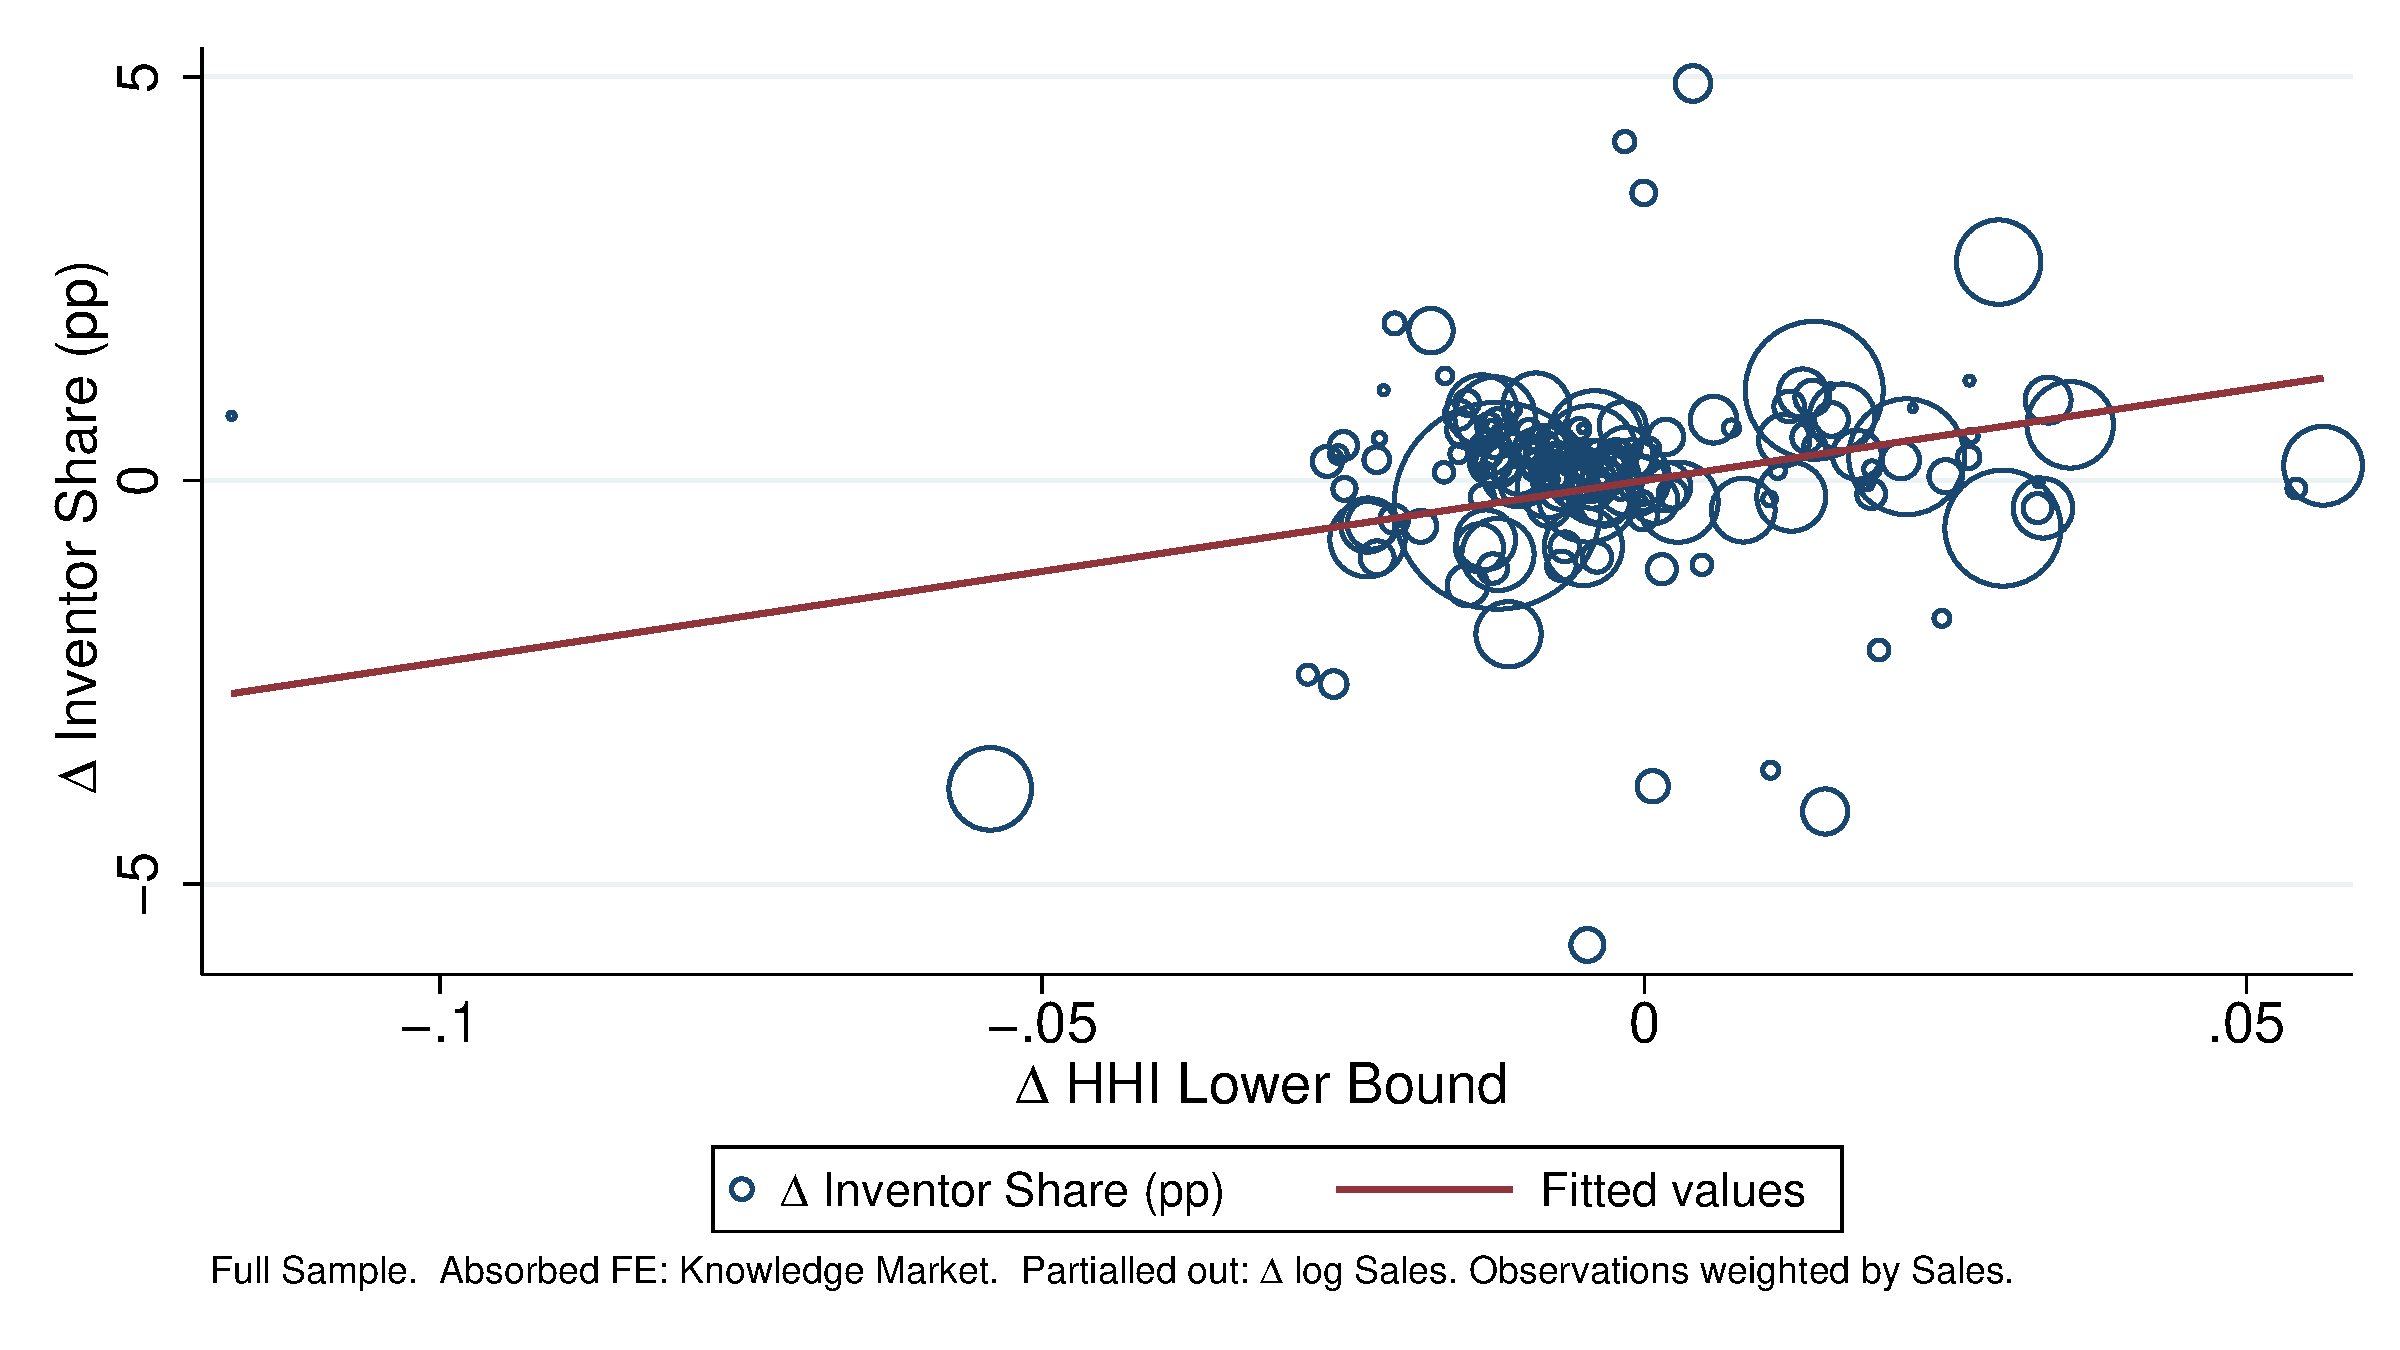
\includegraphics[width=0.9\textwidth]{../graphs/raw_Dk4_hhi_inv_fe10}}

\subfloat[Binned Scatter Plot, Specification in Column (6)]{\centering{}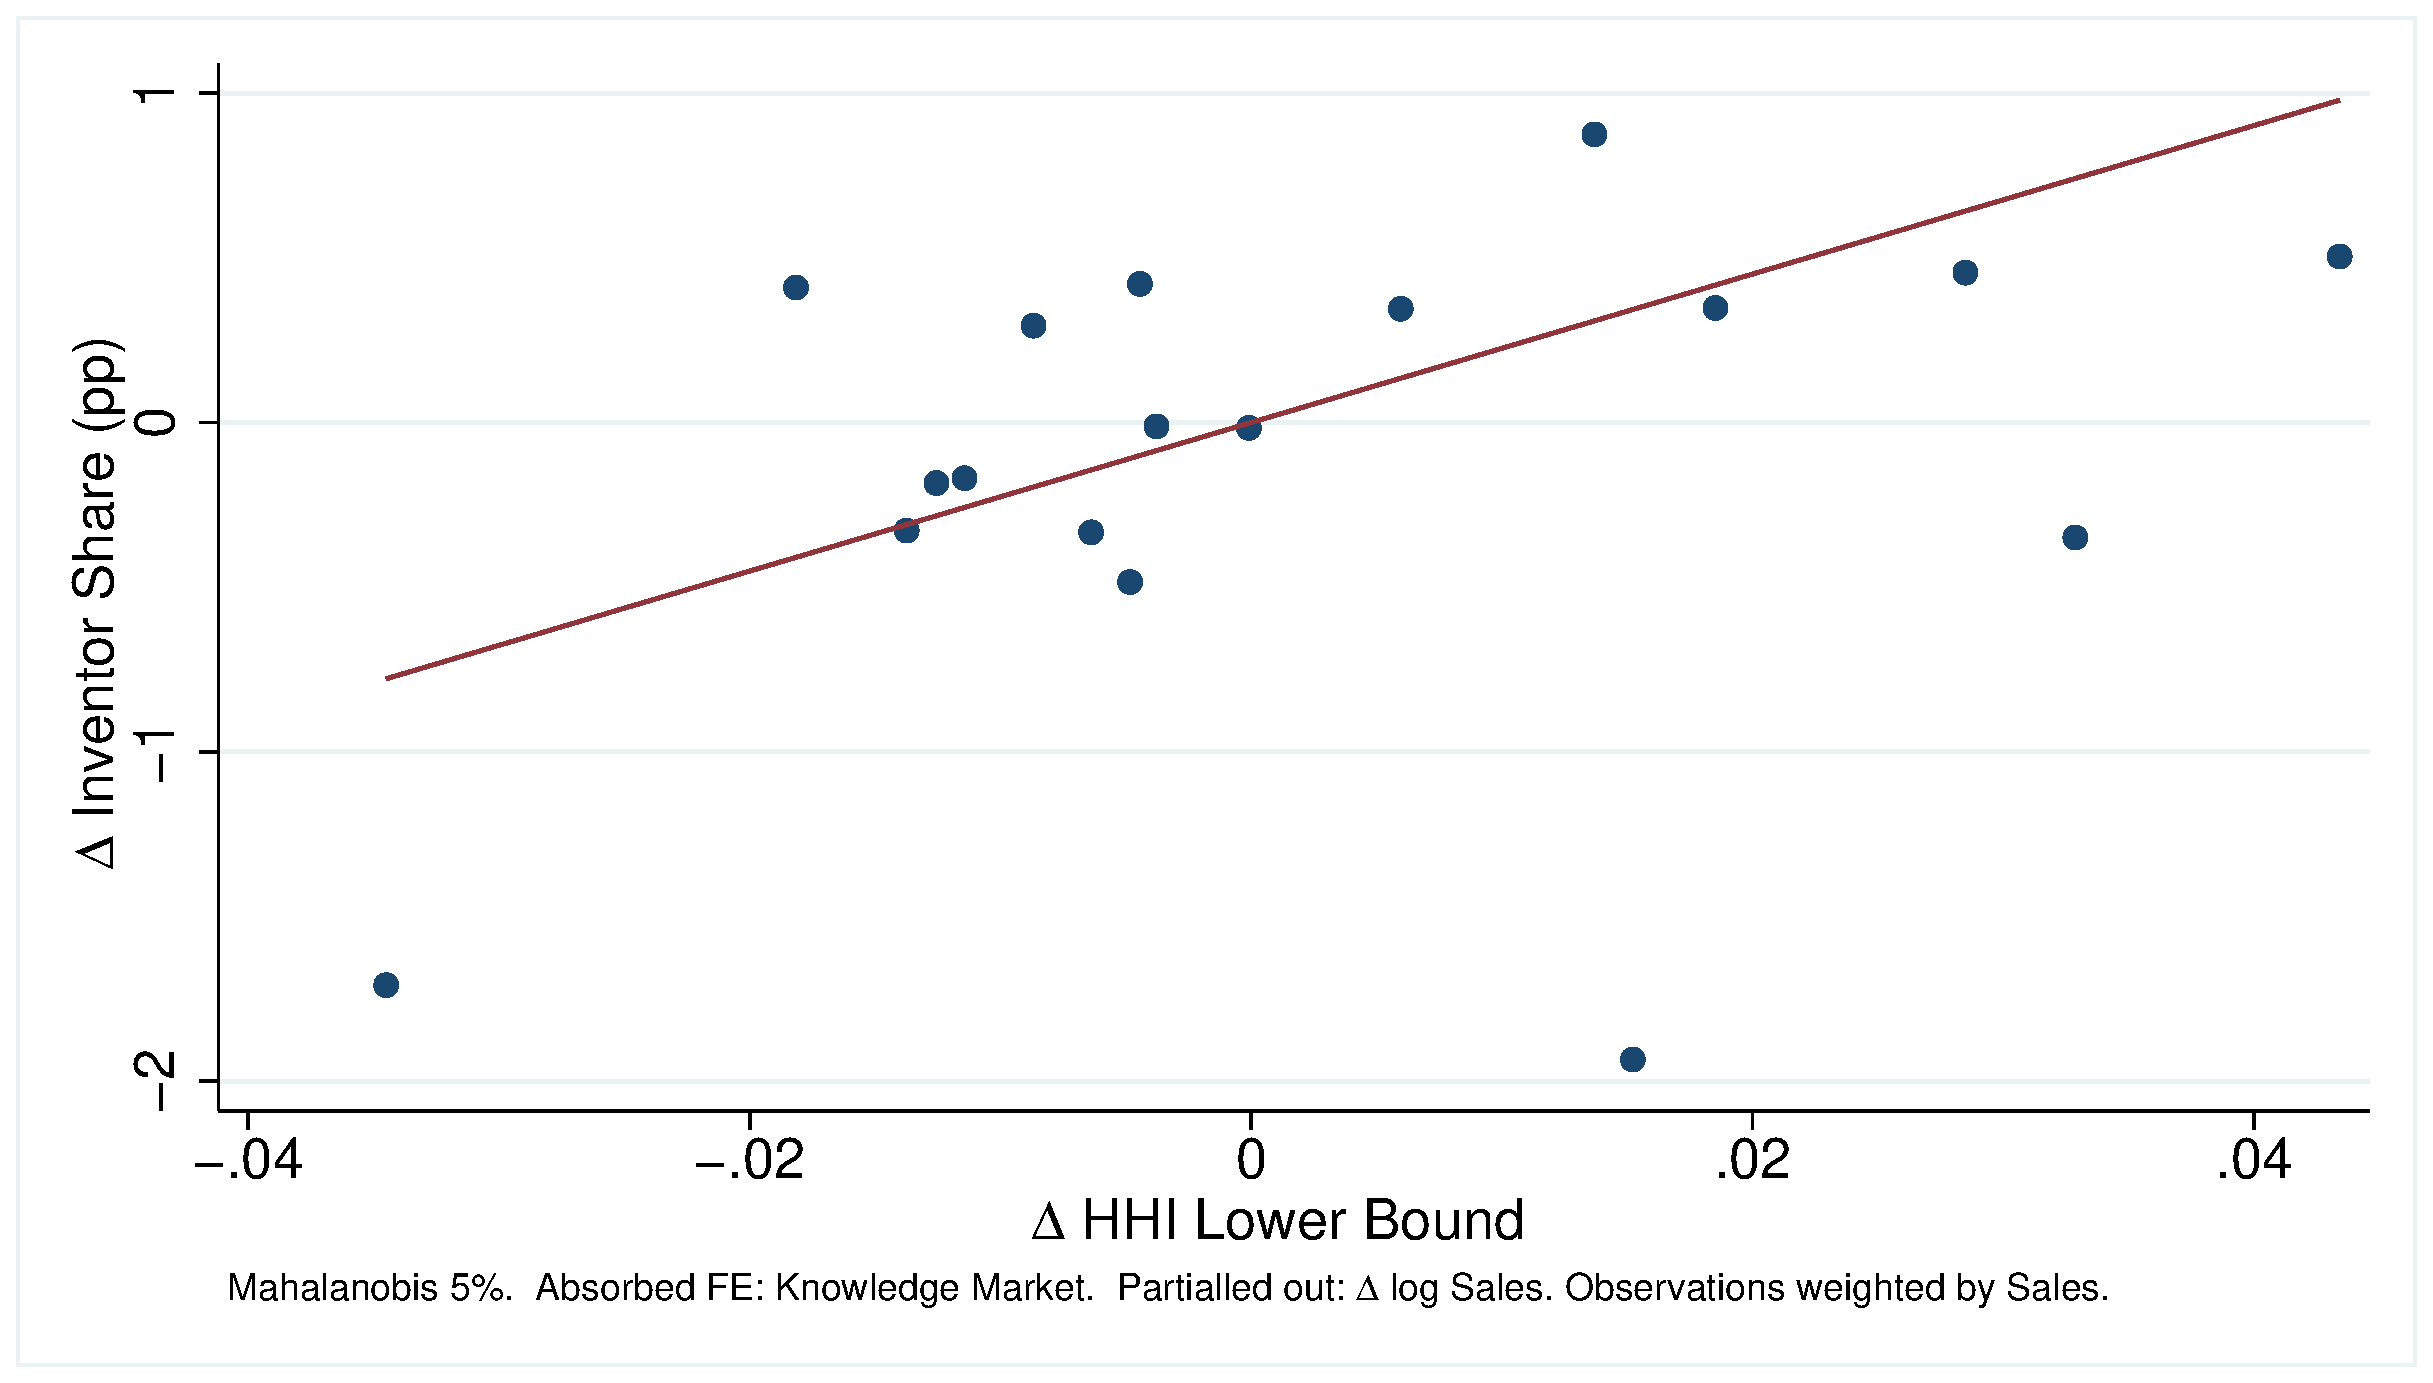
\includegraphics[width=0.9\textwidth]{../graphs/bin_Dk4_hhi_inv_fe12}}\\

\raggedright{}{\small{}Note: This figure presents residualized scatter
plots of the change in the share of effective inventors of sector
$p$ over total inventors in knowledge market $k$, over the change
in the lower bound of the Herfindal-Hirschman Index for product market
$p$, as implied by Census concentration ratios. The upper panel reports
the data for the full sample, where both variables are residualized
by change in log real sales and knowledge market fixed effects. The
size of the markers is proportional to the weight of each observation
in the regression (sector sales in 2012). The regression line uses
the coefficient on the change in HHI lower bound in Column (2) of
Table }\ref{tab: RegShInvHHI}{\small{}. The lower panel presents
a binned scatter plot removing the observations with the highest 5\%
Mahalanobis distance from the sample centroid. Observations are aggregated
using sales weights and the regression line is from Column (6) of
Table }\ref{tab: RegShInvHHI}{\small{}.}{\small\par}
\end{figure}


\paragraph{IV Results}

I now present instrumental variable results that suggest that the
relation between concentration and inventor shares is causal. Indeed,
more concentration could be the result of increasing technological
entry barriers as incumbents hire more R\&D inventors. In this scenario,
the causality would flow from increased inventor shares to higher
concentration. Above, I tried to mitigate this concern using as my
outcome variable the average share of inventors following the Economic
Census years to which the HHI refers. However, reverse causality could
still be present if the autocorrelation of inventor shares is sufficiently
high. As a consequence, I have calculated 2SLS estimates that instrument
the change in the HHI lower bound with changes in product market restrictions,
as measured by the Mercatus dataset RegData 4.0. Theoretically, an
increase in restrictions should raise barriers to entry in affected
product markets, thus leading to higher concentration. As discussed
below, such proves to be the case empirically, validating sector-specific
restrictions as an instrument for concentration. A violation of the
exclusion restriction requires a causal connection between product
market regulations and the share of inventors hired by each sector,
independent of product market concentration. For example, regulations
affecting existing technologies might require more inventors to meet
product market restrictions. However, this effect is unlikely to be
sufficiently large and persistent to be captured by my measure of
inventor shares. Further, the regulations counted in RegData are not
exclusively product restrictions, but also include reporting obligations
and other legal burdens that are not related to technological components.
In addition, while product restrictions might certainly induce a change
in the direction of innovation, there is no a priori reason to believe
that the scale of innovation activity should increase. These considerations
lead me to believe that the exclusion restriction is not likely to
be violated.

The results of the 2SLS estimation are presented in the upper panel
of Table \ref{tab: RegIV}. The specification is the same as in Column
(2) of \ref{tab: RegShInvHHI}, including both knowledge market and
sale change fixed effects. The 2SLS estimates confirm the significance
of concentration changes for the increase in knowledge market inventor
shares. The magnitudes of estimated coefficients are statistically
indistinguishable from the ones reported in the baseline regression.
The first-stage F clearly indicates that instruments are weak. This
is unsurprising since, as detailed above, both the HHI lower bound
and the regulation measures are estimated. In particular, I had to
impute regulations for a large part of the sample using the cosine-similarity
between product market restrictions.\footnote{Using only available sectors requires dropping two thirds of the observations.
See Appendix \ref{app: Data-Construction-Details} for details on
data construction.} However, instruments are not irrelevant. The results in the lower
panel of Table \ref{tab: RegIV} imply that the first-stage t-statistic
for the regression of the change in the HHI lower bound over log-regulations
is 2.07, which corresponds to a p-value of 0.041. The reduced form
regression of inventor share over log restriction change is as highly
significant. Accordingly, the SW underidentification test rejects
the null hypothesis at a 5\% confidence level. Given the weakness
of the instruments, I also report the Anderson-Rubin p-value and the
corresponding confidence intervals in brackets, which confirm that
the coefficient is 5\% significant.

Taken together, the results presented in this section establish a
causal link between the increase in inventor concentration and the
shifts in product market concentration across NAICS 4-digit sectors.

\begin{table}
\caption{IV Regressions of Change in 4-digit Knowledge Market Share over Change
in HHI Lower Bound, 2SLS Long-Difference, 1997-2012\label{tab: RegIV}}

\begin{centering}
\subfloat[2SLS Results]{
\centering{}\scalebox{.9}{{
\def\sym#1{\ifmmode^{#1}\else\(^{#1}\)\fi}
\begin{tabular}{l*{2}{c}}
\hline\hline
                    &$\Delta$ Inventor Share (pp)   &               \\
                    &\multicolumn{1}{c}{(1)}   &\multicolumn{1}{c}{(2)}   \\
\hline
$\Delta \underline{\text{HHI}}$&      32.426+  &      30.096+  \\
                    &    (16.987)   &    (15.819)   \\
                    &$\left[4.850,\  99.013\right]$   &$\left[4.415,\  92.104\right]$   \\
$\Delta \log$ Sales &               &       0.525*  \\
                    &               &     (0.247)   \\
                    &               &$\left[0.525,\  0.525\right]$   \\
\hline
Knowledge Market FE &   \ding{51}   &   \ding{51}   \\
Sample              & Full Sample   &Mahalanobis 5\%   \\
Weight              &       Sales   &       Sales   \\
Observations        &         157   &         150   \\
First-Stage F       &    4.656786   &    4.753009   \\
Anderson-Rubin p-value&    .0298009   &    .0321185   \\
\hline\hline
\end{tabular}
}
}}\\
\subfloat[First Stage and Reduced Form]{
\centering{}\scalebox{1}{{
\def\sym#1{\ifmmode^{#1}\else\(^{#1}\)\fi}
\begin{tabular}{l*{2}{c}}
\hline\hline
                    &Ch. 4d K.M. Eff. Inv. Share (\%)   &Ch. HHI lower bound   \\
                    &\multicolumn{1}{c}{(1)}   &\multicolumn{1}{c}{(2)}   \\
\hline
Ch. Log Restricitions (NAICS 4d)&       0.478*  &       0.016*  \\
                    &     (0.220)   &     (0.007)   \\
Ch. Log Real Sales  &       0.539+  &      -0.000   \\
                    &     (0.274)   &     (0.005)   \\
\hline
4D Knowledge Market FE&   \ding{51}   &   \ding{51}   \\
Sample              & Full Sample   & Full Sample   \\
Weight              &       Sales   &       Sales   \\
Observations        &         153   &         153   \\
\hline\hline
\end{tabular}
}
}}\\
\par\end{centering}
\raggedright{}{\small{}Note: Regressions weighted by sales in 2012;
robust standard errors in parentheses; symbols denote significance
levels $\left(+\ p<0.1,^{*}\ p<0.05,^{**}\ p<.01,^{***}\ p<.001\right)$;
checkmarks indicate the inclusion of fixed effects. This table presents
the results of specifications (\ref{eq: spec}), when the outcome
is the share of effective inventors of sector $p$ over total inventors
in knowledge market $k$, and the independent variable is the change
in the lower bound of the Herfindal-Hirschman Index for product market
$p$, as implied by Economic Census concentration ratios, instrumented
by the change in log-restrictions relevant to the NAICS sector. The
lower panel present first-stage and reduced-form relations. ``Full
Sample'' and ``Mahalanobis 5\%'' refer to the samples described
in the main text.}{\small\par}
\end{table}


\subsubsection{Sectors that Attracted More Researchers Saw Increasing Top Firms'
Inventor Shares and Falling Patent Forward Citations}

While the findings presented so far establish a connection between
inventor and product market concentration, they do not establish that
changes in the distribution of researchers across sectors are inefficient.
It would not be unreasonable, for example, to think that more concentrated
sectors saw increased entry as a result of the higher rents captured
by incumbents. Table \ref{tab: RegStats} shows that the opposite
occurred. Specifically, the share of effective inventors accruing
to top inventor-hiring firms increased in the sectors that attracted
more inventors over the period considered, relative to firms with
fewer inventors in the sector\textemdash a finding consistent across
a variety of measures displayed in Columns (1) to (6). These outcomes
suggest that inventors have increasingly concentrated among large
incumbents, that is, sectors that increased their inventor share also
saw a \emph{within-sector} increase in inventor concentration.

Throughout this section, I present results using changes in inventor
shares to focus directly on the correlation between inventor transitions
and their within-sector distribution. Unless otherwise noted, these
findings are robust to using the change in the HHI rather than the
inventor share, as should be expected from the strong correlation
between these two variables reported in previous tables. For this
section, and other patent-based measures, I present robustness results
using the change in the HHI in Appendix \ref{subsec:Patents-with-HHI}.

My next finding suggests that inventor concentration is driven by
a rise in defensive innovation, that is R\&D aimed at protecting the
incumbents' dominant position and raising barriers to entry. Table
\ref{tab: RegFwdCite} shows that inventors' concentration in specific
sectors went hand in hand with a fall in forward citations for patents,
a standard measure of a patent's contribution to further innovations
\citep{hallNBERPatentCitation2001}. The result in Columns (1) and
(2) report two different measures of forward citations that differ
in how the series are corrected for truncation. As discussed in Section
\ref{subsec:Other data and aggregation}, the measure in Column (2)
uses the procedure delineated by \citet{hallNBERPatentCitation2001},
computing the forward citation lag distribution conditioning on the
technology class of the cited patent. Column (2) also conditions on
the technology class of citing patents. Column (3) presents the estimates
relative to patent generality, a measure of patent impact that increases
with the scope of application. The regressions in this table are unweighted
since they rely only on patent data, but results are robust to using
the HHI as a regressor and weighting by sales. I present results for
the full sample, as well as restricting to the middle range of changes
in inventor shares, which contains more than 90\% of the observations.
In both samples, I find a highly significant negative relation between
changes in inventor shares and the fall in forward citations. The
coefficients imply a high semi-elasticity of self citations to changes
in the inventor shares, whereby a 1 percentage point increase in the
share of inventors leads to a 0.2-0.5\% reduction in forward citations.
After dropping extreme observations, I also find a significant decrease
in the generality of the patents, indicating that concentrating sectors
produce less widely applicable patents. However, the generality finding
is not robust to estimating the regression using the HHI as the independent
variable.

The fall in forward citations is a first indication of the presence
of defensive innovation \citep[see, e.g.,][]{guellecPreemptivePatentingSecuring2012}.
In the next section, I show that these patents also appear to do relatively
little to boost productivity, as measured by growth in output per
worker.

Before moving to the results on productivity, I investigate a competing
explanation for my findings on output growth. As highlighted by \citet{acemogluRadicalIncrementalInnovationForthcoming}
and \citet{akcigitGrowthHeterogeneousInnovations2018} among others,
large incumbents have a strong incentive to focus on improving their
own products at the expense of broadly applicable innovation. This
mechanism would also imply that an increase in incumbents' share of
R\&D resources leads to falling innovation productivity. In order
to assess the importance of this channel, and in keeping with the
analysis in \citet{akcigitGrowthHeterogeneousInnovations2018}, I
use the share of self-citations to measure the extent of internal
innovation conducted by firms. Table \ref{tab: RegSelfCite} displays
the results pertaining to this measure. All columns use as dependent
variable the change in excess log self-citations as defined in Section
\ref{subsec:Other data and aggregation}. Columns (1) and (2) build
excess self-citations correcting for the importance of firms' patents
for the CPC group, which reflects the technological classification
of the patent. Columns (3) and (4) use the more narrowly defined CPC
subgroups for robustness. Coefficients are mostly non-significant
and turn negative when knowledge market fixed effects are included.
Column (3) displays a marginally significant coefficient. However,
this result is not robust to using the HHI as regressor and weighting
regressions by sales as in the baseline specification. The findings
in this table suggest that incremental innovation does not drive my
results.

\begin{sidewaystable}[ph]
\caption{Regressions of Change in Inventor Distribution Measures over Change
in 4-digit Knowledge Market Share, Long-Difference, 1997-2012\label{tab: RegStats}}

\begin{centering}
\scalebox{1}{{
\def\sym#1{\ifmmode^{#1}\else\(^{#1}\)\fi}
\begin{tabular}{l*{2}{c}*{3}{H}}
\hline\hline
                    &Ch. Inv. 90/50 Quantile Ratio   &$\Delta$ Top 10\%/Bottom 50\%   &Ch. Inv. Top-50/Bottom-50 Share Ratio   &$\Delta$ Top 10\%   &$\Delta$ Bottom 50\%   \\
                    &\multicolumn{1}{c}{(1)}   &\multicolumn{1}{c}{(2)}   &\multicolumn{1}{H}{(3)}   &\multicolumn{1}{H}{(4)}   &\multicolumn{1}{H}{(5)}   \\
\hline
$\Delta$ Inventor Share (pp)&       0.211+  &       0.243*  &       0.314+  &       0.018** &      -0.008*  \\
                    &     (0.107)   &     (0.097)   &     (0.184)   &     (0.006)   &     (0.004)   \\
$\Delta \log$ Sales &      -0.100   &       0.328   &       0.147   &       0.026   &       0.005   \\
                    &     (0.122)   &     (0.294)   &     (0.316)   &     (0.020)   &     (0.007)   \\
\hline
Knowledge Market FE &   \ding{51}   &   \ding{51}   &   \ding{51}   &   \ding{51}   &   \ding{51}   \\
Sample              & Full Sample   & Full Sample   & Full Sample   & Full Sample   & Full Sample   \\
Weight              &       Sales   &       Sales   &       Sales   &       Sales   &       Sales   \\
Observations        &         118   &         118   &         118   &         118   &         118   \\
\hline\hline
\end{tabular}
}
}\\
\par\end{centering}
\raggedright{}{\small{}Note: Regressions weighted by sales in 2012;
robust standard errors in parentheses; symbols denote significance
levels $\left(+\ p<0.1,^{*}\ p<0.05,^{**}\ p<.01,^{***}\ p<.001\right)$;
checkmarks indicate the inclusion of fixed effects. Please refer to
notes in Table \ref{tab: RegShInvHHI} for further details. Column
(1) uses the ratio in the 90 percentile of effective inventors to
the median as the outcome variable. Columns (2) and (3) instead present
the share ratio, that is the share of effective inventors accruing
to the top 10 or 50\% relative to the share accruing to the bottom
50\% of the distribution within each NAICS sector.}{\small\par}
\end{sidewaystable}

\begin{table}
\caption{Regressions of Changes in Forward Citation over 4-digit Knowledge
Market Share, Long-Differences, 1997-2012\label{tab: RegFwdCite}}

\begin{centering}
\subfloat[Full sample]{\begin{centering}
\par\end{centering}
\centering{}\scalebox{.9}{{
\def\sym#1{\ifmmode^{#1}\else\(^{#1}\)\fi}
\begin{tabular}{l*{3}{c}}
\hline\hline
                    &Ch. in log citations per patent (CPC2 based)   &Ch. in log citations per patent (Total)   &Ch. in patent generality   \\
                    &\multicolumn{1}{c}{(1)}   &\multicolumn{1}{c}{(2)}   &\multicolumn{1}{c}{(3)}   \\
\hline
Ch. 4d K.M. Eff. Inv. Share (\%)&      -0.197***&      -0.227***&      -0.004   \\
                    &     (0.044)   &     (0.051)   &     (0.004)   \\
Ch. Log Real Sales  &      -0.234*  &      -0.258+  &       0.008   \\
                    &     (0.112)   &     (0.148)   &     (0.013)   \\
\hline
4D Knowledge Market FE&   \ding{51}   &   \ding{51}   &   \ding{51}   \\
Sample              & Full Sample   & Full Sample   & Full Sample   \\
Weight              &               &               &               \\
Observations        &         153   &         153   &         153   \\
\hline\hline
\end{tabular}
}
}}
\par\end{centering}

\begin{centering}
\subfloat[Full sample, restricting to the middle range of the change in inventor
shares ($-2\%$ to $+2\%$)]{\centering{}\scalebox{.9}{ {
\def\sym#1{\ifmmode^{#1}\else\(^{#1}\)\fi}
\begin{tabular}{l*{3}{c}}
\hline\hline
                    &$\Delta \log$ Citations/Patent (CPC)   &$\Delta \log$ Citations/Patent (Total)   &$\Delta$ Patent Generality   \\
                    &\multicolumn{1}{c}{(1)}   &\multicolumn{1}{c}{(2)}   &\multicolumn{1}{c}{(3)}   \\
\hline
$\Delta$ Inventor Share (pp)&      -0.545***&      -0.618***&      -0.025*  \\
                    &     (0.113)   &     (0.137)   &     (0.012)   \\
$\Delta \log$ Sales &      -0.232*  &      -0.255+  &       0.008   \\
                    &     (0.109)   &     (0.146)   &     (0.012)   \\
\hline
Knowledge Market FE &   \ding{51}   &   \ding{51}   &   \ding{51}   \\
Sample              & Full Sample   & Full Sample   & Full Sample   \\
Weight              &               &               &               \\
Observations        &         144   &         144   &         144   \\
\hline\hline
\end{tabular}
}
}}\\
\par\end{centering}
\raggedright{}{\small{}Note: Unweighted regressions; robust standard
errors in parentheses; symbols denote significance levels $\left(+\ p<0.1,^{*}\ p<0.05,^{**}\ p<.01,^{***}\ p<.001\right)$;
checkmarks indicate the inclusion of fixed effects. This table present
the results of specification (\ref{eq: spec}), when the outcome is
the log-change in forward citations and the change in patent generality
in sector $p$ over the change in the share of inventors employed
in sector $p$. Column (1) and (2) presents the results when forward
citations are extrapolated the procedure Hall et al. (2000) to avoid
truncation bias. A specific cite-lag distribution over 35 years is
estimated for each pair of cited and citing CPC2-codes. Column (1)
employs the extrapolation scheme by each pair of CPC2 cited and citing
sector. Column (2) applies the extrapolation scheme to total citations
received by each cited patent. Column (3) presents results on the
patent generality measures. All columns exclude self-citations. Upper
panel: full sample; bottom panel: excluding sectors with absolute
increase in the inventor share above 2\%.}{\small\par}
\end{table}
\begin{table}
\caption{Regressions of Change in Excess Self-Citations over 4-digit Knowledge
Market Share, Long-Differences, 1997-2012\label{tab: RegSelfCite}}

\begin{centering}
\scalebox{.9}{{
\def\sym#1{\ifmmode^{#1}\else\(^{#1}\)\fi}
\begin{tabular}{l*{4}{c}}
\hline\hline
                    &$\Delta$ CPC group self-citations   &               &$\Delta$ CPC subgroup self-citations   &               \\
                    &\multicolumn{1}{c}{(1)}   &\multicolumn{1}{c}{(2)}   &\multicolumn{1}{c}{(3)}   &\multicolumn{1}{c}{(4)}   \\
\hline
$\Delta$ Inventor Share (pp)&       0.920   &      -0.444   &       0.958+  &      -0.228   \\
                    &     (0.711)   &     (1.083)   &     (0.512)   &     (0.801)   \\
$\Delta \log$ Sales &      -1.841   &      -1.954   &      -1.456   &      -1.674   \\
                    &     (1.925)   &     (1.988)   &     (1.326)   &     (1.279)   \\
\hline
Knowledge Market FE &               &   \ding{51}   &               &   \ding{51}   \\
Sample              & Full Sample   & Full Sample   & Full Sample   & Full Sample   \\
Weight              &               &               &               &               \\
Observations        &         157   &         153   &         157   &         153   \\
\hline\hline
\end{tabular}
}
}
\par\end{centering}
\begin{centering}
\par\end{centering}
\raggedright{}{\small{}Note: Unweighted regressions; robust standard
errors in parentheses; symbols denote significance levels $\left(+\ p<0.1,^{*}\ p<0.05,^{**}\ p<.01,^{***}\ p<.001\right)$;
checkmarks indicate the inclusion of fixed effects. This table presents
the results of specifications (\ref{eq: spec}), when the outcome
is the change in excess self-citations in sector $p$ over the change
in the share of inventors employed in sector $p$. }{\small\par}
\end{table}
\FloatBarrier

\subsubsection{Markets with Growing Inventor Shares Experienced a Fall in Inventor
Productivity}

Table \ref{tab: RegProd} presents the results of running (\ref{eq: spec})
when the outcome is the average growth in output per worker per effective
inventor. I use growth in annual output per worker provided by the
Economic Census and average this measure over the five-year window
starting in the Economic Census year, and I analogously build a measure
of average effective inventors over the same period. Inventor productivity
is then defined as average output per worker growth divided by average
number of effective inventors. Both the outcome and the dependent
variable are measured in percentage points. Table \ref{tab: RegProd}
reveals a negative and significant correlation between the increase
in the number of effective inventors and inventor productivity, regardless
of the independent variable employed and the sample restriction adopted.

Starting from the upper panel of Table \ref{tab: RegProd}, the median
change in the share of effective inventors over the period was $.014\text{pp}$,
while the measure of effective inventors has a median of 2018.\footnote{Recall that effective inventors in each year are measured as the sum
of inventor fixed-effects in each year, and therefore do not represent
the simple count of inventors.} The coefficient for concentration in Column (4) implies a fall of
$.15\text{pp}$ ($-.005\times.014\text{pp}\times2018$) in average
annual labor productivity growth. This number decreases to $-.28\text{pp}$
when considering only sectors with positive growth in labor productivity,
which accounted for the bulk of the increase in inventor shares. An
alternative back-of-the-envelope computation, using the change in
product market concentration to predict the change in inventor shares
gives even starker results. Using the coefficient in Column (2) of
Table \ref{tab: RegShInvHHI}(a) and considering a median change in
the HHI of $0.002$ yields an increase in the share of effective inventors
in concentrating sectors of $0.045\text{pp}$. This implies a fall
in average labor productivity implied by misallocation of 0.45pp.
While these numbers might appear large considering the entirety of
the economy, it is worth noting that my sample includes mainly manufacturing
and retail sectors, which experienced a sizable reduction of $2.73pp$
in average annual productivity growth from 1997 to 2012, driven by
a steep decline in output per worker growth in manufacturing. Therefore,
the mechanism I propose would explain around 15 percent of the observed
decrease in output per worker growth in these sectors.

The estimates in the lower panel of Table \ref{tab: RegProd}, which
uses the HHI instead the change in inventor shares as independent
variable, imply even larger growth effects. Using the estimates in
Column (2), a median HHI change of 0.02 and a median number of effective
inventors of 1421 in sectors with growth in inventor shares implies
a $-0.78$pp change in output per worker growth from misallocation,
with a confidence interval ranging from $-0.13$pp to $-1.45$pp.
The midpoint of these estimates would explain $28.6\%$ of the observed
fall in output per worker growth over the sample period ($-2.73\text{pp}$),
with bounds ranging from $4.8\%$ to $53\%$.

This last set of results further supports the hypothesis that defensive
innovation increased in concentrating sectors. To protect their dominant
position, firms engage in such R\&D to thwart innovation by potential
competitors. Similarly citing defensive innovation as a motive, \citet{argentePatentsProductsProduct2020a}
report that incumbent firms tend to register a large number of patents,
but account for a small share of overall innovations.

\begin{table}[h]
\caption{Regressions of Changes in Inventor Productivity over Changes in Inventors'
Share and HHI, Long-Difference, 1997-2012\label{tab: RegProd}}

\begin{centering}
\subfloat[Change in Inventors' Share as Independent Variable]{
\centering{}\scalebox{.95}{{
\def\sym#1{\ifmmode^{#1}\else\(^{#1}\)\fi}
\begin{tabular}{l*{4}{c}}
\hline\hline
                    &$\Delta$ Growth/Inventor (pp)   &               &               &               \\
                    &\multicolumn{1}{c}{(1)}   &\multicolumn{1}{c}{(2)}   &\multicolumn{1}{c}{(3)}   &\multicolumn{1}{c}{(4)}   \\
\hline
$\Delta \underline{HHI}$  &      -0.332** &      -0.292*  &      -0.332** &      -0.290*  \\
                    &     (0.113)   &     (0.123)   &     (0.114)   &     (0.126)   \\
$\Delta \log$ Sales  &               &      -0.052*  &               &      -0.053*  \\
                    &               &     (0.021)   &               &     (0.022)   \\
\hline
Knowledge Market FE&   \ding{51}   &   \ding{51}   &   \ding{51}   &   \ding{51}   \\
Sample              & Full Sample   & Full Sample   &Mahalanobis 5\%   &Mahalanobis 5\%   \\
Weight              &       Sales   &       Sales   &       Sales   &       Sales   \\
Observations        &         101   &         101   &          98   &          94   \\
\hline\hline
\end{tabular}
}
}}\\
\subfloat[Change in HHI as Independent Variable]{
\centering{}\scalebox{.95}{{
\def\sym#1{\ifmmode^{#1}\else\(^{#1}\)\fi}
\begin{tabular}{l*{4}{c}}
\hline\hline
                    &$\Delta$ Growth/Inventor (pp)   &               &               &               \\
                    &\multicolumn{1}{c}{(1)}   &\multicolumn{1}{c}{(2)}   &\multicolumn{1}{c}{(3)}   &\multicolumn{1}{c}{(4)}   \\
\hline
$\Delta \underline{\text{HHI}}$&      -0.332** &      -0.292*  &      -0.332** &      -0.290*  \\
                    &     (0.113)   &     (0.123)   &     (0.114)   &     (0.126)   \\
$\Delta \log$ Sales &               &      -0.052*  &               &      -0.053*  \\
                    &               &     (0.021)   &               &     (0.022)   \\
\hline
Knowledge Market FE &   \ding{51}   &   \ding{51}   &   \ding{51}   &   \ding{51}   \\
Sample              & Full Sample   & Full Sample   &Mahalanobis 5\%   &Mahalanobis 5\%   \\
Weight              &       Sales   &       Sales   &       Sales   &       Sales   \\
Observations        &         101   &         101   &          98   &          94   \\
\hline\hline
\end{tabular}
}
}}\\
\par\end{centering}
\raggedright{}{\small{}Note: Regressions weighted by sales in 2012;
robust standard errors in parentheses; symbols denote significance
levels $\left(+\ p<0.1,^{*}\ p<0.05,^{**}\ p<.01,^{***}\ p<.001\right)$;
checkmarks indicate the inclusion of fixed effects. Please refer to
notes in Table \ref{tab: RegShInvHHI} for further details. Inventor
productivity is measured as the average growth in output per worker
over the five years starting in the Economic Census year over the
total number of effective inventors in each sector. The upper panel
presents estimates when the independent variable is the change in
the share of inventors accruing to a sector, while the bottom panel
uses the change in the lower bound of the HHI index.}{\small\par}
\end{table}
\FloatBarrier
\end{document}



\section{Model\label{sec:Model}}

This section presents a Schumpeterian model based on \citeauthor{abramsPatentValueCitations2013},
featuring growth through creative destruction by entrants, as well
as the possibility for incumbent monopolist of researching a defensive
technology that increases research costs for entrants. I first present
a single-sector model to clarify the mechanism at play within each
sector in the economy and study the properties of a constant-growth
equilibrium analytically. I derive sufficient conditions under which
markup increases lower R\&D productivity, and show that this occur
only if the distribution of inventors shifts in favor of incumbent
firms carrying out defensive innovation.\footnote{In the empirical analysis, I used the HHI as a measure of concentration
and market power. Appendix \ref{app:Using-the-Lerner} shows that
the Lerner Index from NBER-CES, a standard measure of markups, is
strongly correlated with the HHI in my sample, justifying the reduced-form
mapping I adopt in this section.} I also show that in this model, when the supply of inventors is rigid,
inventors' productivity is unaffected by markup changes. Then, I move
to consider a two-sector model, where each sector is identical to
the single-sector model, and the supply of inventors is perfectly
rigid, which shuts down within-sector misallocation occurring independently
of inventors' movements across sectors. I show that increasing markups
in one of the two sectors of the economy lead to a misallocation of
R\&D resources towards defensive innovation in the less competitive
sector. Finally, I study the optimal allocation of R\&D subsidies
needed to achieve maximum growth in a calibration of the two-sector
model that matches moments of the R\&D distribution in 1997, the starting
year for my empirical analysis.

All omitted proofs are reported in Appendix \ref{app: Omitted-Proofs}.

\subsection{Single-sector Model}

\subsubsection{Preferences and production\label{subsec:Preferences-and-production}}

Consider the following continuous time economy with a single final
good. There is a representative household with King-Plosser-Rebelo
preferences over consumption and R\&D labor: 
\begin{equation}
\mathbb{E}_{t}\int_{t}^{\infty}\exp\left(-\rho\left(s-t\right)\right)\left(\ln C_{s}-\frac{\chi\left(L_{s}^{RD}\right)^{1+\frac{1}{\phi}}}{1+\frac{1}{\phi}}\right)\mathrm{d}s,\label{eq:Utility}
\end{equation}
where $\phi$ is the Frisch labor supply. In addition, the representative
household inelastically supplies $L$ units of production labor.\footnote{While this assumption is not necessary for the results to hold, it
simplifies the analysis considerably. In the following section, I
will consider both production and research labor as given by a fixed
endowment in the constant growth equilibrium of the economy. In that
case, the assumption is equivalent to assuming that both labor endowments
grow at a constant rate.} The representative household owns a differentiated portfolio of all
the firms in the economy, with rate of return $r_{t}$, and receives
a wages $w,w^{RD},$ for each unit of production and research labor,
respectively. I assume that the economy is closed and that the final
good is only used for consumption, $C_{t}=Y_{t}$. The above utility
function yields the Euler equation:
\[
\frac{\dot{C_{t}}}{C_{t}}=r_{t}-\rho,
\]
as well as a R\&D labor supply:
\[
L_{t}^{RD}=\left(\frac{w_{t}^{RD}}{\chi C_{t}}\right)^{\phi}.
\]

The consumption good in the economy in each instant is a Cobb-Douglas
aggregate of a measure-one continuum of products:
\begin{equation}
\ln Y_{t}=\int_{0}^{1}\ln y_{t}(i)\mathrm{d}i\label{eq:Y}
\end{equation}
The consumption good in the economy is taken as the numeraire. The
market for each product $y_{t}(i)$ consists of an incumbent and a
fringe of competitors. In what follows, I focus on a single market,
dropping the argument $i$. Each agent $j$ in the sector has the
linear production technology:
\[
y_{j,t}=c_{j,t}l_{j,t},
\]
where $c_{j,t}$ denotes the labor requirement for agent $j$ to produce
a unit of output, and $l_{j,t}$ denotes the production labor employed
by the firm. The incumbent and competitors produce undifferentiated
goods, and differ in their labor requirement. Competitors have labor
requirement, $c_{e,t}=c_{t}$, while the incumbent faces a lower unit
labor requirement $c_{I,t}=\frac{c_{t}}{\phi}$, with $\phi>1$. The
incumbent maximizes profits by choosing a price $p_{t}$ for her product.
Profit maximization gives an optimum limit price $p_{t}=w_{t}c_{t}$,
which leads her to capture the entire market realizing profits:
\[
\Pi_{t}=\left(c_{e,t}-c_{I,t}\right)w_{t}y_{t}=\left(\frac{\phi-1}{\phi}\right)c_{t}w_{t}y_{t}.
\]
Therefore, the incumbent acts as a monopolist, charging a markup $\phi>1$
on its marginal cost. By the Cobb-Douglas assumption on the final
good, the demand facing each product line is:
\[
y_{t}=\frac{Y_{t}}{p_{t}}=\frac{Y_{t}}{w_{t}c_{t}}.
\]
Therefore, equilibrium normalized profits read:
\[
\frac{\Pi_{t}}{Y_{t}}\equiv\pi=\left(\frac{\phi-1}{\phi}\right).
\]


\subsubsection{Innovation}

Both incumbents and entrants can conduct innovation activity that,
if successful, reduces their unit costs to

\[
c_{I,t+\Delta_{t}}=\frac{c_{e,t}}{\left(1+\eta\right)\phi},\quad\eta>1
\]
Here, $\eta$ parametrizes the percentage increase in productivity
for the innovating firm, relative to the technology previously operated
by the incumbent. I assume that there are spillovers from realized
innovations as follows. Whenever either the incumbent or an entrant
realize an innovation, all other firms gain access to a technology
with unit costs
\[
c_{e,t+\Delta_{t}}=\frac{c_{e,t}}{\left(1+\eta\right)}.
\]
These assumptions imply that, if entrants realize an innovation, they
outcompete previous incumbents, and become the new monopolists. Displaced
incumbents join the pool of entrants and from instant $t+\Delta t$
onwards operate the technology $c_{e,t+\Delta_{t}}$. This amounts
to assuming that the incumbent's technology becomes obsolete after
displacement.\footnote{An alternative interpretation of this assumption is that incumbents
are forced to scrap the assets needed to operate the innovative technology
upon destruction, so that the technology is no longer available to
them from the following instant onwards. } Technically, this innovation structure allows to avoid keeping track
of the number of realized innovations. Indeed, in each product market
the relative productivity of incumbents relative to entrants is fixed
at $\phi$, making it possible to formulate the choice of innovation
as a recursive problem.

Incumbents' and entrants' innovation differ in two respects. First,
successful incumbents' R\&D produces a \emph{patent wall }of size
$\omega>1$, which decreases the success probability of entrants'
innovations. Second, successful entrants' R\&D results in an implemented
innovation with certainty, while incumbents adopt new technologies
with probability, $\lambda\in[0,1].$ This parameter can be interpreted
in two ways. The first interpretation is that $\lambda$ captures
the probability that the newly discovered technology is compatible
with the incumbents' current production techniques. The second interpretation
is related to the radical nature of incumbents' innovations. A low
value for $\lambda$ reduces the expected productivity improvement
from an innovation by the incumbent. In other words, the lower $\lambda,$
the more incremental are incumbents' innovations. Under these assumptions,
incumbents \emph{always} obtain a patent wall, but they only implement
their innovations with probability $\lambda$.\footnote{This specification connects to the empirical evidence in \citet{argentePatentsProductsProduct2020a},
who show that large incumbent firms tend to produce a large amount
of patents, but implement a small number of product innovations.}

Following \citet{acemogluIntellectualPropertyRights2012}, I assume
that innovation investments consist in the choice of an arrival rate
of new discoveries, $x_{I}$, and that R\&D costs are increasing and
convex in this arrival rate. In particular, I specify incumbents'
R\&D costs as:
\[
C\left(x_{I};w^{RD}\right)=\alpha_{I}\frac{x_{I}^{\gamma}}{\gamma}w^{RD},\ \gamma>1,
\]
where the term, $\alpha_{I}\frac{x_{I}^{\gamma}}{\gamma}$, indicates
the amount of inventors that the incumbent needs to obtain innovations
with a flow probability, $x_{I},$and $w^{RD}$ is the wage paid to
inventors. For simplicity, I assume that incumbents can only have
one available innovation at a time. That is, incumbents can only erect
\emph{one} patent wall of size $\omega>1$, and cannot invest in further
innovation until this wall is destroyed at a rate, $\delta$, which
captures the rate of patent expiration.

Given these assumptions incumbents' values at any given instant are
just a function of the state of the patent wall in the product market
they operate, $\Omega\in\left\{ 1,\omega\right\} .$ Given the recursive
nature of the problem, I drop time indexes in what follows. Incumbents'
value functions read:
\begin{align}
rV(1)-\dot{V}(1) & =\max_{x_{I}}\left\{ \left(\frac{\phi-1}{\phi}\right)Y-\alpha_{I}\frac{x_{I}^{\gamma}}{\gamma}w^{RD}+x_{I}\left(V(\omega)-V(1)\right)-x_{e,1}V(1)\right\} ,\label{eq:v_1}\\
rV(\omega)-\dot{V}(\omega) & =\left(\frac{\phi-1}{\phi}\right)Y+\delta\left(V(1)-V(\omega)\right)-x_{e,\omega}V(\omega),\label{eq:v_om}
\end{align}
where $x_{e,1}$, $x_{e,\omega}$ denote entrants' innovation intensities,
$r$ is the interest rate in the economy to be determined in equilibrium,
and $\delta$ the rate of patent expiration. The first line displays
the flow value to incumbents that operate in a market not protected
by a patent wall. There, incumbents realize instantaneous profits,
$\left(\frac{\phi-1}{\phi}\right)Y$, and choose their innovation
intensity, $x_{I}$, taking the researchers' wage, $w^{RD}$, as well
as the entrants' innovation intensity $x_{e,1}$, as given. If entrants
are successful at rate $x_{e,1}$, incumbents are destroyed. If incumbents'
innovation is successful at rate, $x_{I}$, they obtain the patent
wall $\omega$, which grants them the protected value, $V(\omega)$.
When a patent wall is in place, incumbents realize the same flow profits
as in the unprotected state, since economy-wide spillovers imply that
incumbents are unable to reap profits from implemented innovations.
However, incumbents face a different entrants' innovation intensity,
$x_{e,\omega}$, which is lower than $x_{e,1}$ due to the patent
wall in place, as I will show below. Finally, incumbents in state
$\omega$ face a flow probability $\delta$ that the patent wall is
exogenously destroyed, in which case they transition back to the unprotected
state. Under these assumptions, the optimal incumbent's R\&D decision
is given by:
\begin{equation}
x_{I}=\bm{1}\left\{ V(\omega)-V(1)>0\right\} \left(\frac{V(\omega)-V(1)}{\alpha_{I}w^{RD}}\right)^{\frac{1}{\gamma-1}}.\label{eq:RD_I}
\end{equation}

Following \citeauthor{abramsPatentValueCitations2013}, I assume that
each market has a mass of atomistic entrants, indexed by $j$, who
face innovation costs that feature congestion externalities:
\[
C\left(x_{e,\Omega,j};w^{RD}\right)=\zeta\Omega x_{e,\Omega,j}x_{e,\Omega}w^{RD}.
\]
In this specification, $\zeta$ parametrizes the inventor requirement
to obtain a unit aggregate entrants' innovation rate when the market
is not protected by patent walls, $\Omega=1$. Individuals costs are
linear in the total entrants' research intensity in the product market,
$x_{e,\Omega}\equiv\int_{\mathcal{J}}x_{e,\Omega,j}\mathrm{d}j.$
In other terms, individual entry costs increase with the aggregate
entry rate. I assume that successful entrants obtain a new unprotected
technology, regardless of the state of the market that they target,
capturing the fact that entrants do not obtain the patents deposited
by the previous incumbents, instead implementing entirely new production
techniques. 

Under the above assumptions, the free entry condition for entrants
targeting a market with patent wall $\Omega$ reads:

\[
\max_{x_{e,\Omega,i}}\left\{ x_{e,\Omega,i}V(1)-\zeta\Omega x_{e,\Omega,i}x_{e,\Omega}w^{RD}\right\} .
\]
This condition pins down the entry rate for each product market with
patent wall $\Omega$ as:
\begin{equation}
x_{e,\Omega}=\frac{V(1)}{\zeta\Omega w^{RD}},\quad\Omega\in\{1,\omega\}.\label{eq:RD_e}
\end{equation}
This expression clarifies the effect of defensive innovation in this
model. The size of the patent wall $\omega$ represents the factor
decrease in the entry rate when a defensive innovation is successful. 

\subsubsection{Equilibrium with Constant Growth}

The laws of motion of product markets across protected and unprotected
states is given by:
\begin{align}
\dot{\mu}_{1} & =-\left(x_{I}+x_{e,1}\right)\mu_{1}+\delta\mu_{\omega}+x_{e,\omega}\mu_{e,\omega}+x_{e,1}\mu_{e,1},\label{eq: dist1-1}\\
\dot{\mu}_{\omega} & =-\left(x_{e,\omega}+\delta\right)\mu_{\omega}+x_{I}\mu_{1},\label{eq: dist2-1}
\end{align}
where $\mu_{e,\omega}$ and $\mu_{e,1}$ denote the mass of entrants
targeting protected and unprotected markets, respectively. Equation
(\ref{eq: dist1-1}) states that the mass of unprotected products
decreases when incumbents successfully develop an innovation at flow
probability, $x_{I},$ or entrants displace existing incumbents at
rate, $x_{e,1}$. Products instead become unprotected if existing
patent walls depreciate, or successful entrants become new monopolists.
Conversely, Equation (\ref{eq: dist1-2}) shows that protected markets
loose mass whenever entrants displace existing protected incumbents
or defensive patents depreciate, and gain mass when incumbents in
unprotected markets develop defensive innovations. 

The mass of entrants in the two types of product markets is determined
in equilibrium following the laws of motion:

\begin{align}
\dot{\mu}_{e,1} & =-\left(x_{e,1}+x_{I}\right)\mu_{e,1}+x_{e,1}\mu_{1}+\delta\mu_{e,\omega},\label{eq: dist3-1}\\
\dot{\mu}_{e,\omega} & =-\left(x_{e,\omega}+\delta\right)\mu_{e,\omega}+x_{e,\omega}\mu_{\omega}+x_{I}\mu_{e,1}.\label{eq: dist4-1}
\end{align}
Here, the first line states that the pool of entrants in unprotected
markets looses mass if entrants successfully develop innovations at
rate, $x_{e,1},$ or incumbents make markets protected at rate, $x_{I}.$
The pool of entrants in markets with $\Omega=1$ instead grows when
incumbents get displaced by successful entrants, and rejoin the ranks
of outsiders, or previously protected markets loose their defensive
walls. Equation (\ref{eq: dist4-1}) is obtained analogously. Given
research intensities, clearing in the labor markets for production
and research labor require:
\begin{align}
L & =\int_{0}^{1}l(i)\mathrm{d}i,\label{eq: Lprod}\\
L^{RD} & =\zeta\left(\omega x_{e,\omega}\mu_{e,\omega}+x_{e,1}\mu_{e,1}\right)+\alpha_{I}\frac{x_{I}^{\gamma}}{\gamma}\mu_{1}.\label{eq: LRD}
\end{align}

A constant growth equilibrium of this economy is defined as follows.
\begin{defn}[Constant Growth Equilibrium]
 A constant growth equilibrium is a sequence of values $\left\{ V_{t}(1),V_{t}(\omega)\right\} ,$
production workers' and inventors' wage sequences $\left\{ w_{t}^{RD},w_{t}\right\} $,
and incumbents' and entrants' R\&D decisions $\left\{ x_{I,t},x_{e,1,t},x_{e,\omega,t}\right\} $
such that, given an endowment of production labor, $L$, $L^{RD}$:
(i) incumbents maximize values (\ref{eq:v_1}) and (\ref{eq:v_om}),
taking entrants R\&D decisions as given, (ii) entrants' R\&D decisions
satisfy (\ref{eq:RD_I}) and (\ref{eq:RD_e}) taking $V_{t}(1)$ as
given, (iii) the distribution of incumbents and entrants across protected
and unprotected markets is constant, $\dot{\mu}_{1}=\dot{\mu}_{\omega}=\dot{\mu}_{e,1}=\dot{\mu}_{e,\omega}=0$
in Equations (\ref{eq: dist1-1})-(\ref{eq: dist4-1}), (iv) values
in each instant are determined by (\ref{eq:v_1}) and (\ref{eq:v_om}),
(v) consumers maximize utility (\ref{eq:Utility}) choosing consumption
and R\&D labor optimally, (vi) labor markets clear according to (\ref{eq: Lprod})
and (\ref{eq: LRD}), (vii) product markets clear, $C_{t}=Y_{t}$,
and (vi) aggregate output (\ref{eq:Y}) grows at the constant rate,
$g\equiv\dot{Y}_{t}/Y_{t}.$
\end{defn}
The following proposition summarizes the properties of the constant
growth equilibrium.
\begin{prop}[Existence and Uniqueness of the Constant Growth Equilibrium]
 \label{prop:CGE}For any endowments of production labor, $L$, there
exists a unique constant growth equilibrium. Denoting optimal incumbents'
and entrants' choices as $x_{I}^{\star},x_{e,\omega}^{\star},x_{e,1}^{\star},$
and the masses of incumbents and entrants across states as $\mu_{1}^{\star},\mu_{\omega}^{\star},\mu_{e,1}^{\star},\mu_{e,\omega}^{\star}$,
the constant growth rate of the economy is given by:
\[
g=\eta\left[x_{e,\omega}^{\star}\mu_{e,\omega}^{\star}+x_{e,1}^{\star}\mu_{e,1}^{\star}+\lambda x_{I}^{\star}\mu_{1}^{\star}\right],
\]
and inventors' productivity is given by:
\[
\frac{g}{L^{RD}}=\eta\frac{x_{e,\omega}^{\star}\mu_{e,\omega}^{\star}+x_{e,1}^{\star}\mu_{e,1}^{\star}+\lambda x_{I}^{\star}\mu_{1}^{\star}}{\zeta\left(\omega x_{e,\omega}^{\star}\mu_{e,\omega}^{\star}+x_{e,1}^{\star}\mu_{e,1}^{\star}\right)+\alpha_{I}\frac{\left(x_{I}^{\star}\right)^{\gamma}}{\gamma}\mu_{1}^{\star}}.
\]
\end{prop}
%
The expression for inventors' productivity can be used to obtain a
first intuition of the mechanism through which higher markups lead
to decreased productivity in this model. First, note that a unit of
total entrants' research intensity in either protected and unprotected
markets produces the same growth. Indeed, by the expression for growth,
it is clear that a unit increase in either $x_{e,\omega}^{\star}\mu_{e,\omega}^{\star}$
or $x_{e,1}^{\star}\mu_{e,1}^{\star}$ gives a growth of $\eta$.
However, the unit labor requirement of research intensity in protected
markets is larger than in unprotected markets as a result of defensive
patents. This is evident from the first term at the denominator, that
shows that a unit of total research in protected markets requires
$\zeta\omega$ inventors, compared with just $\zeta$ in unprotected
markets. These facts immediately imply that any force that pushes
entrants towards protected markets will lower their inventor productivity.
One such force is an increase in incumbents' research intensity that
outstrips entrants', which acts to increase $\mu_{e,\omega},$ the
mass of entrants active in protected markets. As I show formally below,
an increase in the markup raises the value of monopolistic positions,
which pushes up both incumbents' and entrants' research intensities,
$x_{I},x_{e,\omega}.$ This results in an increase in $\mu_{e,\omega}$
only if incumbents' R\&D intensity is more elastic than entrants'. 

The following proposition states the main result in this section,
showing that higher markups unambiguously increase research efforts
by incumbents and entrants, and the share of R\&D labor accruing to
incumbents. The proposition also states the main condition for this
result to lead to a fall in overall inventors' productivity in terms
of sufficient statistics. In particular, the incumbents' R\&D elasticity
to markups must be larger than entrants'. This condition is satisfied
in the data, as the estimates in Table \ref{tab: RegStats}, which
show that incumbents increase their share of inventors following increases
in markups. 
\begin{prop}[Effects of Markup Increases on Innovation]
\label{prop: partialEq}Suppose that defensive research is effective,
$\omega>1$. The constant growth equilibrium features positive incumbents'
research, $x_{I}^{\star}>0$, and markup increases raise both incumbents'
and entrants' research effort:
\[
\frac{\partial x_{I}^{\star}}{\partial\phi}>0,\ \frac{\partial x_{e,\omega}^{\star}}{\partial\phi}>0\ \frac{\partial x_{e,1}^{\star}}{\partial\phi}>0,
\]
and the share of R\&D labor employed by incumbents increases with
markup:
\[
\frac{\partial\frac{L_{I}}{L^{RD}}}{\partial\phi}=\frac{\partial\left(\nicefrac{\alpha_{I}\frac{x_{I}^{\gamma}}{\gamma}\mu_{1}}{L^{RD}}\right)}{\partial\phi}>0.
\]
Moreover, if $\lambda=0,$ inventor supply is not fully inelastic,
and the model parameters are such that equilibrium incumbents' research
effort is more elastic than entrants', 
\[
\frac{\partial x_{I}^{\star}}{\partial\phi}\frac{\phi}{x_{I}^{\star}}>\frac{\partial x_{e,\omega}^{\star}}{\partial\phi}\frac{\phi}{x_{e,\omega}^{\star}},
\]
it further holds:
\[
\frac{\partial\left(\nicefrac{g}{L^{RD}}\right)}{\partial\phi}<0.
\]
That is, an increase in the markup, $\phi$, lowers equilibrium inventors'
productivity. 
\end{prop}
The intuition behind this proposition is that increases in the markup
raise the value of monopolistic positions, thus raising both entrants'
and incumbents' research effort. In addition, this leads to an overall
increase in inventors employed by incumbents. Importantly, this holds
only if defensive R\&D is effective, showing the importance of this
channel to reproduce the empirical findings in Table \ref{tab: RegStats}.
However, this finding is not sufficient to generate a fall in inventors'
productivity. This is because the overall change in inventors' productivity
can be decomposed as:
\begin{align*}
\mathrm{d}\left(\frac{g}{L^{RD}}\right) & =\mathrm{d}\left(\frac{L_{e}}{L^{RD}}P_{e}\right)+\mathrm{d}\left(\frac{L_{I}}{L^{RD}}P_{I}\right),
\end{align*}
where $P_{e}$, $P_{I}$ denote entrants' and incumbents' productivity,
respectively. As long as incumbents' productivity is lower than entrants,
a reallocation of inventors towards dominant firm leads to a decrease
in inventors productivity. However, this effect can in principle be
offset by an increase in entrants' productivity. The sufficient conditions
in Proposition \ref{prop: partialEq} ensure that this is not the
case.\footnote{Corollary \ref{cor: parameters} in the Appendix provides parametric
sufficient conditions for the case with quadratic costs, $\gamma=2$,
which is analytically tractable.} In particular, if incumbents' research effort is more elastic than
entrants', an increase in markups reduces the overall share of unprotected
markets, making entry overall more difficult, and reducing entrants'
productivity as well. This reasoning also clarifies why the condition
is sufficient. Indeed, a fall in inventors' productivity occurs as
long as the increase in creative-destruction growth by entrants is
not high enough relative to the increase in defensive innovation by
entrants. As noted above, this condition is satisfied in the data,
and always appear to be in numerical simulations, regardless of specific
assumptions on parameter values. In particular, the assumption $\lambda=0$
is not necessary to generate the result, but I make to obtain clear
analytical results in the proof to this Proposition. 

It is important to stress that the decline in productivity requires
a strictly positive elasticity of inventors' supply. As I show in
Lemma \ref{lem:Labor Demand} in the Appendix, \emph{aggregate} inventor
labor demand is increasing in markups. As a result, when inventors'
supply is fully rigid, wage effects need to fully offset the increase
in labor demand, and by the uniqueness of the CGE, it the allocation
of inventors across incumbents and entrants is fixed. Indeed, aggregate
labor demand is uniquely pinned down by research intensities through
the stationary distribution. 

Figure \ref{fig:OneSecCS} provides a graphical illustration of the
comparative statics for an increase in markup in a calibration of
the one-sector model, which follows the strategy described in detail
in the following Section.\footnote{The parameters of the calibration are chosen to match moments of the
R\&D expenditure distribution as in Section \ref{subsec:Two-sectors},
and the complete set of parameters is reported in Appendix. } An increase in the markup raises profits, thereby increasing the
value of dominant positions, and propelling both incumbents' and entrants'
research. Importantly, the incumbents' inventor demand is more elastic
to increased profits, which raises the overall proportion of researchers
employed in defensive projects. Although overall growth increases
as a result of higher aggregate R\&D, the productivity of inventors
fall, as they get increasingly allocated to incumbents. Two observations
are in order. First, with a fixed supply of inventors, equilibrium
allocations do not change with increased profits, leaving R\&D productivity
unaffected. Second, in the absence of defensive innovation, the increase
in profits would just result in increased entry and growth, leaving
productivity constant.\footnote{In the absence of defensive innovation, the whole mass of firms operates
in unprotected markets and there is no incumbent research. From the
expression for growth in Proposition \ref{prop: partialEq} inventor
productivity is constant at $\nicefrac{\eta}{\zeta}.$}

\begin{figure}[th]
\begin{centering}
\caption{Comparative Statics for Changes in the Markup in the Single-Sector
Model \label{fig:OneSecCS}}
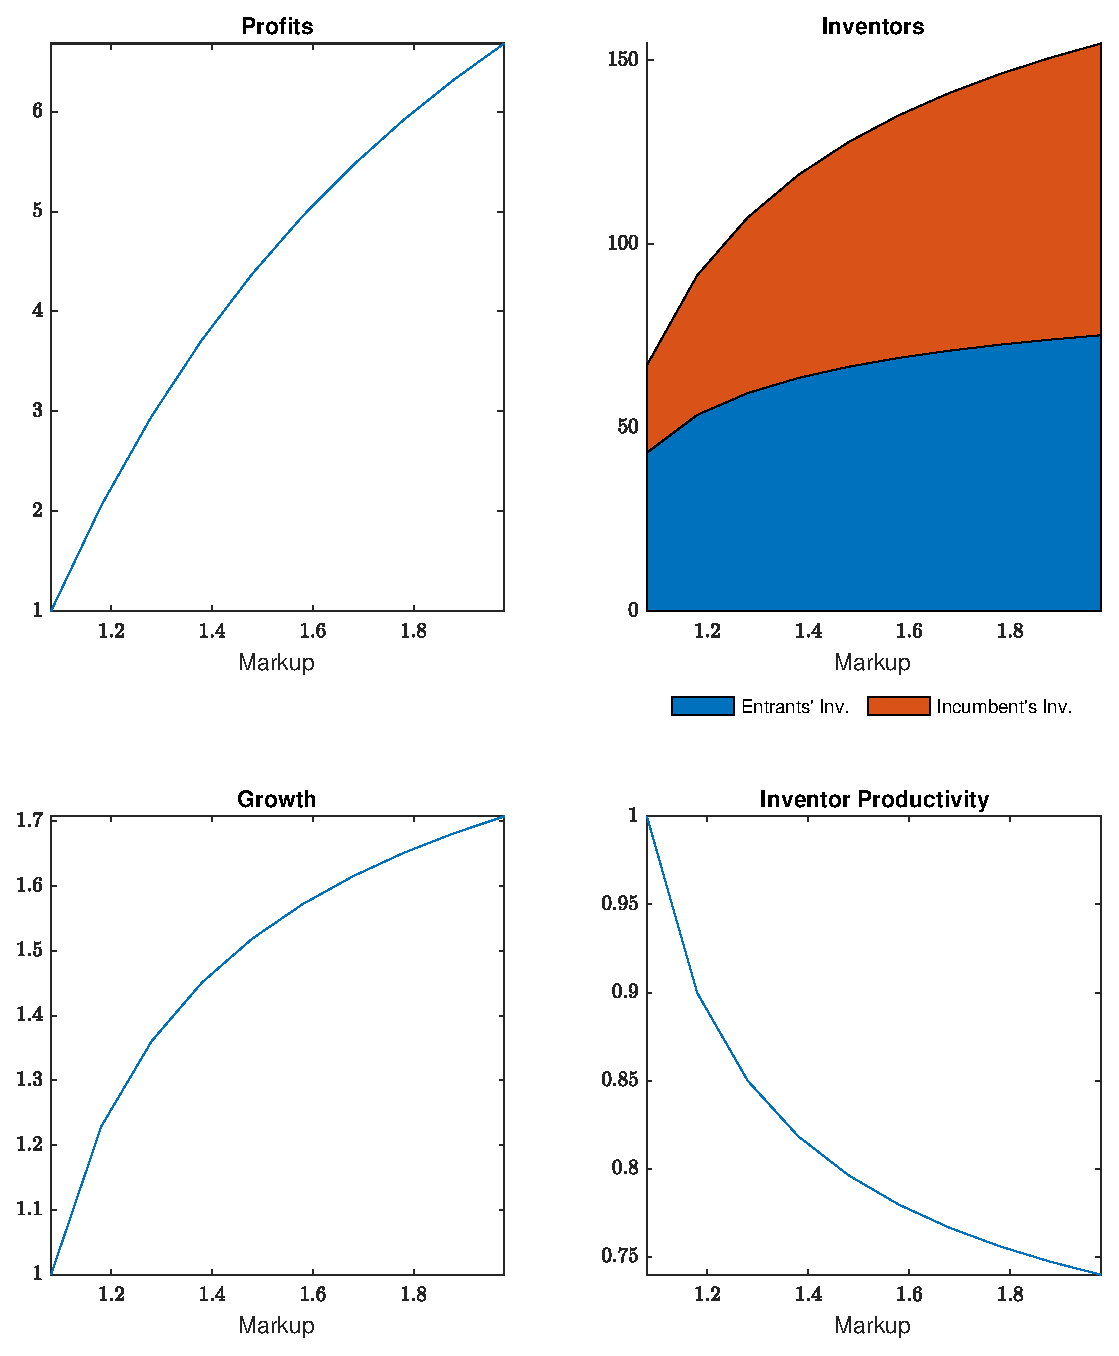
\includegraphics[width=1\textwidth]{graphs/Single_sector}
\par\end{centering}
\raggedright{}{\small{}Note: This figure reports the comparative statics
for normalized profits, inventors, growth and inventor productivity
in the single-sector model. All variables are expressed in units relative
to the equilibrium with $\phi=1.08.$ The calibration follows the
same strategy as in Section \ref{subsec:Calibration}, assuming that
the economy is only composed by a single sector. I set the elasticity
of inventors' supply at $\varphi=1$. }{\small\par}
\end{figure}
\FloatBarrier

\subsection{Calibration and Policy\label{subsec:Two-sectors}}

In this section, I calibrate a two-sector extension of the model presented
in the previous Section, with two main objectives. First, I want to
analyze misallocation \emph{across }sectors, and show that, under
a realistic calibration, this extension can qualitatively reproduce
the main findings of the empirical analysis. I focus on the benchmark
with\emph{ fixed} inventor supply where, by the results in the previous
section, markups have no effect on inventors' productivity within
sectors. This choice excludes that my findings are driven by within-sector
misallocation alone. Second, I wish to study the distribution of R\&D
subsidies across firms that maximizes aggregate growth. The policy
analysis reveals that a planner interested in maximizing growth chooses
to subsidize entry in less competitive sectors, rather than reallocating
inventors back to more competitive sectors. This result arises for
two reasons. First, while misallocation arises only as a result of
flows across sectors, it acts through misallocation within the sector
that becomes more concentrated, where incumbents' defensive research
increases more than entrants' productive R\&D. Second, the outflow
of inventors reduces defensive innovation more competitive sectors.
As a result, reallocating inventors back to competitive sectors would
then come at the cost of inventor productivity in these sectors, while
tackling the misallocation within concentrated sectors only indirectly.

\subsubsection{Model description}

The consumption good in the economy is given by the Cobb Douglas aggregate:
\[
\ln Y_{t}=\beta_{1}\ln Y_{1,t}+\beta_{2}\ln Y_{2,t},\quad\beta_{1}+\beta_{2}=1
\]
where $Y_{1,t}$, $Y_{2,t}$ are produced as in Section \ref{subsec:Preferences-and-production},
and the markup parameter, $\phi$, is allowed to vary across the two
sectors.

The household side of the economy is unchanged relative to the one-sector
model. In this section, however, the supply of inventors is assumed
to be fully rigid and given by $L^{RD}=100.$ This assumption is motivated
by two considerations. First, a fixed inventor supply captures an
aggregate scarcity of inventors, allowing me to focus exclusively
on their allocation across sectors. Second, as discussed above, in
this benchmark markup changes have no effect on misallocation if inventors
are not allowed to move across sectors. Therefore, the results below
isolate the effect of inventors' transitions across sectors on misallocation.

Given the presence of two markets, labor market clearing for production
workers and inventors is now given by:
\begin{align}
L & =\sum_{i=1}^{2}\int_{0}^{1}l_{i,j,t}\left(w^{RD}\right)\mathrm{d}j,\label{eq: Lprod-1}\\
L^{RD} & =\sum_{i=1}^{2}L_{i,t}^{RD}\left(w^{RD}\right),\label{eq: LRD-1}
\end{align}
where the subscript $i$ denotes sectors and $j$ the product markets
in each sector. I define a constant growth equilibrium as in the previous
section. Given the Cobb-Douglas assumption on the final good, growth
is now given by:
\[
\Delta\ln Y_{t}=\sum_{i=1}\beta_{i}g_{i},
\]
where $g_{i}$ denotes the sector-specific output growth obtained
as in Proposition \ref{prop: partialEq}. Appendix \ref{app: twoSec}
reports the derivations for the two-sector model and a complete description
of the equations characterizing the equilibrium.

\subsubsection{Calibration\label{subsec:Calibration}}

I calibrate my model in order to match features of the R\&D distribution
and concentration around 1997, the starting year for my analysis.
The aim of my calibration is to provide a qualitative description
of the features of the model under realistic parameter choices. For
this reason, I do not attempt to match the fall in growth implied
by the model within or across sectors. As I will show below, my calibration
implies a fall in inventors' productivity of about 2\% over the period
1997-2012, about half of the lower bound implied by my empirical estimates.
The calibration is therefore very conservative relative to my empirical
estimates, which provides a useful benchmark to establish a lower
bound of the effects of switching to an optimal R\&D subsidy policy
in the following section. 

Table \ref{tab: intPar} displays my choices for parameters calibrated
externally. I set the discount rate to $4\%$, which, together with
a 3\% growth for my sample in 1997, implies a value for the real interest
rate of 7\%, in line with the long-run average before 1997. I obtain
a value for $\beta$, the share of value added of each sector, from
estimates of the Lerner Index in manufacturing that I obtain from
the NBER-CES as described in Appendix \ref{app:Using-the-Lerner}.
According to these estimates, about half of the sectors (weighted
by sales) for which I have these data saw an increase in the Lerner
Index over the period. This suggests $\beta_{1}=\beta_{2}=0.5.$ Since
I only have the Lerner Index for about half of the sectors, I rely
on the extensive literature estimating markups to set a value of $\phi=1.08$.
In particular, I follow \citet{akcigitWhatHappenedBusiness2019a},
who calibrate the same parameter using the midpoint of estimates provided
in \citet{deloeckerRiseMarketPower2020} and \citet{eggertssonKaldorPikettyFacts2018}.
As standard in the literature \citep[see e.g., ][]{acemogluIntellectualPropertyRights2012},
I set the curvature of the incumbents' cost function relying on the
estimates by \citealp{kortumEquilibriumPatentRatio1993}. I choose
the lower bound of these estimates in order to minimize the asymmetry
of innovation costs between incumbents and entrants, as more convex
incumbents' costs mechanically make incumbents' research, even when
productive, less effective than entrants. The rate of patent expiration
comes directly from the legislative framework in the US, as established
by the Uruguay Round Agreements Act of 1994. Since $\lambda$ measures
how radical are incumbents' innovations relative to entrants', I set
$\lambda=0.785$, the complement of the internal patent share of 21.5\%
estimated by \citet{akcigitGrowthHeterogeneousInnovations2018}. Turning
to the value of blocking patents, parametrized by $\omega$ in my
model, I rely on estimates by \citet{czarnitzkiHowValuableAre2020}
and \citet{grimpePreemptingTechnologyCompetition2008}, who employ
merger data to obtain the effect of pre-emptive patents on the value
of acquired firms. Both their estimates imply an elasticity of firm's
values to the share of patents with pre-emptive value of more than
one. This implies that a firm with a patent portfolio composed exclusively
of defensive patents is valued on average twice as much as one with
only patents that have no pre-emptive value. This suggest a value
of $\omega=2$. As shown in the proof of Proposition \ref{prop:CGE},
my model gives an elasticity of firms' value of at most $\omega-1$,
therefore $\omega=2$ effectively caps this elasticity to $1$. I
also include R\&D subsidies, modeled as a percent subsidy on inventors'
wages,$s$, and corporate taxes applied to firms instantaneous profits,
$\tau$. I set these two parameters following the values reported
by \citet{akcigitOptimalTaxationPolicies2016}.

Table \ref{tab: intPar} describes my choices for the remaining parameters,
that govern the scale of R\&D and the growth rate in the economy.
Specifically, I set the incumbents' and entrants' R\&D cost scale,
$\alpha_{I}$ and $\zeta$, in order to match the share of inventors
employed by incumbent firms in 1997 and the R\&D business spending
as a percent of GDP, as reported by the National Science Foundation.
Intuitively, the two cost parameters jointly determine the overall
R\&D spending in the economy, while their relative value determines
the distribution of R\&D spending in equilibrium. Given the estimates
for $\alpha_{I}$ and $\zeta$, I set $\eta$ to match the growth
in output per worker for the sectors considered in my analysis in
1997, $3.03\%$. All targets are matched almost exactly.\footnote{The average percentage point deviation of moments in the model from
their empirical targets is less than $10^{-6}.$} 

\begin{sidewaystable}
\caption{Parameter Values and Sources}
\subfloat[Parameters Calibrated Externally]{\label{tab: extPar}
\centering{}%
\begin{tabular}{llll}
\toprule 
Parameter Name & Symbol & Value & Source/Target\tabularnewline
\midrule
\midrule 
Discount rate & $\rho$ & .04 & Annual real interest rate $\approx7\%$ before 1997\tabularnewline
Value Added Share & $\beta$ & .5 & Share of sectors with $\uparrow$ Lerner Index\tabularnewline
Average Sectors' Markup & $\phi$ & 1.08 & \citealp{deloeckerRiseMarketPower2020} and \citealp{eggertssonKaldorPikettyFacts2018}\tabularnewline
Innovation Cost Curvature & $\gamma$ & $1/.6$ & Lower bound of estimates in \citealp{kortumEquilibriumPatentRatio1993}\tabularnewline
Intensity of Patent Expiration & $\delta$ & .05 & Uruguay Round Agreements Act (1994)\tabularnewline
Share of Implemented Innovations & $\lambda$ & .785 & Internal patent share of 21.5\% \citep{akcigitGrowthHeterogeneousInnovations2018}\tabularnewline
Value of Blocking Patents & $\omega$ & 2 & \citealp{czarnitzkiHowValuableAre2020,grimpePreemptingTechnologyCompetition2008}\tabularnewline
R\&D subsidy  & $s_{I}=s_{e}$ & 19\% & \citealp{akcigitOptimalTaxationPolicies2016}\tabularnewline
Corporate tax rate  & $\tau$ & 23\% & \citealp{akcigitOptimalTaxationPolicies2016}\tabularnewline
\bottomrule
\end{tabular}}\\

\centering{}\subfloat[Parameters Calibrated Internally]{\label{tab: intPar}
\centering{}%
\begin{tabular}{lccc}
\toprule 
Parameter Name & Symbol & Value & Target\tabularnewline
\midrule
\midrule 
Incumbent Costs & $\alpha_{I}$ & 21.97 & Top 10\% Firms' Inventor Share, 1997: 30.3\%\tabularnewline
Entrants' Costs & $\zeta$ & 4.75 & Business R\&D Share over GDP, 1997: 1.81\%\tabularnewline
Innovation Step & $\eta$ & 0.0047 & Output per Worker Growth, 1997: 3.03\%\tabularnewline
\bottomrule
\end{tabular}}
\end{sidewaystable}


\subsubsection{Comparative Statics in General Equilibrium}

Figure \ref{fig:TwoSecAgg} displays the comparative statics for an
increase in markup in sector 2, while leaving the other sector's markup
unchanged. The graphs compares the aggregates of interest across different
constant growth equilibria, and each figure reports the markup of
sector 2 relative to sector 1 on the x-axis. 

An increase in the relative markup of sector 2 leads to a pronounced
reallocation of inventors away from sector 1. In sector 2, incoming
inventors are allocated disproportionately to incumbents, who expand
their share of researchers relative to entrants. This leads to a decrease
in overall inventor productivity of about Computing the Lerner Index
on NBER-CES data as described in Appendix \ref{app:Using-the-Lerner}
reveals that the markup gap between more concentrated and less concentrated
sectors has increased by about 20\% over the period of interest. This
implies a fall in inventors' productivity of about 2\% compared to
the benchmark where the two sectors have the same competitive structure.
Since the supply of inventors is fixed at $L^{RD}=100$, this results
in a $2.5\%$ fall in GDP growth, about 0.075pp. This estimate is
close to the lower bound of 0.13pp implied by my estimates in Table
\ref{tab: RegProd}. As discussed above, assuming an inelastic labor
supply mutes the response of inventors' productivity to increases
in the markup, so it is reasonable to expect the model in this section
to understate the productivity effects of increased concentration.
However, this benchmark is desirable since it shuts down productivity
effects unrelated to reallocation.

Figure \ref{fig:TwoSecSectors} shows the changes occurring in each
sector that correspond to the aggregates reproduced in Figure \ref{fig:TwoSecAgg}.
In this figure all variables are normalized by their value in the
initial equilibrium with $\phi_{1}=\phi_{2}=1.08.$ Starting from
the upper-left panel, increasing markups raise profits in sector 2
relative to sector 1. This shift translates into an increase in inventors
in sector 2 relative to sector 1. The upper-right panel show that
incumbents' inventor demand is more elastic in response to increases
in the markup, which raises top firms' share in sector 2. The increase
in the equilibrium inventors' wage leads to a reallocation within
sector 1 as well, where entrants gain inventors relative to incumbents.
As a result of these shifts, growth increases in sector 2, and falls
in sector 1, while inventors' productivity follows the opposite pattern.

The reallocation of inventors within sector 1 is a feature of the
model that will be important to interpret the policy results in the
following section. The specular behavior of sectors 1 and 2 reveals
the crucial role of the overall R\&D activity in shaping inventor
productivity. In particular, the incentives to conduct defensive innovation
increase when there is a larger number of inventors employed in the
sector. Therefore, while the movements of inventors from sector 1
to sector 2 are overall detrimental to growth, they are not for R\&D
productivity in sector 1. Since incumbents there face a lower risk
of being displaced by entrants, they reduce their efforts in defensive
innovation, which increases R\&D productivity in sector 1. However,
overall growth is lower since less R\&D resources are available to
this sector in equilibrium. Overall, the results in this section suggest
that inventor reallocation away from competitive sectors has both
costs, resulting from a reduction in sectoral growth, and benefits,
coming from a more efficient distribution of resources within this
sector. 

This comparative static exercise also clarifies that defensive innovation
is crucial to generate misallocation across sectors. In the absence
of defensive innovation, just reallocate across sectors, leaving productivity
unaffected, and as a result overall growth is also unchanged, since
the Cobb-Douglas assumption with $\beta=0.5$ gives aggregate growth
as the simple average of growth in the two sectors.

\begin{figure}[th]
\begin{centering}
\caption{Comparative Statics in Sector 2's Markup Relative to Sector 1 in the
Two-Sector Model, Economy Aggregates \label{fig:TwoSecAgg}}
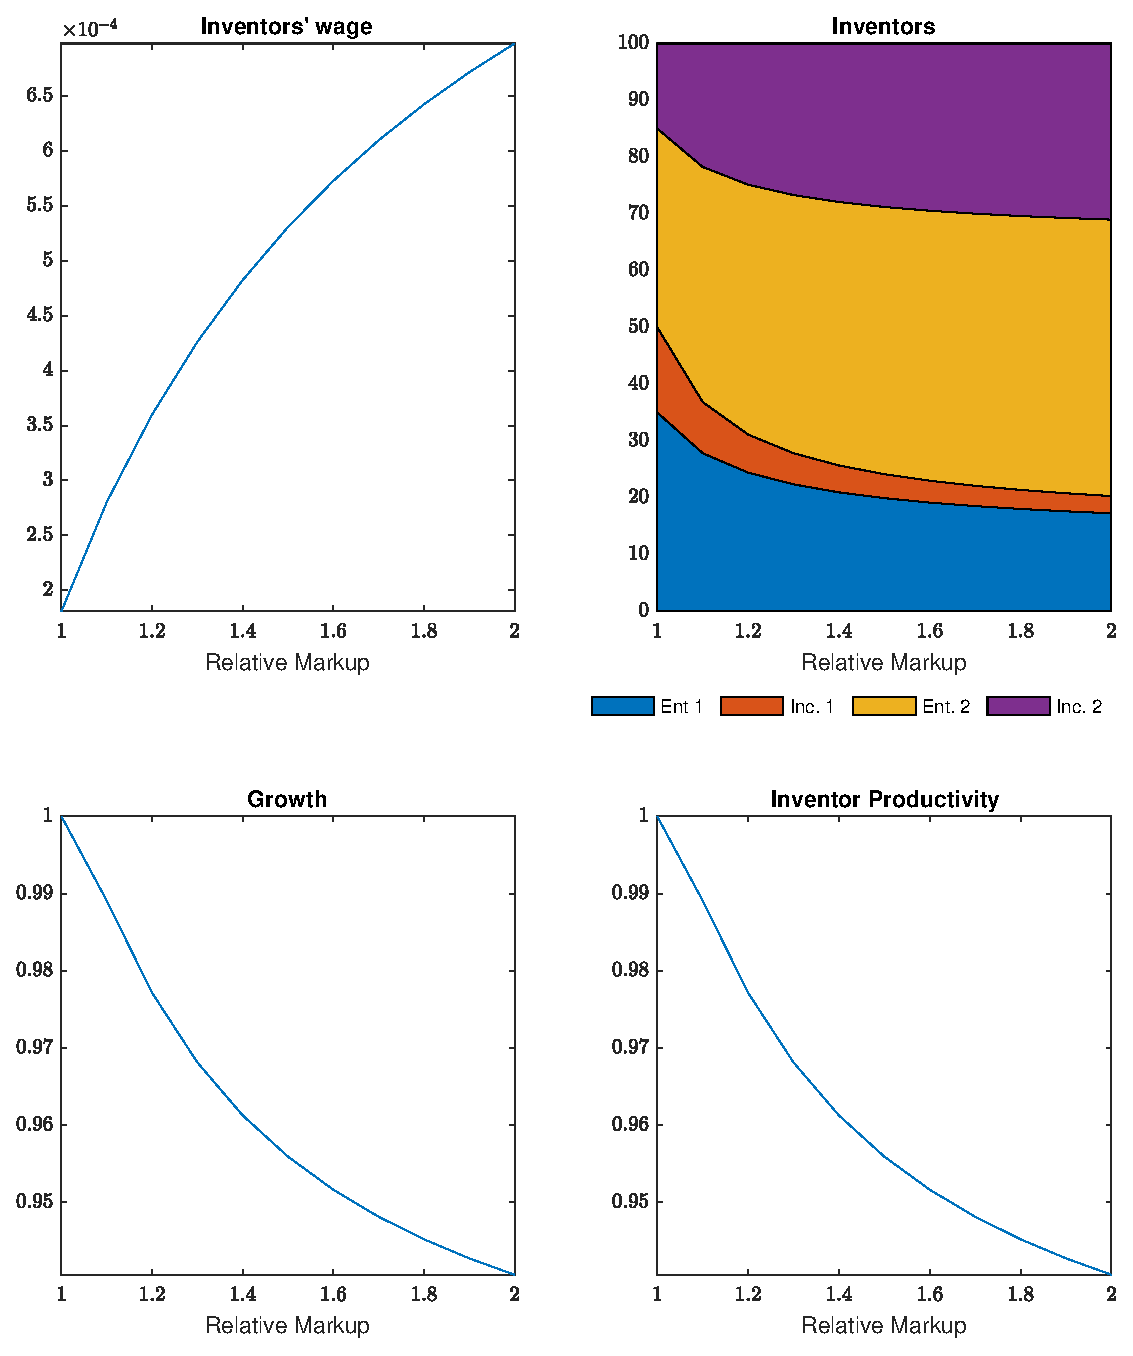
\includegraphics[width=1\columnwidth]{graphs/GE_aggregates}
\par\end{centering}
\raggedright{}{\small{}Note: This figure reports the comparative statics
for normalized profits, inventors, growth and inventor productivity
in the two-sector model. In all figures, the x-axis reports the markup
of sector 2 relative to sector 1. The parameters used to produce this
Figure are reported in Tables \ref{tab: extPar} and \ref{tab: intPar}.}{\small\par}
\end{figure}
\begin{figure}[th]
\begin{centering}
\caption{Comparative Statics in Sector 2's Markup Relative to Sector 1 in the
Two-Sector Model, Sector-level Aggregates \label{fig:TwoSecSectors}}
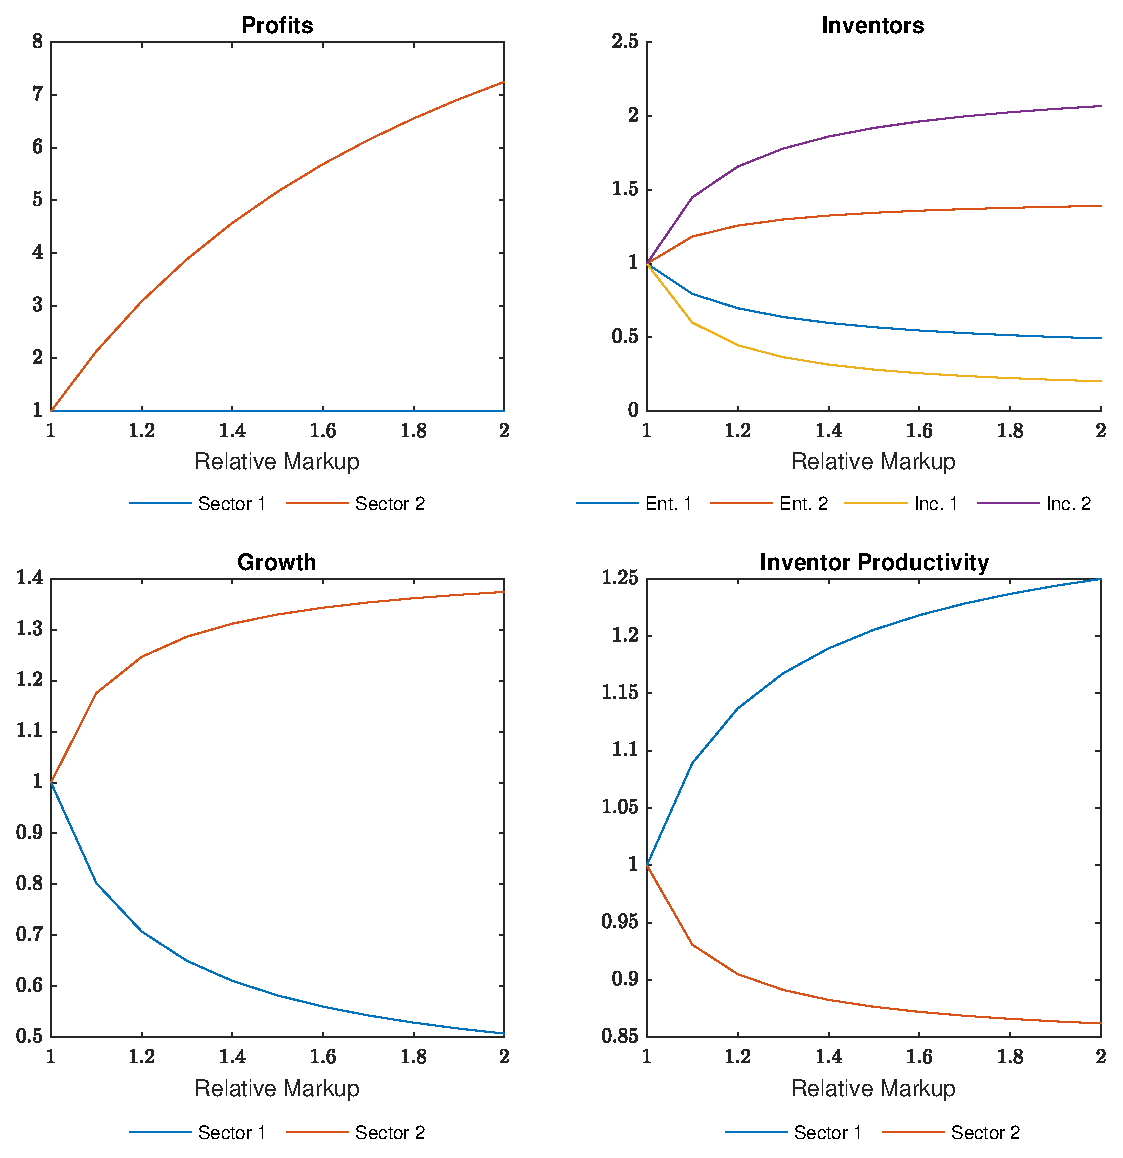
\includegraphics[width=1\textwidth]{graphs/GE_sectors}
\par\end{centering}
\raggedright{}{\small{}Note: This figure reports the comparative statics
for normalized profits, inventors, growth and inventor productivity
in the two-sector model. In all figures, the x-axis reports the markup
of sector 2 relative to sector 1. The parameters used to produce this
Figure are reported in Tables \ref{tab: extPar} and \ref{tab: intPar}.}{\small\par}
\end{figure}
\FloatBarrier

\subsubsection{Growth-Maximizing Policy}

I now turn to solve numerically for the combination of R\&D subsidies
that maximizes growth. I assume that the planner wishes to maximize
growth under a set of different constraint on the instruments available.
In particular, I assume that the planner cannot alter the nature of
innovation, that is, the planner cannot distinguish productive from
unproductive projects, and cannot forbid depositing patents that have
no productive value. In this model, eliminating protection for incumbents
would lead to a first-best where only entrants conduct R\&D, and reallocation
could only be beneficial to growth, as discussed in the previous section. 

I start from the 2012 equilibrium of my model economy, where the gap
in markups between sector 2 and sector 1 is 20\%, and all firms receive
a $19\%$ subsidy to inventors' wages and a 23\% tax on profits. I
then evaluate numerically three cost-neutral alternatives relative
to this benchmark, that is, I constrain the planner to leave the expenditure
on R\&D subsidies as a percentage of GDP fixed at the 2012 benchmark.
In the first scenario, the planner is allowed to distribute subsidies
freely, and can condition their reception on both the state of the
market (protected or unprotected) and the identity of the receiving
firm (entrant or incumbent). In the other two scenarios, I only allow
the planner to act on one of these dimensions at a time. That is,
the planner can either control the cross-sector distribution of funds,
but not the allocation across incumbents and entrants, or vice versa. 

The results of this exercise are presented in Table \ref{tab: Policy}.
The 2012 equilibrium is reported in Columns 1 and 2. For reference,
the 1997 calibrated model has two identical sectors, that share the
stock of inventors equally, and within each sector incumbents have
30.3\% of the overall inventors employed, and GDP growth is 3\% per
annum, as reported in Table \ref{tab: intPar}. In the 2012 baseline,
the distribution of inventors is tilted towards the second sector,
where markups have increased, which results in a fall in annual GDP
growth of .07pp, about 2.5\% of the 1997 benchmark. As shown in the
graphs above, this new equilibrium sees a larger share of inventors
allocated to incumbents in the second sectors, which increases its
growth relative to its more competitive counterpart, and sees a decline
in productivity resulting from higher defensive innovation. Column
3 and 4 report the optimal cost-neutral R\&D subsidies chosen by a
growth-maximizing planner. Somewhat surprisingly, the most efficient
allocation of funds turns out to be an entry subsidy to entrants in
the more concentrated sector only. However, this result can be easily
rationalized through the findings in Figure \ref{fig:TwoSecSectors}.
As discussed above, the outflow of inventors from sector 1 increases
inventor productivity due to reduced defensive innovation. It is therefore
more efficient to leave entry unchanged in sector 1, and act directly
on the inventors' misallocation occurring in sector 2. This intuition
is confirmed by the results for the scenario in which the planner
can only allocate R\&D subsidy to one of the sector, but cannot condition
on the identity of the firm. In this case, subsidies are in part used
to increase incumbents' defensive innovation, which is also made more
attractive by the overall increase in entry. While this policy does
allow the planner to recover most of the lost ground relative to the
1997 equilibrium, bringing growth up to 2.99\%, it is still not as
effective as alternative cost-equivalent policies. In particular,
an alternative that might be easily implementable is a blanket entry
subsidy as reported in Columns 6 and 7, which achieves a growth in
annual output of 3.38\%, which is above the starting 1997 equilibrium. 

To conclude, the policy analysis suggests that entry subsidies are
the most effective policy to contrast the friction introduced by defensive
innovation in this model economy. In particular, it is best to subsidize
entrants in less competitive sectors, where this friction is most
pronounced, which increases growth by 0.5pp per annum. A more feasible
uniform R\&D subsidy to entrants produces quantitatively similar effects.
Conversely, sector-specific subsidies to reallocate inventors to more
competitive sectors are less effective, since they get channeled to
incumbents who employ them to conduct pre-emptive innovation, precisely
the source of inefficiency that the planner wishes to contrast.

\begin{sidewaystable}

\caption{Comparison of R\&D Policies in the Two-Sector Model}
\label{tab: Policy}
\begin{centering}
\begin{tabular}{l  <{\onslide<1->}d<{\onslide<1->}d<{\onslide<2->} HH d<{\onslide<2->}d<{\onslide<4->}d<{\onslide<4->}d<{\onslide<5->}d<{\onslide<5->} d<{\onslide}}
& \multicolumn{2}{c}{Baseline} &	\multicolumn{2}{H}{Optimal Subsidies} & \multicolumn{2}{c}{Optimal Cost-Neutral} & \multicolumn{2}{c}{Cost-Neutral Sector}  & \multicolumn{2}{c}{Cost-Neutral Entry}  \\
\midrule
&Sector \ 1 & Sector \ 2 & Sector \ 1 & Sector \ 2 & Sector \ 1 & Sector \ 2 & Sector \ 1 & Sector \ 2 & Sector \ 1 &Sector \ 2 \\ 
&(1)&(2)&(3)&(4)&(3)&(4)&(5)&(6)&(7)&(8)\\ \midrule 
\textsl{R\&D Subsidies:} \\ 
%$\tau$ & $23\%$ & $23\%$ & $23\%$ & $23\%$ & $23\%$ & $23\%$ & $23\%$ & $23\%$ & $23\%$ & $23\%$ \\ 
$s_{I}$ &\marktopleft{b1} $19\%$ & $19\%$ & $0\%$ & $0\%$ & \marktopleft{b3}$0\%$ & $0\%$ &  \marktopleft{b8}$46.17\%$ & $0\%$ & $0\%$ & $0\%$  \\ 
$s_e$ & $19\%$ & $19\%$ \markbottomright{b1}{red} & $1\%$ & $75.39\%$ & $0\%$ & $41.78\%$ \markbottomright{b3}{red} & $46.17\%$ & $0\%$ \markbottomright{b8}{red}&\marktopleft{b12} $29\%$ & $29\%$   \markbottomright{b12}{red} \\ 
\\[-.2cm]
\textsl{Aggregates:}\\ 
$L^{RD}_{I}$ &\marktopleft{b10} $6.70$ & \marktopleft{b5} $24.87$ & $24.87$ & $4.47$ & $6.37$ & \marktopleft{b6} $15.95$ &\marktopleft{b7} $10.83$ & $19.51$ & $4.83$ & $18.45$ \\ 
$L^{RD}_{e}$ & $24.41$  \markbottomright{b10}{red} & $44.02$ \markbottomright{b5}{red} & $23.12$ & $66.57$ & $23.87$ & $53.81$\markbottomright{b6}{red}& $30.24$ \markbottomright{b7}{red}& $39.42$ & $27.41$ & $49.30$ \\ 
$L^{RD}_{TOT}$ &\marktopleft{b2} $31.11$ & $68.89$ & $28.96$ &  $71.04$ &\marktopleft{b4} $30.25$ & $69.75$ & $41.07$ & $58.93$ & $32.25$ & $67.75$ \\ 
Sector Growth $2.12\%$ & $3.74\%$ & & &  & $2.08\%$ & $4.78\%$ & $2.61\%$ & $3.36\%$ & $2.45\%$ & $4.31\%$ \\ 
\midrule
GDP Growth &  \multicolumn{2}{c}{\onslide<1->{\marktopleft{b11}$2.93\%$}}  \markbottomright{b2}{red}  & \multicolumn{2}{H}{$3.15\%$} & \multicolumn{2}{c}{\onslide<2-> \marktopleft{b14}$3.43\%$} \markbottomright{b4}{red}   & \multicolumn{2}{c}{\onslide<4-> \marktopleft{b9} $2.99\%$} \markbottomright{b9}{red}& \multicolumn{2}{c}{\onslide<5-> \marktopleft{b13} $3.38\%$} {\onslide<1->} \markbottomright{b13}{red} \\ \hline %
%Subsidy/GDP & $0.20\%$ & $0.36\%$ & $0\%$ & $1.66\%$ & $0\%$ & $0.56\%$ & $0.55\%$ & $0\%$ & $0.22\%$ & $0.34\%$ \\ 
%Revenue/GDP & $1.02\%$ & $2.32\%$ & $1.02\%$ & $2.32\%$ & $1.02\%$ & $2.32\%$ & $1.02\%$ & $2.32\%$ & $1.02\%$ & $2.32\%$ \\ 

\end{tabular}
\uncover<1-2>{\tikz[overlay,remember picture,inner sep=1pt] \node[draw=red,rounded corners,fit=(marker-b1-a.north west) (marker-b1-b.south east)] {};}
\uncover<1-2>{\tikz[overlay,remember picture,inner sep=1pt] \node[draw=red,rounded corners,fit=(marker-b2-a.north west) (marker-b2-b.south east)] {};}
\uncover<2>{\tikz[overlay,remember picture,inner sep=1pt] \node[draw=red,rounded corners,fit=(marker-b3-a.north west) (marker-b3-b.south east)] {};}
\uncover<2>{\tikz[overlay,remember picture,inner sep=1pt] \node[draw=red,rounded corners,fit=(marker-b4-a.north west) (marker-b4-b.south east)] {};}
\uncover<3>{\tikz[overlay,remember picture,inner sep=1pt] \node[draw=red,rounded corners,fit=(marker-b5-a.north west) (marker-b5-b.south east)] {};}
\uncover<3>{\tikz[overlay,remember picture,inner sep=1pt] \node[draw=red,rounded corners,fit=(marker-b6-a.north west) (marker-b6-b.south east)] {};}
\uncover<4>{\tikz[overlay,remember picture,inner sep=1pt] \node[draw=red,rounded corners,fit=(marker-b7-a.north west) (marker-b7-b.south east)] {};}
\uncover<4>{\tikz[overlay,remember picture,inner sep=1pt] \node[draw=red,rounded corners,fit=(marker-b8-a.north west) (marker-b8-b.south east)] {};}
\uncover<4>{\tikz[overlay,remember picture,inner sep=1pt] \node[draw=red,rounded corners,fit=(marker-b9-a.north west) (marker-b9-b.south east)] {};}
\uncover<4>{\tikz[overlay,remember picture,inner sep=1pt] \node[draw=red,rounded corners,fit=(marker-b10-a.north west) (marker-b10-b.south east)] {};}
\uncover<4>{\tikz[overlay,remember picture,inner sep=1pt] \node[draw=red,rounded corners,fit=(marker-b11-a.north west) (marker-b2-b.south east)] {};}

\uncover<5-6>{\tikz[overlay,remember picture,inner sep=1pt] \node[draw=red,rounded corners,fit=(marker-b12-a.north west) (marker-b12-b.south east)] {};}
\uncover<5-6>{\tikz[overlay,remember picture,inner sep=1pt] \node[draw=red,rounded corners,fit=(marker-b13-a.north west) (marker-b13-b.south east)] {};}
\uncover<6>{\tikz[overlay,remember picture,inner sep=1pt] \node[draw=red,rounded corners,fit=(marker-b14-a.north west) (marker-b4-b.south east)] {};}
\uncover<6>{\tikz[overlay,remember picture,inner sep=1pt] \node[draw=red,rounded corners,fit=(marker-b11-a.north west) (marker-b2-b.south east)] {};}\\
\par\end{centering}
\raggedright{}{\small{}Note: The figures reported in this Table give
the optimal allocation of R\&D subsidies and the resulting aggregate
outcomes for a planner wishing to maximize aggregate growth in the
economy. The column headings refer to the various scenarios described
above. ``Baseline'' refers to the subsidy allocation reflecting
the 2012 equilibrium, where subsidies do not condition on sectors
or the position of firms within sectors; ``Optimal Cost-Neutral''
refer to the scenario where the planner is allowed to freely allocate
R\&D subsidies subject to the constraint that overall R\&D subsidy
expenditure as a percentage of GDP is held fixed at its 2012 benchmark;
``Cost-Neutral Sector'' consider a scenario where the planner can
choose which sector to allocate funds to, but not which firms within
the sector should receive the subsidy; ``Cost-Neutral Entry'' computes
the optimal universal entry subsidy, under the assumption that the
planner cannot condition its reception on the sector firms operate
in. }{\small\par}
\end{sidewaystable}



\section{Conclusion and Future Work\label{sec:Conclusion}}

In this paper, I have proposed and documented a novel explanation
for the observed decline in growth and R\&D productivity over the
last few decades. 

My empirical results showed that increasing misallocation of inventors
across different product markets can account for up to $27\%$ of
the observed decline in output per worker growth in the sectors I
analyze. This misallocation resulted from uneven increases in concentration
across product markets, which were accompanied by an increase in the
share of inventors accruing to less competitive sectors. I interpret
my findings as resulting from an increase in defensive innovation
in concentrated sectors, defined as R\&D activities conducted with
the primary aim of blocking further entry, which manifest in the data
as a fall in patents' forward citations and an increased share of
inventors employed by the largest incumbents in these sectors.

The theoretical analysis examined the effects of defensive innovation
in a Schumpeterian model of creative destruction, where incumbents
can conduct defensive innovation to raise new entrants' costs. In
the model, pre-emptive innovation is crucial to generate misallocation
across sectors, which would not occur in the absence of this mechanism.
Having established the importance of this channel, I employed a calibrated
two-sector version of the model to study the growth-maximizing allocation
of R\&D subsidies across sectors, as well as between incumbents and
entrants. My analysis suggests that R\&D subsidies provided to entrants
constitute the most effective policy, directly tackling the friction
generated by defensive innovation, and can increase growth by up to
17\% of my baseline (0.5pp in absolute terms).

Two main directions for future research stand out. First, it would
be important to investigate the validity of my findings to an international
context. Indeed, many findings in the literature of competition and
innovation depend strongly on the country and the period analyzed.
Second, my paper highlights the role of pre-emptive innovation as
a major driver of the fall in R\&D productivity. However, this topic
is still relatively under-explored, and a thorough investigation of
the evolution, causes and consequences of this phenomenon seems highly
relevant in view of my results. 

\newpage{}

\bibliographystyle{abbrvnat}
\phantomsection\addcontentsline{toc}{section}{\refname}\bibliography{bibliography/Bibliography}
\newpage{}


\appendix

\section{Data Construction Details\label{app: Data-Construction-Details}}

\subsection{Knowledge Markets}

\paragraph{Rescaling Inventor Flows}

As explained in the main text, the measure of inventor flows aims
to capture the strength of the connections between two sectors. I
take several steps to ensure that I do not overestimate these connections
and to normalize them to account for the size of sending and receiving
sectors. 

As a first step, I build normalized directed flows for each inventor
$i$ in order to avoid double counting. For example, for transitions
between sector $1$ and $2$, I define:

\begin{align*}
\text{flow}_{1\rightarrow2,i,t} & \equiv\frac{\sum\text{\ensuremath{\bm{1}\left\{ i\text{ moves }1\rightarrow2\text{ in }t\right\} }}}{\sum_{j,k}\text{\ensuremath{\bm{1}\left\{ i\text{ moves }j\rightarrow k\text{ in }t\right\} }}}\times\alpha_{i}.
\end{align*}
This measure attributes a fraction of the effective inventor fixed
effect $\alpha_{i}$ to each transition in proportion to the number
of overall inventor $i$'s transitions across sectors in each year.
The first term in this formula is precisely the share of transitions
from sector $1$ to sector $2$ relative to overall transitions between
any two sectors $j$ and $k$ that inventor $i$ took part in.

Second, I compute total inflows (outflows) for each NAICS 4-digit
sector, summing over all years, inventors and origin (destination)
sectors. For example, inflows for sector $1$are defined as:
\[
\text{inflow}_{1}=\sum_{n}\sum_{t}\sum_{i}\text{flow}{}_{n\rightarrow\text{1},i,t},
\]
where $n$ denotes origin NAICS sectors, $t$ years, and $i$ inventor
identifiers. 

Third, I proceed to compute the share of directed flows between each
pair of sector as a share of total inflows or outflows. For example,
the share of inflows coming from sector $2$ and entering sector $1$
is defined as:
\[
\text{share}_{1\ensuremath{\leftarrow}2}=\frac{\sum_{t}\sum_{i}\text{flow}_{2\rightarrow1,i,t}}{\text{inflow}_{1}}.
\]
 In this example, this measure captures the relative importance of
inflows from sector $2$ for the overall number of inventors received
by sector $1$. However, this measure can still overstate flows from
large to small sectors, or vice versa. As a result, and since I need
undirected flows to apply the Louvain algorithm, I define network
edge weights starting from an average of the above shares of inflows
and outflows for each sector and taking the minimum between the two
measures as follows:

\begin{align*}
W_{12}=W_{21}=\min & \left\lbrace \frac{\text{share}_{\text{1\ensuremath{\leftarrow}2}}+\text{share}_{\text{1\ensuremath{\rightarrow}2}}}{2},\right.\\
 & \left.\frac{\text{share}_{\text{1\ensuremath{\leftarrow}2}}+\text{share}_{\text{1\ensuremath{\rightarrow}2}}}{2}\right\rbrace ,
\end{align*}
where $W_{12}=W_{21}$ since the final network is undirected.

\paragraph{Modularity Maximization Formula and Algorithm}

In order to identify knowledge markets from the network constructed
above, I employ the Louvain community detection algorithm \citep{blondelFastUnfoldingCommunities2008}.
This algorithm maximizes the modularity of the network, $Q$, assigning
each sector $i$ to one of $N$ \emph{non-overlapping }communities
$c$. Accordingly, the objective function for this problem is given
by:
\[
\max_{N}\max_{\left(c_{1},\dots,c_{N}\right)}Q\equiv\frac{1}{2\bm{W}}\sum_{ij}\left[W_{ij}-\frac{\bm{W}_{i}\bm{W}_{j}}{2\bm{W}}\right]\bm{1}\left\{ c_{i}=c_{j}\right\} ,
\]
where $W_{ij}$, weight of the edge connecting node $i$ to $j$,
and bold variables denote other summations for ease of notation. In
particular, I define $\bm{W_{i}}\equiv\sum_{k}\sum_{i}W_{ik},$ as
the sum of weights for edges with one end in node $i$, and the sum
of all weights in the network, respectively. The indicator $\bm{1}\left\{ c_{i}=c_{j}\right\} $
takes a value of 1 when nodes $i$ and $j$ belong to the same community.
Note that the maximization is carried out both over the number of
communities and the assignment of nodes to each community. This measure
can be interpreted considering that $\frac{\bm{W}_{i}\bm{W}_{j}}{2\bm{W}}$,
is the expected number of edges that arise between nodes $i$ and
$j$ in a random network. Therefore, modularity maximizes the distance
between the density of linkages within communities $W_{ij}$ relative
to the overall density of links that would arise randomly.

Since looping over all the permutations of nodes and community is
numerically unfeasible, the Louvain algorithm follows an iterative
procedure to maximize modularity. First, it assigns each node to its
own community. Then, it repeats iteratively the following three steps:
\begin{enumerate}
\item Compute local deviations in modularity from reassigning the node to
neighboring communities;
\item Assign nodes to communities following the local improvement granting
the highest modularity increase;
\item Redefine a network with new communities as nodes.
\end{enumerate}
These steps are repeated until there is no significant improvement
in modularity for further steps.


\section{Additional Results and Robustness \label{app: Additional-Results-Rob}}


\subsection{Results on Overall Inventor Shares}

Table \ref{tab: RegTotShare} reports the effect of concentration
increases on the share of inventors across all knowledge markets.
While the correlation is positive and significant when some outliers
are removed, this relation is not robust to the inclusion of all observations
or the the alternative trimming procedure provided by the Mahalanobis
distance. This result is unsurprising in light fo two points discussed
in the main text. First, as highlighted in Section \ref{subsec:KnowledgeMarkets},
if ordinary flows of inventors across unrelated sectors are small
or absent, we should not expect any effect of changes in these sectors'
characteristics on the distribution of inventors. Second, the findings
reported in Table \ref{tab: RegShInvHHI} suggest that cross-knowledge-market
flows are not significant, as apparent from a comparison of specifications
with and without knowledge-market fixed effects. The results presented
in this section therefore speak to the importance of accurately delineating
labor markets for inventors when assessing their flows across product
markets.

\begin{table}[h]
\caption{Regressions of Change in Total Inventors' Share over Change in HHI
Lower Bound, Long-Difference, 1997-2012\label{tab: RegTotShare}}

\begin{centering}
\scalebox{.7}{{
\def\sym#1{\ifmmode^{#1}\else\(^{#1}\)\fi}
\begin{tabular}{l*{6}{c}}
\hline\hline
                    &$\Delta$ Total Inventor Share (pp)   &               &               &               &               &               \\
                    &\multicolumn{1}{c}{(1)}   &\multicolumn{1}{c}{(2)}   &\multicolumn{1}{c}{(3)}   &\multicolumn{1}{c}{(4)}   &\multicolumn{1}{c}{(5)}   &\multicolumn{1}{c}{(6)}   \\
\hline
$\Delta \underline{\text{HHI}}$&       0.297   &       1.692   &       1.328*  &       1.532*  &       0.271   &       1.889   \\
                    &     (2.007)   &     (1.956)   &     (0.649)   &     (0.696)   &     (2.038)   &     (2.023)   \\
$\Delta \log$ Sales &       0.460   &       0.436   &       0.133** &       0.109*  &       0.464   &       0.472   \\
                    &     (0.281)   &     (0.292)   &     (0.047)   &     (0.047)   &     (0.283)   &     (0.312)   \\
\hline
Knowledge Market FE &               &   \ding{51}   &               &   \ding{51}   &               &   \ding{51}   \\
Sample              & Full    & Full    &Trimmed   &Trimmed  &Mahalanobis  &Mahalanobis   \\
Weight              &       Sales   &       Sales   &       Sales   &       Sales   &       Sales   &       Sales   \\
Observations        &         157   &         153   &         147   &         143   &         150   &         139   \\
\hline\hline
\end{tabular}
}
}\\
\par\end{centering}
\raggedright{}{\small{}Note: Regressions weighted by sales in 2012;
Robust standard errors in parentheses; Symbols denote significance
levels $\left(+\ p<0.1,^{*}\ p<0.05,^{**}\ p<.01,^{***}\ p<.001\right)$;
Checkmarks indicate the inclusion of fixed effects. Please refer to
notes in Table \ref{tab: RegShInvHHI} for further details.}{\small\par}
\end{table}


\subsection{Using the Raw Number of Inventors instead of Fixed-Effects\label{app: Using-N-inv}}

This Appendix reports the results for the main analysis presented
in Section \ref{subsec:MainResults} using the raw number of total
inventors instead of the fixed effects from regression (\ref{eq:one-1-1}),
which might be inconsistently estimated. The following Tables, to
be compared with Tables \ref{tab: RegShInvNoctrl} and \ref{tab: RegShInvHHI}
in the main text, show that the results are qualitatively unchanged.
Looking at the scale of the y-axis in panel (a) of Figure \ref{fig: scattersDksh-1},
it is apparent that the shares of the raw number of inventors are
more volatile, and presents larger changes. This is easily explained
by the fact that differences in research requirements across patent
classes, firms and years are not absorbed as in the effective inventor
measure. This greater variability simply results in larger and noisier
coefficients, which nevertheless remain positive and significant.
\begin{sidewaystable}
\caption{Regressions of Change in 4-digit Knowledge Market Share of Total Inventors
over Change in HHI Measures, Long-Differences, 1997-2012\label{tab: RegShInvNoctrl-1-1}}

\begin{centering}
\scalebox{.9}{\input{\string"/Users/andreamanera/Dropbox (MIT)/Research/ProductInnovation/docs/JMP/draft/tab/Dk4_sh_inv_hhi_noctrl_N_inv.tex\string"}}\\
\par\end{centering}
\raggedright{}{\small{}Note: Regressions weighted by sales in 2012;
Robust standard errors in parentheses; Symbols denote significance
levels $\left(+\ p<0.1,^{*}\ p<0.05,^{**}\ p<.01,^{***}\ p<.001\right)$;
Checkmarks indicate the inclusion of fixed effects. This Tables presents
the results of specifications (\ref{eq: spec}), when the outcome
is the share of total inventors of sector $p$ over total inventors
in knowledge market $k$, and the independent variable is the change
in the lower bound of the Herfindal-Hirschman Index for product market
$p$, as implied by Economic Census concentration ratios, or the HHI
index reported in the Economic Census. ``Full Sample'', ``Trim
Outliers'' and ``Mahalanobis 5\%'' refer to the samples described
in the main text.}{\small\par}
\end{sidewaystable}
\begin{sidewaystable}
\caption{Regressions of Change in 4-digit Knowledge Market Share of Total Inventors
over Change in HHI Lower Bound, Long-Differences, 1997-2012\label{tab: RegShInvHHI-1}}

\begin{centering}
\subfloat[Controlling for Change in Log Real Sales]{\begin{centering}
\par\end{centering}
\centering{}\scalebox{.9}{{
\def\sym#1{\ifmmode^{#1}\else\(^{#1}\)\fi}
\begin{tabular}{l*{6}{c}}
\hline\hline
                    &Ch. 4d K.M. Eff. Inv. Share (\%)   &               &               &               &               &               \\
                    &\multicolumn{1}{c}{(1)}   &\multicolumn{1}{c}{(2)}   &\multicolumn{1}{c}{(3)}   &\multicolumn{1}{c}{(4)}   &\multicolumn{1}{c}{(5)}   &\multicolumn{1}{c}{(6)}   \\
\hline
Ch. HHI lower bound &      71.724+  &      67.160+  &      72.123+  &      67.736+  &      71.772+  &      68.398+  \\
                    &    (39.265)   &    (37.176)   &    (39.530)   &    (37.504)   &    (39.316)   &    (37.717)   \\
Ch. Log Real Sales  &       1.864*  &       1.422*  &       1.852*  &       1.402+  &       1.878*  &       1.443+  \\
                    &     (0.766)   &     (0.717)   &     (0.764)   &     (0.712)   &     (0.774)   &     (0.745)   \\
\hline
4D Knowledge Market FE&               &   \ding{51}   &               &   \ding{51}   &               &   \ding{51}   \\
Sample              & Full Sample   & Full Sample   &Trim Outliers   &Trim Outliers   &Mahalanobis 5\%   &Mahalanobis 5\%   \\
Weight              &       Sales   &       Sales   &       Sales   &       Sales   &       Sales   &       Sales   \\
Observations        &         157   &         156   &         156   &         155   &         150   &         142   \\
\hline\hline
\end{tabular}
}
}}
\par\end{centering}

\begin{centering}
\subfloat[Controlling for Change in Log Real Sales per Company]{\centering{}\scalebox{.9}{ {
\def\sym#1{\ifmmode^{#1}\else\(^{#1}\)\fi}
\begin{tabular}{l*{6}{c}}
\hline\hline
                    &$\Delta$ Inventor Share (pp)   &               &               &               &               &               \\
                    &\multicolumn{1}{c}{(1)}   &\multicolumn{1}{c}{(2)}   &\multicolumn{1}{c}{(3)}   &\multicolumn{1}{c}{(4)}   &\multicolumn{1}{c}{(5)}   &\multicolumn{1}{c}{(6)}   \\
\hline
$\Delta \underline{\text{HHI}}$&     104.562*  &      81.339+  &     103.402+  &      82.040+  &     104.355*  &      82.964+  \\
                    &    (51.534)   &    (43.722)   &    (52.824)   &    (43.556)   &    (51.356)   &    (46.147)   \\
$\Delta \log$ Size  &       0.571   &      -0.277   &       0.196   &      -0.515   &       0.571   &      -0.656   \\
                    &     (1.013)   &     (0.809)   &     (0.920)   &     (0.793)   &     (1.048)   &     (1.049)   \\
\hline
Knowledge Market FE &               &   \ding{51}   &               &   \ding{51}   &               &   \ding{51}   \\
Sample              & Full Sample   & Full Sample   &Trim Outliers   &Trim Outliers   &Mahalanobis 5\%   &Mahalanobis 5\%   \\
Weight              &       Sales   &       Sales   &       Sales   &       Sales   &       Sales   &       Sales   \\
Observations        &          81   &          80   &          80   &          79   &          76   &          69   \\
\hline\hline
\end{tabular}
}
}}\\
\par\end{centering}
\raggedright{}{\small{}Note: Regressions weighted by sales in 2012;
Robust standard errors in parentheses; Symbols denote significance
levels $\left(+\ p<0.1,^{*}\ p<0.05,^{**}\ p<.01,^{***}\ p<.001\right)$;
Checkmarks indicate the inclusion of fixed effects. This Tables presents
the results of specifications (\ref{eq: spec}) and (\ref{eq: specFE}),
when the outcome is the share of effective inventors of sector $p$
over total inventors in knowledge market $k$, and the independent
variable is the change in the lower bound of the Herfindal-Hirschman
Index for product market $p$, as implied by Census concentration
ratios. ``Full Sample'', ``Trim Outliers'' and ``Mahalanobis
5\%'' refer to the samples described in the main text.}{\small\par}
\end{sidewaystable}

\begin{figure}
\caption{Residualized Scatter Plots Corresponding to Selected Columns in Table
\ref{tab: RegShInvHHI-1}, Panel (a)\label{fig: scattersDksh-1}}

\subfloat[Raw Scatter Plot, Specification in Column (2)]{\centering{}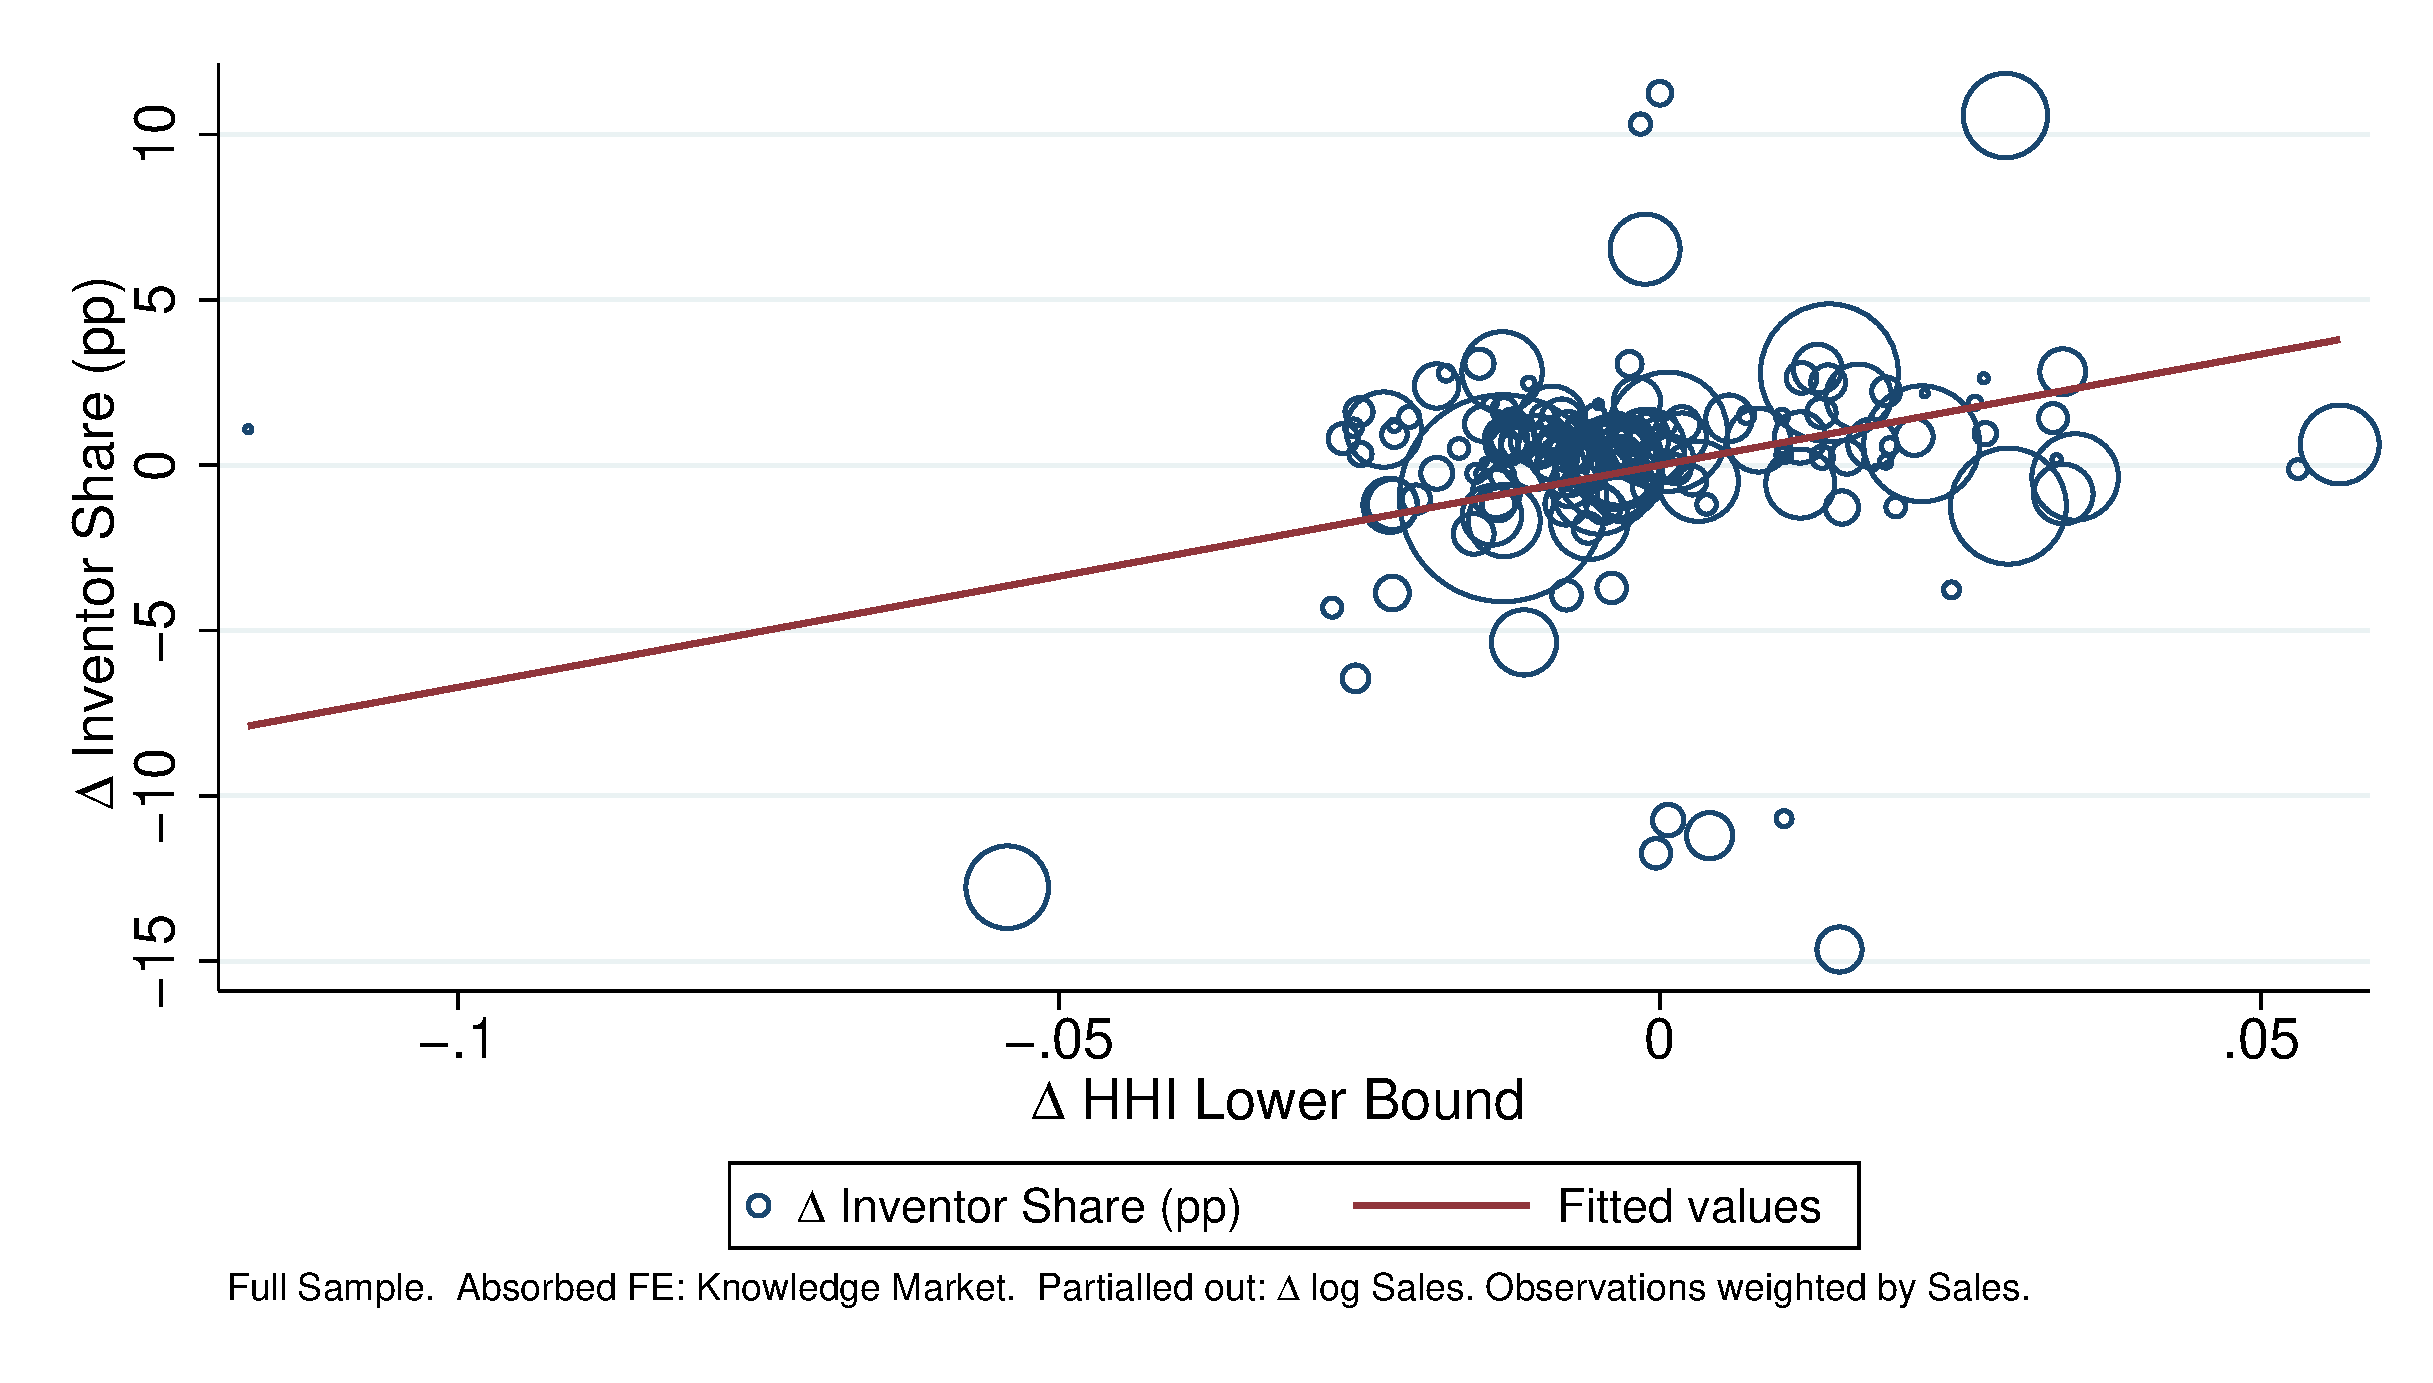
\includegraphics[width=0.9\textwidth]{graphs/raw_Dk4_hhi_N_inv0}}

\subfloat[Binned Scatter Plot, Specification in Column (6)]{\centering{}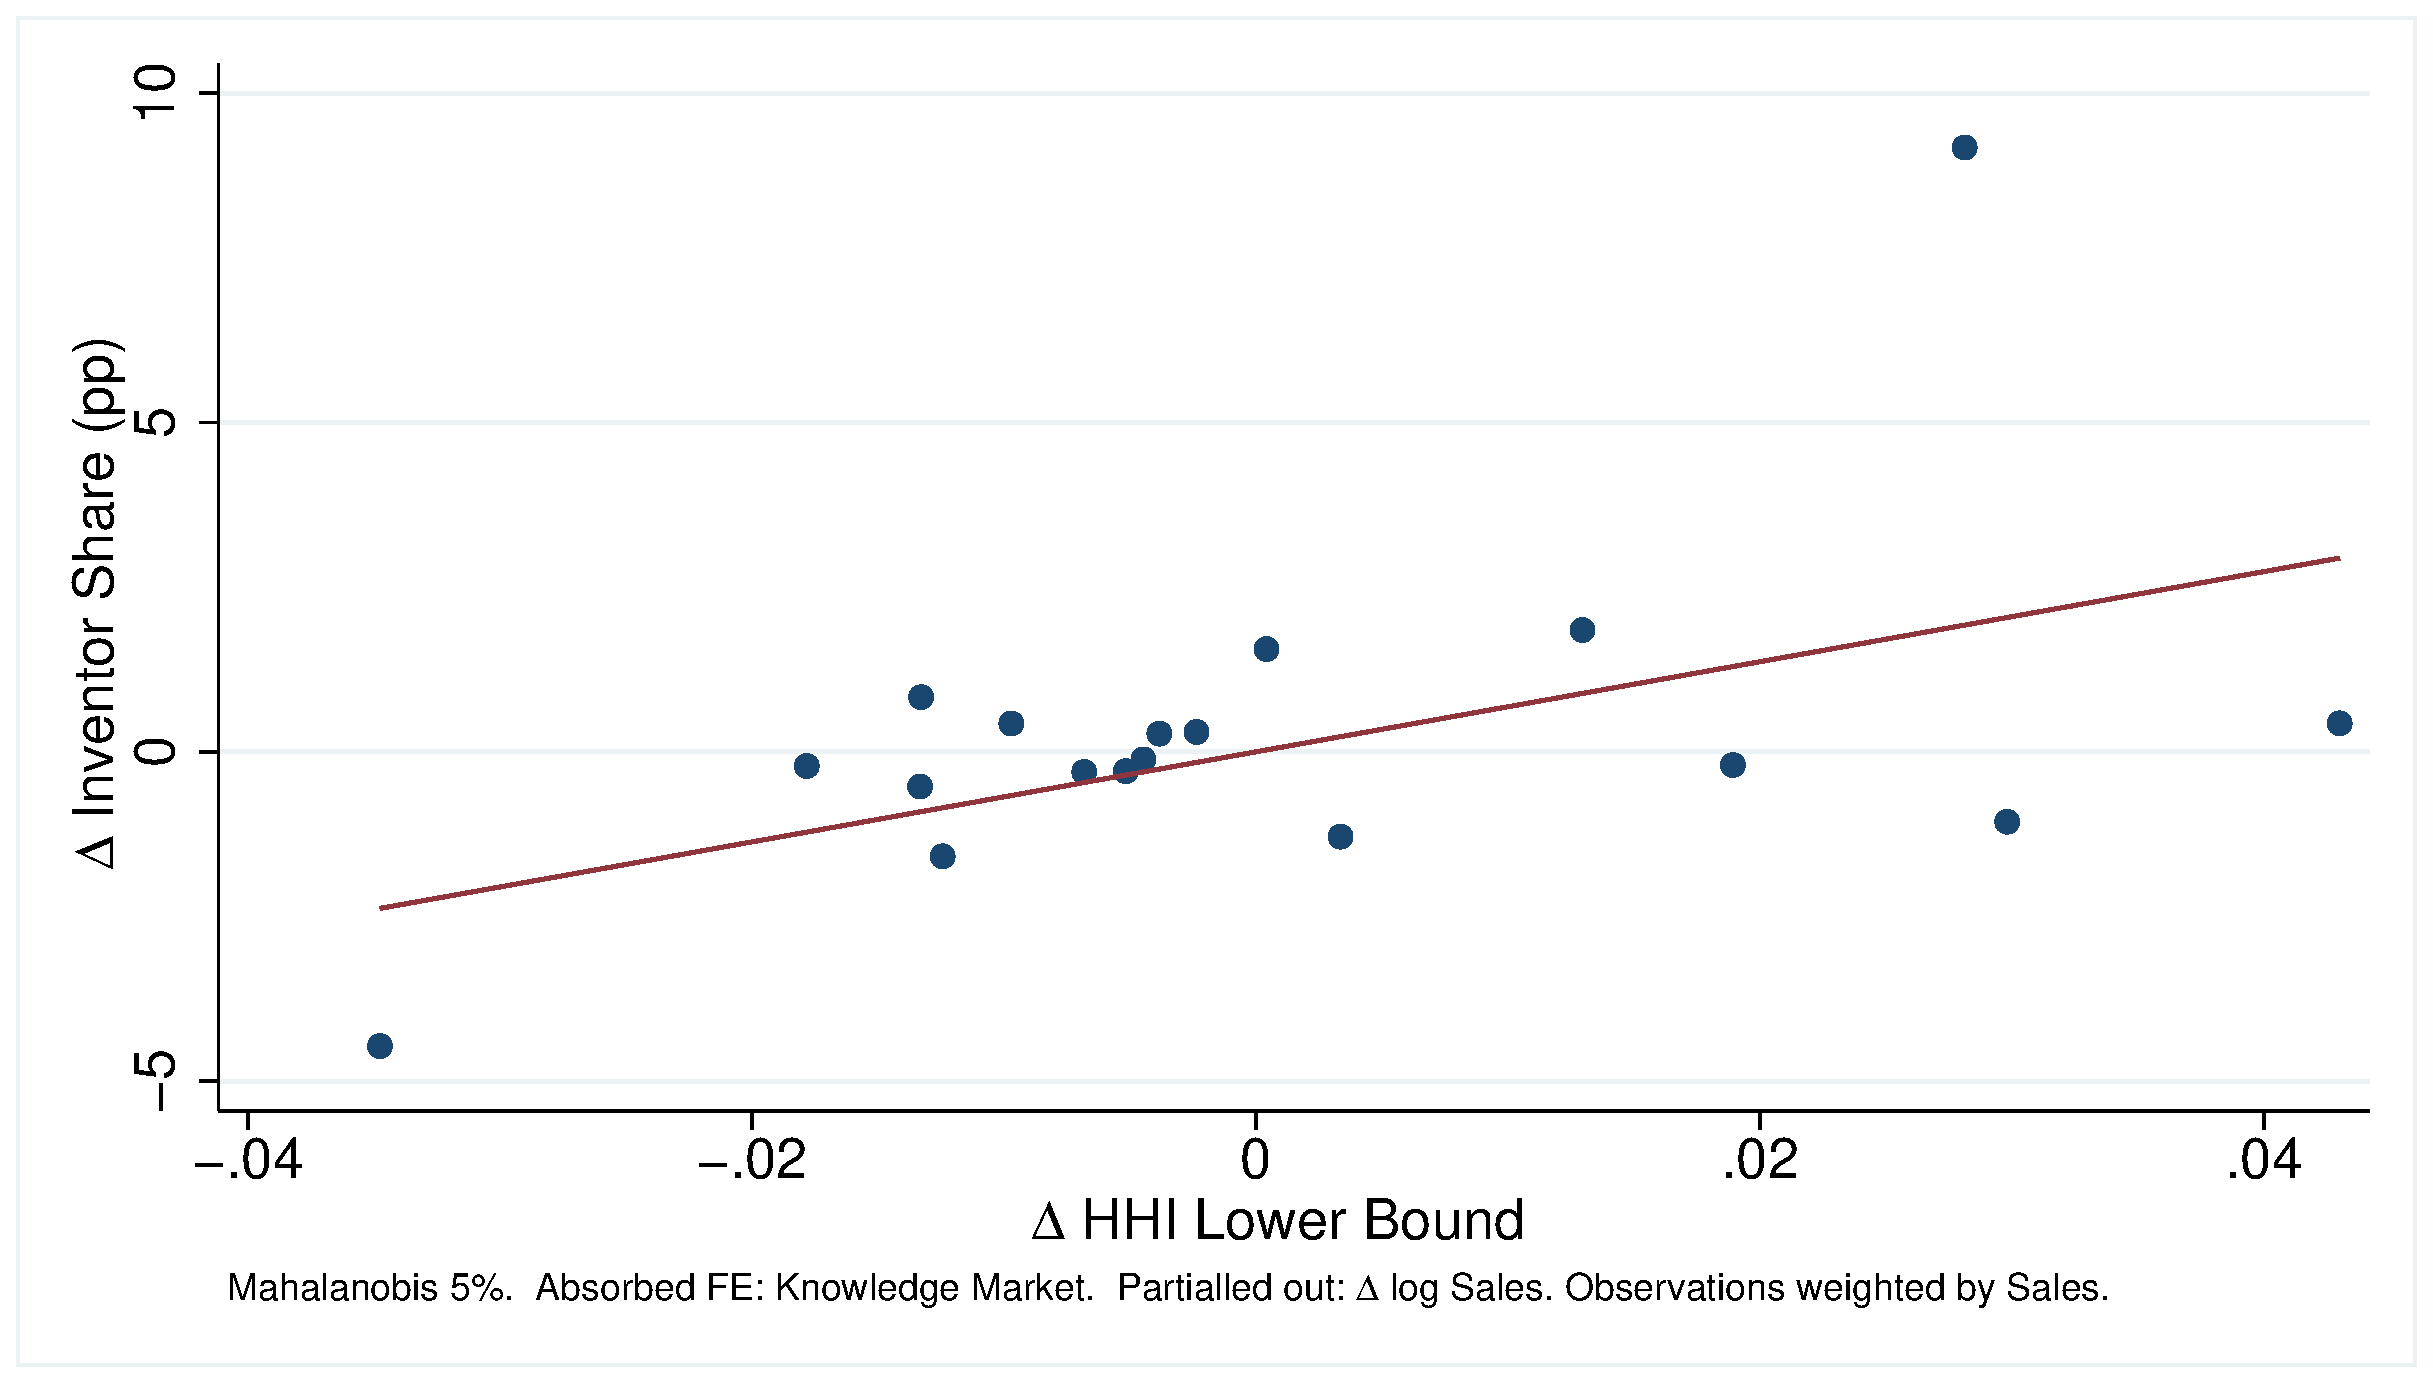
\includegraphics[width=0.9\textwidth]{graphs/bin_Dk4_hhi_N_inv2}}\\

\raggedright{}{\small{}Note: This figure presents residualized scatter
plots of the change in the share of effective inventors of sector
$p$ over total inventors in knowledge market $k$, over the change
in the lower bound of the Herfindal-Hirschman Index for product market
$p$, as implied by Census concentration ratios. The upper panel reports
the data corresponding to the full sample, where both variables have
been residualized by change in log real sales and knowledge market
fixed effects. The size of the markers is proportional to the weight
of each observation in the regression, corresponding to total sector
sales in 2012. The regression line corresponds to the coefficient
on the change in HHI lower bound reported in Column (2) of Table }\ref{tab: RegShInvHHI-1}{\small{}.
The lower panel presents a binned scatter plot on the sample where
the observations with the highest 5\% Mahalanobis distance from sample
centroid have been removed. Observations are aggregated using sales
weights and the regression line results from the specification in
Column (6) of Table }\ref{tab: RegShInvHHI-1}{\small{}.}{\small\par}
\end{figure}
\FloatBarrier

\subsection{Using a Quartic in Sales as Size Control}

This Section displays the results of estimating the specification
in Table \ref{tab: RegShInvHHI} using the changes in the terms of
a fourth-degree polynomial in sales rather than log-sales. This flexible
control specification ensures that my main findings do not rely on
the specific functional form that I assumed above. Table \ref{tab: RegShInvQuartic}
reports the result of this exercise using both effective inventors
(Columns (1) and (2)) and raw inventor counts (Columns (3) and (4))
to compute sector shares. Recall that when using raw inventor counts,
knowledge markets are also constructed according to this measure.
As clear from a comparison of Columns (1) with (2), and (3) with (4),
these two specifications produce statistically undistinguishable results.

\begin{table}[th]
\caption{Regressions of Change in 4-digit Knowledge Market Share of Inventors
over Change in HHI Lower Bound, Long-Differences, 1997-2012\label{tab: RegShInvQuartic}}

\begin{centering}
\scalebox{.9}{\input{\string"/Users/andreamanera/Dropbox (MIT)/Research/ProductInnovation/docs/JMP/draft/tab/Dk4_sh_inv_quartic.tex\string"}}
\par\end{centering}
\raggedright{}{\small{}Note: Regressions weighted by sales in 2012;
Robust standard errors in parentheses; Symbols denote significance
levels $\left(+\ p<0.1,^{*}\ p<0.05,^{**}\ p<.01,^{***}\ p<.001\right)$;
Checkmarks indicate the inclusion of fixed effects. This Tables presents
the results of specifications (\ref{eq: spec}), when the outcome
is the share of effective inventors of sector $p$ over total inventors
in knowledge market $k$, and the independent variable is the change
in the lower bound of the Herfindal-Hirschman Index for product market
$p$, as implied by Census concentration ratios. ``Full Sample''
refers to the sample described in the main text.}{\small\par}
\end{table}


\subsection{Using the HHI as the Independent Variable in Patent Quality Regressions\label{subsec:Patents-with-HHI}}

This Section reports the results analogous to Tables \ref{tab: RegStats}
and \ref{tab: RegFwdCite} in the main text, using the HHI lower bound
as the independent variable rather than the share of inventors. As
should be expected from the high correlation between the two variables,
the results are qualitatively similar to those reported there, with
some distinctions. First, Table \ref{tab: RegStats-1} confirms that
there has a been a large and significant increase in the concentration
of inventors among top firms in product market with increasing HHI.
Differently from the main specification, this seems to be driven primarily
by a fall in the share of the bottom half innovative firms. However,
this does not counter the interpretation provided in the main text
that increased concentration tends to reduce entry, which manifests
in these regressions through a fall in the share of inventors employed
by smaller, and presumably younger, firms. Table \ref{tab: RegFwdCite-1}
shows the robustness of my findings on forward citations to the use
of the HHI as well as weighting the regressions by 2012 sales, although
the generality coefficient appears non-significant, as discussed in
the main text.

\begin{sidewaystable}[ph]
\caption{Regressions of Change in Inventor Distribution Measures over Change
in 4-digit Knowledge Market Share, Long-Difference, 1997-2012\label{tab: RegStats-1}}

\begin{centering}
\scalebox{1}{\input{\string"/Users/andreamanera/Dropbox (MIT)/Research/ProductInnovation/docs/JMP/draft/tab/stats_hhi_inv_fe1.tex\string"}}\\
\par\end{centering}
\raggedright{}{\small{}Note: Regressions weighted by sales in 2012;
Robust standard errors in parentheses; Symbols denote significance
levels $\left(+\ p<0.1,^{*}\ p<0.05,^{**}\ p<.01,^{***}\ p<.001\right)$;
Checkmarks indicate the inclusion of fixed effects. Please refer to
notes in Table \ref{tab: RegShInvHHI} for further details. Column
(1) uses the ratio in the 90 percentile of effective inventors to
the median as the outcome variable. Columns (2) and (3) instead present
the share ratio, that is the share of effective inventors accruing
to the top 10 or 50\% relative to the share accruing to the bottom
50\% of the distribution within each NAICS sector.}{\small\par}
\end{sidewaystable}

\begin{table}
\caption{Regressions of Changes in Forward Citation over HHI Changes, Long-Differences,
1997-2012\label{tab: RegFwdCite-1}}

\begin{centering}
\subfloat[Full sample]{\begin{centering}
\par\end{centering}
\centering{}\scalebox{.9}{\input{\string"/Users/andreamanera/Dropbox (MIT)/Research/ProductInnovation/docs/JMP/draft/tab/fwd_cite_all_hhi_inv_fe1.tex\string"}}}
\par\end{centering}

\begin{centering}
\subfloat[Full sample, restricting to the middle range of the change in inventor
shares ($-2\%$ to $+2\%$)]{\centering{}\scalebox{.9}{ \input{\string"/Users/andreamanera/Dropbox (MIT)/Research/ProductInnovation/docs/JMP/draft/tab/fwd_cite_mid_hhi_inv_fe1.tex\string"}}}\\
\par\end{centering}
\raggedright{}{\small{}Note: Unweighted regressions; Robust standard
errors in parentheses; Symbols denote significance levels $\left(+\ p<0.1,^{*}\ p<0.05,^{**}\ p<.01,^{***}\ p<.001\right)$;
Checkmarks indicate the inclusion of fixed effects. This Tables presents
the results of specification (\ref{eq: specFE}), when the outcome
is the log-change in forward citations and the change in patent generality
in sector $p$ over the change in the share of inventors employed
in sector $p$. Column (1) and (2) presents the results when forward
citations are extrapolated the procedure Hall et al. (2000) to avoid
truncation bias. A specific cite-lag distribution over 35 years is
estimated for each pair of cited and citing CPC2-codes. Column (1)
employs the extrapolation scheme by each pair of CPC2 cited and citing
sector. Column (2) applies the extrapolation scheme to total citations
received by each cited patent. Column (3) presents results on the
patent generality measures. All columns exclude self-citations. Upper
panel: full sample; Bottom panel: excluding sectors with absolute
increase in the inventor share above 2\%.}{\small\par}
\end{table}


\subsection{Using the Lerner Index instead of the HHI\label{app:Using-the-Lerner}}

Following \citet{grullonAreUSIndustries2019a}, I build the Lerner
Index from NBER-CES data for the period 1997-2012 as the ratio:
\begin{equation}
\text{Lerner}_{jt}=\frac{\text{vship}_{jt}-\text{pay}_{jt}-\text{matcost}_{jt}-\text{energy}_{jt}}{\text{vship}_{jt}},\label{eq: Lerner}
\end{equation}
where ``vship'' is the total value of shipments, ``pay'' denotes
total payrolls, ``matcost'' and ``energy'' material and energy
costs, respectively, and $j$ denotes a 6- or 4-digit NAICS sector.
I build two alternative measures, one using 6-digit NAICS sectors,
the original identifier in NBER-CES, and then averaging by sales at
the level of 4-digit NAICS, or first aggregating the revenue and cost
statistics at the level of 4-digit NAICS. Table \ref{tab: LernerVHHI},
shows that the Lerner Index thus constructed is strongly correlated
with the HHI measure used in the main analysis. However, the correlation
is far from perfect, as suggested by the $R^{2}$, suggesting that
this estimate of the Lerner Index might be excessively imprecise.
Indeed, Table \ref{tab: MainWLerner} shows that, when using this
measure instead of the HHI in the main analysis, the coefficients
for the regression of inventors' shares on changes in concentration
stay positive, but become smaller and noisier. This suggests the potential
presence of attenuation bias, a valid concern due to the fact that
the above measure, not based on any structural estimation, can only
imperfectly capture markups. Note that this is also due to the fact
that the Lerner Index is available only for the manufacturing sectors,
which make up about 60\% of the sample, so its use lead to dropping
a substantial amount of observations. When using fitted values from
the regression in Table \ref{tab: LernerVHHI} to extend the measure
to more sectors, as well as reducing the volatility of the series
for available sectors, the coefficients recover magnitudes and significance
close to the baseline presented in \ref{tab: RegShInvHHI}.

\begin{table}[h]
\caption{Regressions of Changes in the Lerner Index over Changes in the HHI
Lower Bound, Long-Difference, 1997-2012\label{tab: LernerVHHI}}

\begin{centering}
\scalebox{1}{{
\def\sym#1{\ifmmode^{#1}\else\(^{#1}\)\fi}
\begin{tabular}{lHc}
\hline\hline
                    &Markup Change 1997-2012, 6d Lerner Index   & $\Delta$ Lerner Index   \\
                    &\multicolumn{1}{H}{(1)}   &\multicolumn{1}{c}{(2)}   \\
\hline
$\Delta \underline{HHI}$&       1.490***&       1.652***\\
                    &     (0.229)   &     (0.257)   \\
\hline
Observations        &         258   &         258   \\
R-squared           &    .1424476   &     .14   \\
\hline\hline
\end{tabular}
}
}\\
\par\end{centering}
\raggedright{}{\small{}Note: Robust standard errors in parentheses;
Symbols denote significance levels $\left(+\ p<0.1,^{*}\ p<0.05,^{**}\ p<.01,^{***}\ p<.001\right)$.
``6d Lerner Index'' refers to the Lerner Index constructed as in
(\ref{eq: Lerner})on NAICS 6-digits averaged at the 4-digit NAICS
level weighting by the value of shipments; ``4d Lerner Index'' is
computed using 4-digit aggregates for the value of shipments, payroll
and costs, summing over the NAICS 6-digit composing each sector. }{\small\par}
\end{table}

\begin{table}[h]
\caption{Regressions of Changes in Inventors' Share over Changes in Actual
and Fitted Lerner Index, Long-Difference, 1997-2012\label{tab: MainWLerner}}

\begin{centering}
{
\def\sym#1{\ifmmode^{#1}\else\(^{#1}\)\fi}
\begin{tabular}{l*{2}{c}}
\hline\hline
                    &Ch. 4d K.M. Eff. Inv. Share (\%)   &               \\
                    &\multicolumn{1}{c}{(1)}   &\multicolumn{1}{c}{(2)}   \\
\hline
Markup Change 1997-2012, 4d Lerner Index&       0.556   &               \\
                    &     (5.465)   &               \\
Fitted Lerner Change&               &      26.736*  \\
                    &               &    (13.363)   \\
\hline
4D Knowledge Market &               &               \\
Sample              & Full Sample   & Full Sample   \\
Weight              &       Sales   &       Sales   \\
Observations        &          81   &         157   \\
\hline\hline
\end{tabular}
}
\\
\par\end{centering}
\raggedright{}{\small{}Note: Robust standard errors in parentheses;
Symbols denote significance levels $\left(+\ p<0.1,^{*}\ p<0.05,^{**}\ p<.01,^{***}\ p<.001\right)$;
Observations weighted by sales. The markup change 1997-2012 is the
long-difference of the Lerner Index described above. ``Fitted Lerner
change'' is the fitted value for the Lerner index based on the estimates
in \ref{tab: LernerVHHI}, and extended to all available sectors in
the main sample. }{\small\par}
\end{table}
\FloatBarrier

\section{Omitted Proofs and Derivations\label{app: Omitted-Proofs}}

\subsection{One-sector model}

\begin{proof}[Proof of Proposition \ref{prop: partialEq}]
 This proof consists of several parts. First, I show that given labor
supplies, output, values and wages grow at the same constant rate,
so the problem can be solved in a steady state of a normalized model.
Second, show that normalized values, $v(\Omega)\equiv V_{t}(\Omega)/Y_{t}$,
are uniquely determined, which gives unique research intensities and
stationary distribution. Third, I derive the stationary distribution
and the expression for growth and inventors' productivity. In what
follows I suppress stars to denote equilibrium quantities for ease
of notation.

Given an endowment, $L$, production labor market clearing in each
period requires:
\[
\int_{0}^{1}l_{i,t}(w)d(i)=L.
\]
That is,
\[
L=\int_{0}^{1}\frac{c_{i,t}}{\phi}y_{i,t}\left(w_{t}\right)d(i)=\frac{1}{\phi}\frac{Y_{t}}{w_{t}},
\]
where the second equality comes from using the demand for output of
product $i$ for $y_{i,t}\left(w_{t}\right)$. This expression immediately
implies that if $Y_{t}$ grows at a constant rate, so does $w_{t}$.
Labor market clearing for R\&D workers reads:
\[
L^{RD}=\zeta\omega x_{e,\omega}\left(\mu_{e,\omega}+\mu_{e,1}\right)+\alpha_{I}\frac{\left(x_{I}\right)^{\gamma}}{\gamma}\mu_{1}.
\]
 In a constant growth equilibrium (CGE), the distribution is stationary,
and since the left hand side is constant, research intensities are
also fixed. A contradiction arises otherwise, since the distribution
is stationary only if research intensities are fixed by the LOM (\ref{eq: StatDist1})-(\ref{eq: statDist4}).
Further, R\&D labor cannot grow since the growth rate in the economy
increases in total R\&D labor for any given distribution, as it will
be clear below. The fact that research intensities are constant immediately
implies, from the optimality of $x_{e,\omega}$, that $V_{t}(1)$
and $w_{t}^{RD}$ grow at the same rate. Indeed, from the FOC for
entrants' research:
\[
0=\mathrm{d}\log x_{e,\omega,t}=\mathrm{d}\log V_{t}(1)-\mathrm{d}\log w_{t}^{RD}.
\]
This result in turn implies, combined with the FOC for $x_{I},$ that
$V_{t}(\omega)$ also grows at the same constant rate. Now consider
the budget constraint of the representative household, combined with
product market clearing, $Y_{t}=C_{t}$: 
\[
r_{t}A_{t}-\dot{A}_{t}+w_{t}^{RD}L^{RD}+w_{t}L=Y_{t},
\]
where $A_{t}$ denote the household's assets, that is all firms in
the economy. Therefore the above reads:
\[
r_{t}\left(\mu_{1}V_{t}(1)+\mu_{\omega}V_{t}(\omega)\right)-\mu_{1}\dot{V}_{t}(1)-\mu_{\omega}\dot{V}_{t}(\omega)+w_{t}^{RD}L^{RD}+w_{t}L=Y_{t}
\]
Dividing both sides by $V(1)$, using the Euler equation and rearranging
we obtain:
\[
\left(g+\rho\right)\left(\mu_{1}+\mu_{\omega}\frac{V_{t}(\omega)}{V_{t}(1)}\right)-\mu_{1}g_{V_{1}}-\mu_{\omega}\frac{V_{t}(\omega)}{V_{t}(1)}g_{V_{1}}+\frac{w_{t}^{RD}}{V_{t}(1)}L^{RD}=\frac{Y_{t}}{V_{t}(1)}-\frac{w_{t}}{V_{t}(1)}L.
\]
By what shown above, all terms on the left hand side are constant
in $t$, since research wages and values grows at the same rate and
the distribution is stationary. Since $Y_{t}$ and $w_{t}$ grow at
the same rate positive rate, it must be that $V_{t}(1)$ also grows
at the same rate as $Y_{t}$. This proves that $g_{V_{1}}=g=g_{c}=g_{w}=g_{w^{RD}}.$

As a result, in a CGE, it is possible to define normalized constant
values, $v(\Omega)\equiv V_{t}(\Omega)/Y_{t}$. The system of equations
defining the recursive problem in this equilibrium reads:
\begin{align}
\rho v(1) & =\max_{x_{I}}\left\{ \left(\frac{\phi-1}{\phi}\right)-\alpha_{I}\frac{x_{I}^{\gamma}}{\gamma}w^{RD}+x_{I}\left(v(\omega)-v(1)\right)-x_{e,1}v(1)\right\} ,\label{eq:normV1}\\
\rho v(\omega) & =\left(\frac{\phi-1}{\phi}\right)+\delta\left(v(1)-v(\omega)\right)-x_{e,\omega}v(\omega),\label{eq:normVom}
\end{align}
where the left hand side comes from using the Euler equation:
\[
r=g+\rho
\]
Which gives 
\[
r\frac{V_{t}(\Omega)}{Y_{t}}-\frac{\dot{V}_{t}(\Omega)}{Y_{t}}\frac{Y_{t}}{\dot{Y}_{t}}\frac{\dot{Y_{t}}}{V_{t}(\Omega)}\frac{V_{t}(\Omega)}{Y_{t}}=\left(\rho+g\right)v(\Omega)-gv(\Omega)=\rho v(\Omega).
\]

I now move to show that normalized values (\ref{eq:normV1}) and (\ref{eq:normVom})
are uniquely determined. Given entrants' decisions, and a wage rate
$w^{RD},$ the incumbent's choice of R\&D satisfies:
\[
x_{I}=\bm{1}\left\{ v(\omega)-v(1)>0\right\} \left(\frac{v(\omega)-v(1)}{\alpha_{I}w^{RD}}\right)^{\frac{1}{\gamma-1}}.
\]
Entrants taking $x_{I}$ as given optimally set:
\[
x_{e,1}=\bm{1}\left\{ v(1)>0\right\} \frac{v(1)}{\zeta w^{RD}},\quad x_{e,\omega}=\bm{1}\left\{ v(1)>0\right\} \frac{v(1)}{\zeta\omega w^{RD}}.
\]
Note that these solutions immediately imply that the normalized value,
$v(1)$, is strictly positive. Indeed, $v(1)<0$ would imply:
\[
\rho v(1)=\pi+\bm{1}\left\{ v(\omega)-v(1)>0\right\} \left(\frac{\gamma-1}{\gamma}\left(\frac{v(\omega)-v(1)}{\alpha_{I}w^{RD}}\right)^{\frac{1}{\gamma-1}}\right)\left(v(\omega)-v(1)\right)
\]
where the right hand side is strictly positive. Plugging optimal solutions
into the system of equations determining the value functions (\ref{eq: normV1})
and (\ref{eq: normV2}) gives:
\begin{align}
\rho v(1)-\pi-\bm{1}\left\{ v(\omega)-v(1)>0\right\} \left(\frac{\gamma-1}{\gamma}\left(\frac{v(\omega)-v(1)}{\alpha_{I}w^{RD}}\right)^{\frac{1}{\gamma-1}}\right)\left(v(\omega)-v(1)\right)+\frac{v(1)^{2}}{\zeta w^{RD}} & =0\label{eq: sys1-3}\\
\rho v(\omega)-\pi-\delta\left(v(1)-v(\omega)\right)+\frac{v(1)}{\zeta w^{RD}\omega}v(\omega) & =0.\label{eq: sys2-3}
\end{align}
The second equation gives $v(\omega)$ as the following function of
$v(1):$
\[
v(\omega)=\frac{\pi+\delta v(1)}{\rho+\delta+\frac{v(1)}{\zeta w^{RD}\omega}}.
\]

Suppose first that $v(\omega)<v(1).$ In this case, the first equation
gives:
\[
\rho v(1)+\frac{v(1)^{2}}{\zeta w^{RD}}-\pi=0.
\]
The roots of this equation are:
\[
v_{1,2}=\frac{-\rho\pm\sqrt{\rho^{2}+4\frac{\pi}{\zeta w^{RD}}}}{\frac{2}{\zeta w^{RD}}}.
\]
Since the term under the root is strictly positive, only one of these
roots is admissible, so the above system is solved for a unique pair
$v(1),v(\omega).$ Consider now the case $v(\omega)>v(1).$ It is
straightforward to note that $v(\omega)-v(1)$ is decreasing in $v(1).$
This implies that, when rewriting (\ref{eq: sys1-3}) as
\begin{equation}
-\left(\frac{\gamma-1}{\gamma}\left(\frac{v(\omega)-v(1)}{\alpha_{I}w^{RD}}\right)^{\frac{1}{\gamma-1}}\right)\left(v(\omega)-v(1)\right)=\pi-\rho v(1)-\frac{v^{2}(1)}{\zeta w^{RD}},\label{eq:solV1}
\end{equation}
the left hand side is monotonically increasing in $v(1)$, while the
right hand side is monotonically decreasing in $v(1)$. Further, at
$v(1)=0$, the left hand side is strictly negative, while the right
hand side equals $\pi$, while for $v(1)\rightarrow\infty$, the right
hand side tends to $+\infty$ while the left hand side decreases towards
$-\infty$. As a result, (\ref{eq:solV1}) has a unique positive solution. 

The uniqueness of $v(1)$ immediately implies unique $v(\omega)$
and R\&D choices. Given these R\&D choices, the stationary distribution
satisfies 
\begin{align}
0 & =-\left(x_{I}+x_{e,1}\right)\mu_{1}+\delta\mu_{\omega}+x_{e,\omega}\mu_{e,\omega}+x_{e,1}\mu_{e,1},\label{eq: dist1-2}\\
0 & =-\left(x_{e,\omega}+\delta\right)\mu_{\omega}+x_{I}\mu_{1},\label{eq: dist2-2}\\
0 & =-\left(x_{e,1}+x_{I}\right)\mu_{e,1}+x_{e,1}\mu_{1}+\delta\mu_{e,\omega},\label{eq: dist3-3}\\
0 & =-\left(x_{e,\omega}+\delta\right)\mu_{e,\omega}+x_{e,\omega}\mu_{\omega}+x_{I}\mu_{e,1}.\label{eq: dist4-3}
\end{align}
By equation (\ref{eq: dist2-2}):
\[
x_{I}\mu_{1}=\left(x_{e,\omega}+\delta\right)\mu_{\omega}
\]
Since $\mu_{1}=1-\mu_{\omega}$, the stationary distribution has:
\begin{align}
\mu_{\omega} & =\frac{x_{I}}{x_{I}+x_{e,\omega}+\delta},\nonumber \\
\mu_{1} & =\frac{x_{e,\omega}+\delta}{x_{I}+x_{e,\omega}+\delta},\nonumber \\
\left[\begin{matrix}-\delta & x_{e,1}+x_{I}\\
x_{e,\omega}+\delta & -x_{I}
\end{matrix}\right] & \left[\begin{matrix}\mu_{e,\omega}\\
\mu_{e,1}
\end{matrix}\right]=\left[\begin{matrix}x_{e,1}\mu_{1}\\
x_{e,\omega}\mu_{\omega}
\end{matrix}\right].\label{eq:sys}
\end{align}
Since the matrix in (\ref{eq:sys}) is nonsingular, $\mu_{e,\omega}$
and $\mu_{e,1}$ are uniquely determined as: 
\begin{align*}
\mu_{e,\omega} & =\frac{x_{I}x_{e,1}\mu_{1}+\left(x_{e,1}+x_{I}\right)x_{e,\omega}\mu_{\omega}}{x_{e,\omega}\left(x_{e,1}+x_{I}\right)+\delta x_{e,1}},\\
\mu_{e,1} & =\frac{\left(x_{e,\omega}+\delta\right)x_{e,1}\mu_{1}+\delta x_{e,\omega}\mu_{\omega}}{x_{e,1}\left(x_{e,\omega}+\delta\right)+x_{e,\omega}x_{I}}
\end{align*}
By the optimal solution for entrants:
\[
x_{e,1}=\omega x_{e,\omega},
\]
so (\ref{eq:sys}) is solved for:
\begin{align}
\mu_{e,\omega} & =\frac{\omega x_{I}\mu_{1}+\left(\omega x_{e,\omega}+x_{I}\right)\mu_{\omega}}{\omega\left(x_{e,\omega}+\delta\right)+x_{I}},\label{eq: mu_e_om}\\
\mu_{e,1} & =\frac{\omega\left(x_{e,\omega}+\delta\right)\mu_{1}+\delta\mu_{\omega}}{\omega\left(x_{e,\omega}+\delta\right)+x_{I}}.\label{eq: mu_e_1}
\end{align}
Thus, the stationary distribution is unique. 

It remains to show that equilibrium R\&D labor is also unique. To
show this, I prove that R\&D labor demand is monotonically decreasing
in wages and has:
\[
\lim_{w^{RD}\rightarrow\infty}L^{RD}(w^{RD})\leq0,\quad\lim_{w^{RD}\rightarrow0}L^{RD}(w^{RD})=\infty.
\]
 Since the converse holds for R\&D labor supply is monotonically increasing
in wages and ranges between $0$ and $+\infty$, this gives a unique
intersection of the two schedules. First note that, if labor supply
is inelastic, $\phi=0,$ equilibrium R\&D labor is constant by definition.
Lemma \ref{lem:Labor Demand} below builds on this observation as
well as \ref{lem: values} to prove that research labor demand is
indeed monotonically decreasing in the wage.
\begin{lem}
\label{lem: values}Consider a steady state of the normalized one-sector
model, and assume that defensive innovation is effective, $\omega>1$.
Then, $\omega v(1)>v(\omega)>v(1).$ Around a steady state, and for
a fixed wage rate, $w^{RD}$, the normalized values, $v(1),v(\omega)$,
are increasing in the markup, $\phi$, and
\[
\frac{\partial v(\omega)}{\partial\phi}>\frac{\partial v(1)}{\partial\phi}>0.
\]
\end{lem}
%
\begin{proof}[Proof of Lemma \ref{lem: values}]
Subtracting side by side Equation (\ref{eq: sys1-3}) from (\ref{eq: sys2-3})
gives:
\begin{align*}
\left(\rho+\delta+\bm{1}\left\{ v(\omega)-v(1)>0\right\} \left(\frac{\gamma-1}{\gamma}\left(\frac{v(\omega)-v(1)}{\alpha_{I}w^{RD}}\right)^{\frac{1}{\gamma-1}}\right)\right)\left(v(\omega)-v(1)\right) & =\frac{v(1)}{\zeta w^{RD}}\left(v(1)-\frac{v(\omega)}{\omega}\right)
\end{align*}
Suppose that $v(\omega)<v(1)$. This implies that the left hand side
of the above expression is strictly smaller than $0$, while $\omega v(1)>v(1)>v(\omega),$
so the right hand side is strictly positive under the assumption $\omega>1$.
Therefore, it must be that $v(\omega)>v(1)$. If this is the case,
the left hand side is strictly positive, and to avoid a contradiction
it must be $\omega v(1)>v(\omega).$ Thus, $\omega v(1)>v(\omega)>v(1)$,
proving the first part of the statement.

Since $\pi$ is a monotone increasing function of $\phi$, I prove
the statement for value derivatives with respect to $\pi$. Total
differentiation of the system of Equations (\ref{eq: sys1-3}) and
(\ref{eq: sys2-3}) with respect to $\pi$ around a CGE gives
\begin{equation}
\underset{\equiv J}{\underbrace{\left[\begin{matrix}\rho+\left(\frac{v(\omega)-v(1)}{\alpha_{I}w^{RD}}\right)^{\frac{1}{\gamma-1}}+2\frac{v(1)}{\zeta} & -\left(\frac{v(\omega)-v(1)}{\alpha_{I}w^{RD}}\right)^{\frac{1}{\gamma-1}}\\
-\delta+\frac{v(\omega)}{\zeta w^{RD}\omega} & \rho+\delta+\frac{v(1)}{\zeta w^{RD}\omega}
\end{matrix}\right]}}\left[\begin{matrix}\mathrm{d}v(1)\\
\mathrm{d}v(\omega)
\end{matrix}\right]-\left[\begin{matrix}1\\
1
\end{matrix}\right]\mathrm{d}\pi=0.\label{eq: jacob}
\end{equation}
The determinant of the Jacobian is:
\begin{align*}
\det J & =\left(\rho+x_{I}+2\omega x_{e,\omega}\right)\left(\rho+\delta+\frac{v(1)}{\zeta\omega}\right)+x_{I}\left(x_{e,\omega}-\delta\right)>0.
\end{align*}
 Solving (\ref{eq: jacob}) gives:
\[
\left[\begin{matrix}\frac{\mathrm{d}v(1)}{\mathrm{d}\pi}\\
\frac{\mathrm{d}v(\omega)}{\mathrm{d}\pi}
\end{matrix}\right]=\frac{1}{\det J}\left[\begin{matrix}\frac{v(1)}{\zeta w^{RD}\omega}+\rho+\delta & \left(\frac{v(\omega)-v(1)}{\alpha_{I}w^{RD}}\right)^{\frac{1}{\gamma-1}}\\
\delta-\frac{v(\omega)}{\zeta w^{RD}\omega} & \rho+\left(\frac{v(\omega)-v(1)}{\alpha_{I}w^{RD}}\right)^{\frac{1}{\gamma-1}}+2\frac{v(1)}{\zeta w^{RD}}
\end{matrix}\right]\left[\begin{matrix}1\\
1
\end{matrix}\right].
\]
Since the first row is strictly positive, 
\[
\frac{\mathrm{d}v(1)}{\mathrm{d}\pi}>0.
\]
Subtracting line by line gives:
\begin{align}
\frac{\mathrm{d}v(\omega)}{\mathrm{d}\pi}-\frac{\mathrm{d}v(1)}{\mathrm{d}\pi} & =\frac{1}{\det J}\left[-\frac{v(\omega)}{\zeta w^{RD}\omega}-\rho+\frac{v(1)}{\zeta w^{RD}\omega}+\rho+2\frac{v(1)}{\zeta w^{RD}}\right]\nonumber \\
 & =\frac{1}{\det J}\left[-\frac{v(\omega)}{\zeta w^{RD}\omega}-\frac{v(1)}{\zeta w^{RD}\omega}+2\frac{v(1)}{\zeta w^{RD}}\right]\nonumber \\
 & =\frac{1}{\det J}\left[\frac{2\omega v(1)-\left(v(\omega)+v(1)\right)}{\zeta w^{RD}\omega}\right]>0\label{eq:diffVal}
\end{align}
since $\omega>1$ and $\omega v(1)>v(\omega),$ from what shown above.
It follows that: 
\[
\frac{\mathrm{d}v(\omega)}{\mathrm{d}\pi}>\frac{\mathrm{d}v(1)}{\mathrm{d}\pi}>0.
\]
 

\end{proof}
\begin{lem}
\label{lem:Labor Demand}R\&D labor demand is monotonically decreasing
in the wage rate $w_{t}^{RD}/Y_{t},$and:
\[
\lim_{w^{RD}\rightarrow\infty}L^{RD}(w^{RD})\leq0,\quad\lim_{w^{RD}\rightarrow0}L^{RD}(w^{RD})=\infty.
\]
\end{lem}
\begin{proof}
Consider the equilibrium with inelastic R\&D labor. By the resource
constraint in the economy, it holds:
\begin{align*}
\rho\left(\mu_{1}v(1)+\mu_{\omega}v(\omega)\right)+w^{RD}L^{RD}+wL & =1,\\
L^{RD} & =\frac{\pi}{w^{RD}}-\rho\left(\mu_{1}\frac{v(1)}{w^{RD}}+\mu_{\omega}\frac{v(\omega)}{w^{RD}}\right).
\end{align*}
Since the labor supply is fixed, shifts in the right hand side of
this equation identify the elasticity of labor supply to various parameters.
Now consider an increase in $\pi$ to $\pi'>\pi$. In this case, the
unique equilibrium requires:
\[
\frac{\pi'}{w^{RD\prime}}=\frac{\pi}{w^{RD}}.
\]
Indeed, guess that the equilibrium involves no changes in research
intensities, and therefore in the stationary distribution. Then:
\[
x'_{e,\omega}=x_{e,\omega}\Rightarrow\frac{v'(1)}{\zeta\omega w'^{RD}}=\frac{v(1)}{\zeta\omega w{}^{RD}},
\]
and
\[
x'_{I}=\left(\frac{v'(1)-v'(\omega)}{\alpha_{I}w'^{RD}}\right)^{\frac{1}{\gamma-1}}=\left(\frac{v(1)-v(\omega)}{\alpha_{I}w{}^{RD}}\right)^{\frac{1}{1-\gamma}}=x_{I}.
\]
As a result:
\[
\frac{v'(\omega)}{w'^{RD}}=\frac{v(\omega)}{w^{RD}}.
\]
Using the expression for $v(\omega),$ and using the fact that the
ratio between values and wages is the same in both equilibria, gives:
\[
\frac{\pi'}{w^{\prime RD}}=\frac{\pi}{w^{RD}}.
\]
This also ensures that:
\[
\rho\frac{v(1)}{w^{RD}}=\rho\frac{v'(1)}{w'^{RD}},
\]
 as is easily verified plugging the above expression into (\ref{eq:normV1})
evaluated at $\left(v(1),w^{RD}\right)$ and $\left(v'(1),w^{RD\prime}\right).$It
remains to show that goods' market clearing holds. Before a markup
change we have (in normalized values):
\begin{align*}
\rho\left(\mu_{1}v(1)+\mu_{\omega}v(\omega)\right)+w^{RD}L^{RD}+wL & =1,\\
\rho\left(\mu_{1}\frac{v(1)}{w^{RD}}+\mu_{\omega}\frac{v(\omega)}{w^{RD}}\right)+L^{RD} & =\frac{1-wL}{w^{RD}},
\end{align*}
By what shown above, with an inelastic labor research labor supply,
the left hand side has the same value before and after the change
in instantaneous profits. Further, the linear production function
implies that:
\[
wL=\frac{1}{\phi},
\]
therefore the right hand side can be written as:
\[
\frac{\pi}{w^{RD}},
\]
which has the same value in the new equilibrium. Therefore, the unique
equilibrium with inelastic labor supply is characterized by a constant
ratio $\frac{\pi}{w^{RD}}$. Given that the labor supply is inelastic,
$L^{RD}$ in the above expression can be read as the labor demand
for R\&D:\footnote{Alternatively, the market clearing expression can be rewritten as
the accounting identity that instantaneous profits equal the R\&D
wage bill plus dividends, which gives the demand for R\&D labor as
the expression reported below.}
\[
L^{RD,d}\left(w^{RD}\right)=\frac{\pi}{w^{RD}}-\rho\left(\mu_{1}\frac{v(1)}{w^{RD}}+\mu_{\omega}\frac{v(\omega)}{w^{RD}}\right)
\]
Now consider an initial equilibrium with $L^{RD,d}(w^{RD})=L^{d}$.
A change in the wage $w^{RD}$ to $w^{RD\prime}>w^{RD}$ modifies
the above expression to:
\[
L^{RD,d}\left(w^{RD\prime}\right)=\frac{\pi}{w^{RD\prime}}-\rho\left(\mu'_{1}\frac{v'(1)}{w^{RD\prime}}+\mu'_{\omega}\frac{v'(\omega)}{w^{RD\prime}}\right).
\]
By what shown above, it must be:
\[
\frac{\mathrm{d}\pi}{\pi}=\frac{w^{RD\prime}-w^{RD}}{w^{RD}}>0
\]
for $L^{RD,d}$ to be unchanged. Thus, denoting:
\[
\pi'=\pi\left(1+\frac{w^{RD\prime}-w^{RD}}{w^{RD}}\right),
\]
the above expression reads:
\[
L^{RD,d}\left(w^{RD\prime}\right)=\frac{\pi'}{w^{RD\prime}}+\frac{\pi-\pi'}{w^{RD\prime}}-\rho\left(\mu'_{1}\frac{v'(1)}{w^{RD\prime}}+\mu'_{\omega}\frac{v'(\omega)}{w^{RD\prime}}\right).
\]
That is:
\[
L^{RD,d}\left(w^{RD\prime}\right)=L^{RD,d}\left(w^{RD}\right)+\frac{\pi-\pi'}{w^{RD\prime}}<L^{RD,d}\left(w^{RD}\right).
\]
This shows that labor demand is decreasing in the wage. In general,
we have:
\[
L^{RD,d}\left(w^{RD\prime}\right)=L^{RD,d}\left(w^{RD}\right)+\frac{1}{w^{RD}}\left(\frac{w^{RD}}{w^{RD\prime}}-1\right)
\]
Consider now $w^{RD\prime}\rightarrow0,$ in this case we clearly
have:
\[
L^{RD,d}\left(w^{RD\prime}\right)\rightarrow\infty.
\]
Conversely, with $w^{RD\prime}\rightarrow\infty$: 
\[
L^{RD,d}\left(w^{RD\prime}\right)\rightarrow L^{RD,d}\left(w^{RD}\right)-\frac{1}{w^{RD}}=-\rho\left(\mu_{1}\frac{v(1)}{w^{RD}}+\mu_{\omega}\frac{v(\omega)}{w^{RD}}\right)-\frac{wL}{w^{RD}}<0.
\]
\end{proof}
By Lemma \ref{lem:Labor Demand}, given an endowment of production
labor and an R\&D labor supply schedule, the CGE is unique. 

To derive the growth rate note that, by the Cobb Douglas assumption
on the final good, and given the equilibrium wage rate for production
workers, $w=\frac{w_{t}}{Y_{t}},$
\begin{align*}
\log Y_{t} & =\int_{0}^{1}\log y_{t}(i)\mathrm{d}i\\
 & =\int_{0}^{1}\log\left(\frac{Y_{t}}{w_{t}c_{t}(i)}\right)\mathrm{d}i\\
 & =\int_{0}^{1}\log\left(\frac{1}{wc_{t}(i)}\right)\mathrm{d}i.
\end{align*}
It follows that:
\begin{align*}
g=\log\left(Y_{t+\Delta t}\right)-\log\left(Y_{t}\right) & =-\int_{0}^{1}\left(\log c_{t+\Delta}(i)-c_{t}(i)\right)\mathrm{d}i\\
 & =\eta\left[x_{e,\omega}\mu_{e,\omega}+x_{e,1}\mu_{e,1}+\lambda x_{I}\mu_{1}\right]\\
 & =\eta\left[x_{e,\omega}\left(\mu_{e,\omega}+\omega\mu_{e,1}\right)+\lambda x_{I}\mu_{1}\right].
\end{align*}
Productivity $g/L^{RD}$ follows directly from total R\&D labor demand:
\[
\zeta\omega x_{e,\omega}\left(\mu_{e,\omega}+\mu_{e,1}\right)+\alpha_{I}\frac{\left(x_{I}\right)^{\gamma}}{\gamma}\mu_{1}.
\]
\end{proof}
%
\begin{proof}[Proof of Proposition \ref{prop: partialEq}.]
 The increase in R\&D efforts by both incumbents and entrants descend
directly from Lemma \ref{lem: values}. In what follows, I derive
\emph{equilibrium }quantities, that is factoring in wage effects,
but I drop stars for ease of notation. 

To prove that the share of R\&D labor accruing to incumbents increases,
note first:
\[
\frac{\partial L_{I}}{\partial\phi}=\alpha_{I}x_{I}^{\gamma-1}\mu_{1}\frac{\partial x_{I}}{\partial\phi}+\frac{\alpha_{I}}{\gamma}x_{I}^{\gamma-1}\frac{\partial\left(x_{I}\mu_{1}\right)}{\partial\phi},
\]
where the first term is strictly positive, since I have prover that
$\frac{\partial x_{I}}{\partial\phi}>0,$ and the term, $\frac{\partial\left(x_{I}\mu_{1}\right)}{\partial\phi},$denotes
the derivative of aggregate incumbents' research intensity with respect
to the markup, and is also strictly positive. Indeed:
\begin{equation}
\frac{\partial\mu_{1}}{\partial\phi}=\frac{\partial\left(\frac{x_{e,\omega}+\delta}{x_{e,\omega}+\delta+x_{I}}\right)}{\partial\phi}=\left[\frac{\frac{\partial\left(x_{e,\omega}+\delta\right)}{\partial\phi}x_{I}-\left(x_{e,\omega}+\delta\right)\frac{\partial x_{I}}{\partial\phi}}{\left(x_{I}+x_{e,\omega}+\delta\right)^{2}}\right]=\mu_{1}\frac{\partial x_{I}}{\partial\phi}\frac{\left(\epsilon-1\right)}{\left(x_{I}+x_{e,\omega}+\delta\right)},\label{eq: der_Mu1}
\end{equation}
where I define the ratio of the elasticity of $x_{e,\omega}+\delta$
and $x_{I}$ to $\phi$ as:
\[
\epsilon\equiv\frac{\epsilon_{e}}{\epsilon_{I}}\equiv\frac{\nicefrac{\frac{\partial\left(x_{e,\omega}+\delta\right)}{\partial\phi}}{x_{e,\omega}}}{\nicefrac{\frac{\partial x_{I}}{\partial\phi}}{x_{I}}}\in(0,1].
\]
therefore:
\begin{align*}
\frac{\partial\left(\mu_{1}x_{I}\right)}{\partial\phi} & =\mu_{1}\frac{\partial x_{I}}{\partial\phi}\left[\frac{x_{I}\left(\epsilon-1\right)}{\left(x_{I}+x_{e,\omega}+\delta\right)}+1\right]\\
 & =\mu_{1}\frac{\partial x_{I}}{\partial\phi}\left[\frac{x_{I}\epsilon+x_{e,\omega}+\delta}{\left(x_{I}+x_{e,\omega}+\delta\right)}\right]>0.
\end{align*}
This proves that the aggregate incumbents' research intensity, $x_{I}\mu_{1}$,
is increasing in the markup. By (\ref{eq: der_Mu1}), $\mu_{1}$ decreases
with $\phi$ if and only if $\epsilon<1$, that is, $x_{I}$ is more
elastic than $x_{e,\omega}$ to changes in the markup. Therefore,
I now proceed to show that, when $\lambda=0,$ productivity is unambiguously
decreasing in $\phi$ if the mass of unprotected markets, $\mu_{1}$,
falls with $\phi$. With $\lambda=0$, inventors' productivity reads:
\begin{align*}
\frac{g}{L^{RD}} & =\eta\frac{x_{e,\omega}\left(\mu_{e,\omega}+\omega\mu_{e,1}\right)}{L_{e}+L_{I}},\\
 & =\eta\frac{x_{e,\omega}\left(\mu_{e,\omega}+\omega\mu_{e,1}\right)}{L_{e}\left(1+\frac{L_{I}}{L_{e}}\right)}\\
 & =\frac{\eta}{\zeta\omega}\underset{\equiv R}{\underbrace{\frac{\mu_{e,\omega}+\omega\mu_{e,1}}{\mu_{e,\omega}+\mu_{e,1}}}}\frac{1}{\left(1+\frac{L_{I}}{L_{e}}\right)},
\end{align*}
where $L_{e}$ denotes entrants' R\&D labor, $\zeta\omega x_{e,\omega}\left(\mu_{e,1}+\mu_{e,\omega}\right),$
and $L_{I}$ denotes incumbents' inventors, $\frac{\alpha_{I}}{\gamma}x_{I}^{\gamma}.$
By what I have shown above, $\nicefrac{L_{I}}{L_{e}}$ increases with
$\phi$, so the second term is decreasing in the markup. The statement
is the verified if the first ratio, $R$, is also decreasing in $\phi.$
Dividing numerator and denominator in $R$ by $\mu_{e,\omega},$we
have that: 
\[
R=\frac{1+\omega\frac{\mu_{e,1}}{\mu_{e,\omega}}}{1+\frac{\mu_{e,1}}{\mu_{e,\omega}}}.
\]
Since $\omega>1,$ $R$ increases in the ratio of entrants in unprotected
versus protected markets, as intuitive. Now define this ratio writes,
using the stationary distribution of entrants in (\ref{eq: mu_e_om})
and (\ref{eq: mu_e_1}), and after some algebra:
\[
\frac{\mu_{e,1}}{\mu_{e,\omega}}=\frac{\omega\left[\frac{\mu_{1}}{1-\mu_{1}}\right]^{2}}{\omega\frac{\mu_{1}}{1-\mu_{1}}\left(\frac{2x_{e,\omega}+\delta}{x_{e,\omega}+\delta}\right)+1}+\frac{\delta}{\omega\left(x_{e,\omega}+\delta\right)+\omega x_{e,\omega}+x_{I}},
\]
where the second term is always decreasing in $\phi$ since research
intensities are increasing in $\phi$.  Provided that $\mu_{1}$
is decreasing in $\phi$, it is also straightforward to show that
the first term is decreasing if $\mu_{1}$ decreases.\footnote{Let $z\equiv\frac{\mu_{1}}{1-\mu_{1}},t\equiv\left(\frac{2x_{e,\omega}+\delta}{x_{e,\omega}+\delta}\right)$,
and let primes denote derivatives with respect to $\phi$. Then:
\[
\partial\left[\frac{\omega z^{2}}{\omega zt+1}\right]=\frac{2\omega zz'+2\omega^{2}z^{2}z't-\omega^{2}z^{2}z't-\omega z^{2}zt'}{\left(\omega zt+1\right)^{2}}=\frac{\omega^{2}z^{2}z't+2\omega zz'-\omega z^{2}zt'}{\left(\omega zt+1\right)^{2}}<0
\]
if $z'<0.$ Indeed $t'>0$ since $x_{e,\omega}$ increases in $\phi.$}

This proves that if the mass of unprotected markets, $\mu_{1}$, decreases
with markups, R\&D productivity also falls. By (\ref{eq: der_Mu1}),
$\mu_{1}$ decreases with $\phi$ if and only if $\epsilon<1$, that
is, $x_{I}$ is more elastic than $x_{e,\omega}$,
\[
\frac{\partial x_{I}}{\partial\phi}\frac{\phi}{x_{I}}>\frac{\partial x_{e,\omega}}{\partial\phi}\frac{\phi}{x_{e,\omega}},
\]
proving the statement.\footnote{In particular, this condition holds if, at given wages, the elasticity
of incumbents' demand for research intensity is larger than entrants',
and 
\[
(\omega-1)\in\left[2,\frac{1}{\gamma-1}\right].
\]
 In this case, it is possible to show that incumbents' demand for
research intensity is less wage elastic than entrants', so equilibrium
wage effects do not overturn demand effects on the ratio $x_{I}/x_{e,\omega}.$} 
\end{proof}
%
\begin{cor}
\label{cor: parameters}If costs are quadratic, $\gamma=2$, there
is no depreciation, $\delta=0$, and the supply of inventors is perfectly
elastic, a sufficient condition for productivity to decrease with
markups is given by:
\[
\sqrt{\zeta\frac{\phi-1}{\phi}}\left(\frac{\alpha_{I}-\zeta\omega\left(\omega-1\right)}{\alpha_{I}\zeta\omega}\right)>\rho.
\]
\end{cor}
\begin{proof}
In the quadratic case, optimal incumbents' research intensity reads:
\[
x_{I}=\frac{v(\omega)-v(1)}{\alpha_{I}w^{RD}}
\]
Therefore:
\[
\partial\left[\frac{x_{I}}{x_{e,\omega}}\right]=\frac{\zeta\omega}{\text{\ensuremath{\alpha_{1}}}}\partial\left[\frac{v(\omega)}{v(1)}-1\right].
\]
Therefore the elasticity of $x_{I}$ to $\phi$ is larger than that
of $x_{e,\omega}$ if and only if:
\begin{equation}
\text{sign}\left(\frac{\partial\left(v(\omega)/v(1)\right)}{\partial m}\right)=\text{sign}\left(\frac{\partial v(\omega)}{\partial m}v(1)-\frac{\partial v(1)}{\partial m}v(\omega)\right)>0.\label{eq:sign}
\end{equation}
By Lemma \ref{lem: values} applied to the case $\gamma=2$:
\begin{align*}
\left[\begin{matrix}\frac{\mathrm{d}v(1)}{\mathrm{d}\pi}\\
\frac{\mathrm{d}v(\omega)}{\mathrm{d}\pi}
\end{matrix}\right] & =\frac{1}{\det J}\left[\begin{matrix}\frac{\rho\zeta\omega+v(1)}{\zeta\omega} & \frac{v(\omega)-v(1)}{\alpha_{I}}\\
-\frac{v(\omega)}{\zeta\omega} & \rho+\frac{v(\omega)-v(1)}{\alpha_{I}}+2\frac{v(1)}{\zeta}
\end{matrix}\right]\left[\begin{matrix}1\\
1
\end{matrix}\right]\\
 & =\frac{1}{\det J}\left[\begin{matrix}\rho+x_{e,\omega} & x_{I}\\
-x_{e,\omega} & \rho+x_{I}+2\omega x_{e,\omega}
\end{matrix}\right]\left[\begin{matrix}1\\
1
\end{matrix}\right]
\end{align*}
 Thus Equation (\ref{eq:sign}) has the same sign as:
\begin{align*}
\left(\rho+x_{I}+\left(2\omega-1\right)x_{e,\omega}\right)v(1)-\left(\rho+x_{I}+x_{e,\omega}\right)v(\omega) & .
\end{align*}
With $\omega>1$, by Lemma \ref{lem: values} it holds:
\[
\omega v(1)>v(\omega).
\]
Therefore a sufficient condition for the ratio $z$ to increase in
$m$ is:
\begin{align*}
\left(\rho+x_{I}+\left(2\omega-1\right)x_{e,\omega}\right) & >\omega\left(\rho+x_{I}+x_{e,\omega}\right)\\
\left(\omega-1\right)x_{e,\omega} & >\left(\omega-1\right)\left(\rho+x_{I}\right)\\
x_{e,\omega}-x_{I} & >\rho.
\end{align*}
Using once again, $\omega v(1)>v(\omega)$, it is possible to write
\begin{align*}
x_{e,\omega}-x_{I} & >x_{e,\omega}\left(1-\zeta\omega\frac{\left(\omega-1\right)}{\alpha_{I}}\right)\\
 & =\frac{v(1)}{\zeta\omega}\left(1-\zeta\omega\frac{\left(\omega-1\right)}{\alpha_{I}}\right)\\
 & =v(1)\left(\frac{\alpha_{I}-\zeta\omega\left(\omega-1\right)}{\alpha_{I}\zeta\omega}\right).
\end{align*}
Finally, by definition of the value function:
\begin{align*}
\rho v(1) & \geq m-\frac{v(1)^{2}}{\zeta},
\end{align*}
with equality only when it is optimal for incumbents not to invest.
Solving gives:
\[
v(1)>\frac{-\rho\zeta+\sqrt{\left(\rho\zeta\right)^{2}+4\zeta m}}{2}>\sqrt{\zeta m}
\]
Therefore:
\[
x_{e,\omega}-x_{I}>\sqrt{\zeta m}\left(\frac{\alpha_{I}-\zeta\omega\left(\omega-1\right)}{\alpha_{I}\zeta\omega}\right)>\rho,
\]
proving that the statement gives a sufficient condition for the elasticity
of $x_{I}$ to be larger than $x_{e,\omega}$. By Proposition \ref{prop: partialEq},
it follows that when this condition is satisfied, increases in markup
lower growth.
\end{proof}


\subsection{Full Description of the Two-Sector Model and Derivations\label{app: twoSec}}

By the above assumptions, the final good is produced according to:
\begin{equation}
Y=\prod Y_{i}^{\beta_{i}}.\label{eq: FinalY}
\end{equation}
With the final good as numeraire, the sector's demand schedule is:
\begin{equation}
Y_{i}=\beta_{i}\frac{Y}{P_{i}}.\label{eq: SectorY}
\end{equation}
From CD on intermediate goods we also have:
\[
P_{i}Y_{i}=p_{is}y_{is},\quad\forall s.
\]
In each sector, the price is set at the competitive fringe's marginal
cost $wc_{i},$ and is identical across subsectors . Thus
\begin{equation}
P_{i}=p_{is}=wc_{i},\ Y_{i}=\beta_{i}\frac{Y}{wc_{i}}.\label{eq: EqPY}
\end{equation}
Equilibrium profits are given by:
\[
\Pi_{i}=\left(c_{i}w-\frac{c_{i}w}{\phi_{i}}\right)Y_{i}=\left(\frac{\phi_{i}-1}{\phi_{i}}\right)\beta_{i}Y.
\]
The monopolist demands production labor:
\begin{equation}
\ell_{is}=\frac{c_{i}y_{is}}{\phi_{i}},\Rightarrow L_{i}=\int\ell_{is}\mathrm{d}s=Y\frac{\beta_{i}}{\phi_{i}w}.\label{eq: SectorL}
\end{equation}
Assuming a rigid production labor supply:\footnote{Consider a labor supply with elasticity $\varphi$. This gives:
\[
\chi w^{\varphi}=\frac{Y}{w}\left(\sum\frac{\beta_{i}}{\phi_{i}c_{i}}\right)\Rightarrow w=\left[\frac{Y}{\chi}\left(\sum\frac{\beta_{i}}{\phi_{i}c_{i}}\right)\right]^{\frac{1}{1+\varphi}}
\]
Equilibrium labor is then:
\[
L^{\star}=\chi\left[\frac{Y}{\chi}\left(\sum\frac{\beta_{i}}{\phi_{i}c_{i}}\right)\right]^{\frac{\varphi}{1+\varphi}},\frac{Y}{w}=Y^{\frac{\varphi}{1+\varphi}}\left[\frac{1}{\chi}\left(\sum\frac{\beta_{i}}{\phi_{i}c_{i}}\right)\right]^{-\frac{1}{1+\varphi}}=L^{\star}\left(\sum\frac{\beta_{i}}{\phi_{i}c_{i}}\right)^{-1}
\]
Which results in the same allocations and outputs as below, with $L^{\star}$
in place of the fixed $L$.}
\begin{equation}
L^{s}(w)=L=\frac{Y}{w}\left(\sum\frac{\beta_{i}}{\phi_{i}}\right).\label{eq: prodLClearing}
\end{equation}

Which gives:
\begin{equation}
L_{i}=L\frac{\frac{\beta_{i}}{\phi_{i}}}{\sum\frac{\beta_{i}}{\phi_{i}}},Y_{i}=L\frac{\frac{\beta_{i}}{c_{i}}}{\sum\frac{\beta_{i}}{\phi_{i}}}.\label{eq: EqSectorLY}
\end{equation}
Which gives:
\begin{equation}
Y=L\prod_{i}\left(\frac{\frac{\beta_{i}}{c_{i}}}{\sum\frac{\beta_{i}}{\phi_{i}}}\right)^{\beta_{i}}.\label{eq: EqFinalY}
\end{equation}
Thus, growth is:
\begin{equation}
-\sum\beta_{i}\Delta\log c_{i}.\label{eq: EqGrowth}
\end{equation}
Normalized values in each sector are the same as before, with the
only difference that they receive a wage $w^{R},$ and the above $\alpha_{I},\zeta$
are replaced by $\zeta w^{R},\alpha_{I}w^{R}.$

\subsubsection{Research Equilibrium in the two-sector model}

By the above solutions, the monopolist's values read:
\begin{align*}
\rho V_{i}^ {}(1) & =\max_{x_{I}}\left(\frac{\phi_{i}-1}{\phi_{i}}\right)\beta_{i}Y-\alpha_{I}W^{RD}\frac{x_{I}^{2}}{2}+x_{I}\left(V_{i}(\omega)-V_{i}(1)\right)-x_{e,1}V_{i}(1),\\
\rho V_{i}^ {}(\omega_{i}) & =\left(\frac{\phi_{i}-1}{\phi_{i}}\right)\beta_{i}Y+\delta\left(V(1)-V(\omega)\right)-x_{e,\omega}V_{i}(\omega).
\end{align*}
And normalized values, $v\equiv V/Y:$
\begin{align}
\rho v_{i}(1) & =\max_{x_{I}}\left(\frac{\phi_{i}-1}{\phi_{i}}\right)\beta_{i}-\alpha_{I}w^{RD}\frac{x_{I}^{2}}{2}+x_{I}\left(v_{i}(\omega)-v_{i}(1)\right)-x_{e,1}v_{i}(1)\label{eq: normV1}\\
\rho v_{i}(\omega_{i}) & =\left(\frac{\phi_{i}-1}{\phi_{i}}\right)\beta_{i}+\delta\left(v(1)-v(\omega)\right)-x_{e,\omega}v_{i}(\omega),\label{eq: normV2}
\end{align}
where $w^{RD}$ is the normalized researchers' wage.

Given a normalized wage, each sector demands:
\begin{equation}
x_{e,\omega,i}\left(w^{RD}\right)=\frac{v_{i}(1)}{w^{RD}\omega\zeta_{i}},\label{eq: eRD}
\end{equation}
\begin{equation}
x_{I,i}\left(w^{RD}\right)=\frac{\left(v_{i}(\omega_{i})-v_{i}(1)\right)}{w^{RD}\alpha_{I,i}}.\label{eq: IRD}
\end{equation}
The stationary distribution within each sector is given by:
\begin{align}
\mu_{\omega,i}\left(w^{RD}\right) & =\frac{x_{I,i}\left(w^{RD}\right)}{x_{e,\omega,i}\left(w^{RD}\right)+\delta_{i}+x_{I,i}\left(w^{RD}\right)},\label{eq: StatDist1}\\
\mu_{1,i}\left(w^{RD}\right) & =\frac{x_{e,\omega,i}\left(w^{RD}\right)+\delta_{i}}{x_{e,\omega,i}\left(w^{RD}\right)+\delta_{i}+x_{I,i}\left(w^{RD}\right)},\label{eq: StatDist2}\\
\mu_{e,1,i}\left(w^{RD}\right) & =\frac{\omega_{i}\left(x_{e,\omega,i}\left(w^{RD}\right)+\delta\right)\mu_{1,i}+\delta_{i}\mu_{\omega,i}}{\left(x_{I,i}+\omega_{i}\left(x_{e,\omega,i}\left(w^{RD}\right)+\delta_{i}\right)\right)},\label{eq: statDist3}\\
\mu_{e,\omega,i}\left(w^{RD}\right) & =\frac{\omega_{i}\mu_{1,i}x_{I,i}\left(w^{RD}\right)-\omega_{i}\delta_{i}\mu_{\omega,i}}{\left(x_{I,i}+\omega_{i}\left(x_{e,\omega,i}\left(w^{RD}\right)+\delta_{i}\right)\right)}+\mu_{\omega,i}.\label{eq: statDist4}
\end{align}
Sector RD labor demand is given by:
\[
L_{i}^{RD,d}\left(w^{RD}\right)=\mu_{e,\omega,i}\left(w^{RD}\right)\left(\zeta_{i}\omega_{i}x_{e,\omega,i}\left(w^{RD}\right)\right)+\mu_{1,e,i}\left(w^{RD}\right)\zeta_{i}x_{e,1,i}\left(w^{RD}\right)+\mu_{1,i}\left(w^{RD}\right)\alpha_{I}\frac{x_{I,i}^{2}\left(w^{RD}\right)}{2}.
\]
With an inelastic labor supply fixed to $L^{RD},$ market clearing
for inventors then reads:
\begin{equation}
L^{RD}=\sum_{i}\left\{ \mu_{\omega,i}\left(w^{RD}\right)\left(\zeta_{i}\omega_{i}x_{e,\omega,i}\left(w^{RD}\right)\right)+\mu_{1,e,i}\left(w^{RD}\right)\zeta_{i}x_{e,1,i}\left(w^{RD}\right)+\mu_{1,i}\left(w^{RD}\right)\alpha_{I}\frac{x_{I,i}^{2}\left(w^{RD}\right)}{2}\right\} .\label{eq:Inventor Clearing}
\end{equation}


\end{document}
